\section{Flow and Centrality Fluctuation in Large Systems}
\label{chapter:centfluc}

In this section, we aim to understand the flow and flow fluctuation in large systems such as Pb+Pb and Xe+Xe, using cumulant method. We focus on the effects of centrality fluctuation. We first discuss the current measurements and introduce a puzzle. We then show this puzzle can be due to the centrality fluctuation. By explaining its origin and influences on other measurements, we propose an approach to test centrality fluctuation both in Glauber model and ATLAS data. In the end, we will summarize and discuss the future measurements to constrain centrality fluctuation.



\subsection{Introduction}

\subsubsection{Flow fluctuation and cumulant}

As explained in Section~\ref{chapter:subcumu}, in a hydrodynamical picture, the event-by-event flow distribution $p(v_n)$ is driven by the eccentricity distribution $p(\epsilon_n)$ in the initial state. Model calculations show that the $v_n$ is approximately proportional to $\epsilon_n$ for $n=2$ and $n=3$, as well as for $n=4$ in central collisions~\cite{Gardim:2011xv, Teaney:2010vd, Niemi:2012aj}. In order to disentangle the initial and final state effects, a detailed knowledge is required of the probability density distribution (or the event-by-event fluctuation) for single harmonics $p(v_n)$ and two harmonics $p(v_n, v_m)$.

$p(v_n)$ distributions are often studied through multi-particle azimuthal correlations within the cumulant framework. The four-particle cumulants $c_2\{4\}$ and $c_3\{4\}$ have been measured at RHIC~\cite{Adamczyk:2015obl} and LHC~\cite{Abelev:2014mda, Chatrchyan:2013nka, Sirunyan:2017pan}. Most models of the initial state of A+A collisions predict a $p(v_n)$ whose shape is close to Gaussian, and there models predict zero or negative values for $c_n\{4\}$~\cite{Yan:2013laa, Yan:2014nsa}.

In the cumulant framework, the $p(v_n,v_m)$ distribution is studied using the four-particle symmetric cumulants, $sc_{n,m}\{4\}=\lr{v_n^2 v_m^2}-\lr{v_n^2}\lr{v_m^2}$~\cite{Bilandzic:2013kga} or the three-particle asymmetric cumulant $ac_n\{3\}=\lr{v_n^2 v_{2n} \cos 2n(\Phi_n-\Phi_{2n})}$~\cite{Jia:2017hbm}. The asymmetric cumulants involve both the magnitude and phase of the flow vectors, and are often referred to as the ``event-plane-correlators''~\cite{Aad:2014fla}. The $sc_{2,3}\{4\}$, $sc_{2,4}\{4\}$ and $ac_2\{3\}$ have been measured in A+A collisions~\cite{Aad:2014fla, Aad:2015lwa, ALICE:2016kpq, STAR:2018fpo}. The values of $sc_{2,3}\{4\}$ are found to be negative, reflecting an anti-correlation between $v_2$ and $v_3$, while the positive values of $sc_{2,4}\{4\}$ and $ac_2\{3\}$ suggest a positive correlation between $v_2$ and $v_4$.



\subsubsection{A puzzle}

Most models of the initial state of A+A collisions predict a $p(v_n)$ whose shape is close to Gaussian, and the cumulant $c_n\{4\}$ can be calculated analytically:
\begin{equation}
c_n\{4\} = - \bar{v}_n^4,
\end{equation}
where $\bar{v}_n$ is the mean value of $p(v_n)$. This means that given a Gaussian fluctuation, $c_n\{4\}$ must be either zero or negative. In other words, if positive $c_n\{4\}$ is observed, the underlying $p(v_n)$ distribution can not be Gaussian.

Figure~\ref{fig:centfluc_STAR_AuAu_centfluc} shows the two- and four-particle cumulant $v_2\{2\}$ and $v_2\{4\}$ from 200 GeV Au+Au and 193 GeV U+U collisions measured by STAR collaboration. In the inset panel, $c_2\{4\}$ ($-v_2^4\{4\}$) clearly shows a positive sign in the Au+Au ultra-central collision, but a negative sign from the U+U.

\begin{figure}[H]
\centering
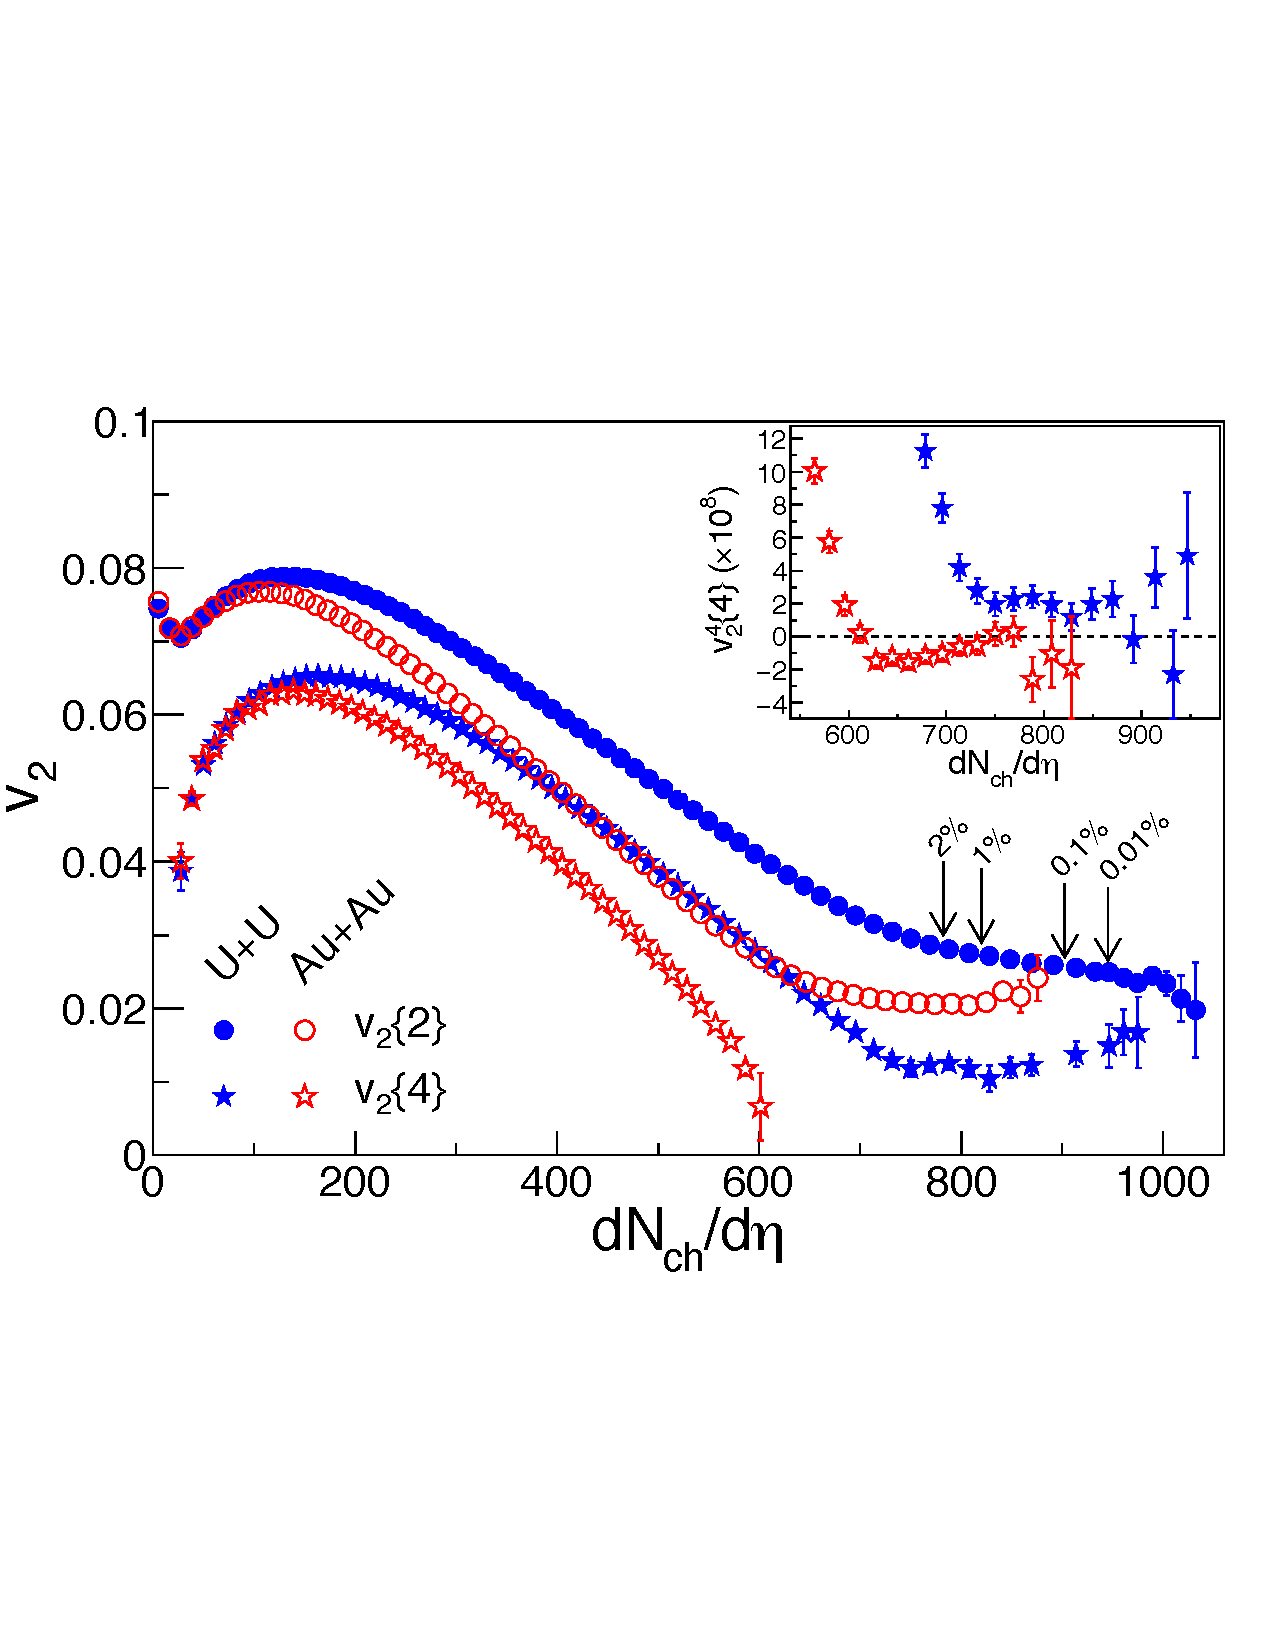
\includegraphics[width=.6\linewidth]{figs/chapter_centfluc/STAR_AuAu_centfluc.pdf}
\caption{The two- and four-particle cumulant $v_2\{2\}$ and $v_2\{4\}$ within $|\eta|<1$ versus $d\Nch/d\eta$ from 200 GeV Au+Au and 193 GeV U+U collisions. Dashed lines show U+U centralities based on $d\Nch/d\eta$ measured in $|\eta|<0.5$. $v_2^4\{4\}$ is shown in the inset without taking the fourth root in the range where it is near zero or negative. This figure is taken from Ref.~\cite{Adamczyk:2015obl}.}
\label{fig:centfluc_STAR_AuAu_centfluc}
\end{figure}

This sign change clearly indicates a non-Gaussian flow fluctuation in ultra-central Au+Au collisions, however, model studies all predict a Gaussian $p(\epsilon)$ from initial state. This could mean:
\begin{itemize}
\item $p(\epsilon)$ is not Gaussian, which challenges the initial state models;
\item Or $v_n$ is not linear to $\epsilon_n$, which challenges the hydrodynamic models;
\end{itemize}
But before we begin to worry and modify the models, there might be another simple mechanism: centrality fluctuation. In the later sections, we will see why centrality fluctuation can explain the sign change of $c_2\{4\}$ in ultra-central collisions.



\subsection{Centrality fluctuation}

Centrality is an important concept for heavy-ion collisions, which characterizes the amount of overlap or size of fireball in the collision region. Conceptually, the definition of centrality is not unique; people often use~\cite{Miller:2007ri, Loizides:2014vua, Adler:2013aqf}:
\begin{itemize}
\item the number of nucleons $N_\text{part}$ in the overlap region also known as participants or wounded nucleons;
\item the two-component model where the event activity is theorized to be proportional to a linear combination of $N_\text{part}$ and number of binary nucleon-nucleon collisions $N_\text{bin}$: $N_\text{an}\equiv (1-x)N_\text{part}/2 + x N_\text{bin}$, with $x$ being a tunable constant;
\item the number of constituent-quark participants $N_\text{qp}$ in the overlap region.
\end{itemize}
Since there quantities, generally referred to as the number of sources $N_\text{s}$, are not directly measurable, a Glauber model that includes nuclear geometry and particle production is often used to connect the $N_\text{s}$ with the experimentally measured event activity $\text{cent}_\text{obs}$, such as the number of charge particles $\Nch$ or the total transverse energy $\Et$ in a given rapidity range. The Glauber model also provides estimates for many other parameters that describe the initial collision geometry, such as eccentricities $\epsilon_n$, which describes the azimuthal asymmetry in the distribution of the sources in the transverse plane.



\subsubsection{Origin}

In data analysis, the centrality estimator is usually defined as the reference particle multiplicity $N_\text{A}$ in a forward pseudorapidity window A, $\text{cent}_\text{obs} \equiv N_\text{A}$, and the observables of interest are measured using particles in a different pseudorapidity window B, usually around middle rapidity. Because of fluctuations in particle production, events with the same $N_\text{s}$ may have different values of $\text{cent}_\text{obs}$. Conversely, events selected with the same $\text{cent}_\text{obs}$ can have different values of $N_\text{s}$. If a physics observable measured in the subevent B changes with $N_\text{s}$, its fluctuation would be affected by $N_\text{s}$ fluctuation associated with centrality selection defined on $N_\text{A}$.

The fluctuation of $N_\text{s}$ for fixed $\text{cent}_\text{obs}$ value is commonly referred to as ``volume fluctuation''~\cite{Jeon:2003gk, Skokov:2012ds, Luo:2013bmi}, which is an irreducible ``centrality fluctuation'' (CF). The CF is large in peripheral collisions or small collision systems where it often dominates the uncertainties in $N_\text{s}$ estimation. The CF is expected to be strongly distorted in Ultra-Central Collisions (UCC) due to the steeply falling distribution of $p(N_\text{s})$~\cite{Skokov:2012ds, Xu:2016qzd, Bzdak:2016jxo}.



\subsubsection{Influences on other measurements}

The CF also contributes to the measurements of event-by-event fluctuations of conserved quantities and is one of the main source of model uncertainty for extraction of the final-state dynamical fluctuations~\cite{Aggarwal:2010wy, Adamczyk:2013dal, Adamczyk:2014fia} associated with the critical endpoint in the QCD phase diagram~\cite{Luo:2017faz, Li:2017via}. There have been extensive studies of CF using multiplicity cumulants. Skokov $et\text{ }al.$~\cite{Skokov:2012ds} first pointed out the importance of CF for multiplicity fluctuation measurement and derived a general formula relating multiplicity cumulants to the CF within an independent source model framework. Most studies focused on the impact of CF on cumulants for conserved charge, e.g., net proton, for the search of critical endpoint in the RHIC beam energy scan program~\cite{Luo:2013bmi, Braun-Munzinger:2016yjz, Kitazawa:2017ljq}

Any observable that is sensitive to $p(N_\text{s})$ fluctuation can be used to study the CF through the multi-particle cumulants of this observable. Besides the multiplicity fluctuation $p(N)$, we also use the fluctuation of harmonic flow $v_n$ to probe the CF effects. The basic idea is the following: Hydrodynamical simulations show that $v_n$ are driven by the eccentricity $\epsilon_n$ of the initial collision geometry, $v_n \propto \epsilon_n$, for $n=2$ and 3~\cite{Qiu:2011iv, Gardim:2011xv, Niemi:2012aj}. Since the sources determining the event centrality also control $\epsilon_n$ of the event, the fluctuation of $N_\text{s}$ from CF gives rise to additional fluctuations in $\epsilon_n$, which in turn generates additional fluctuations in $v_n$. In order to test CF in data without model assumptions, two reference event class definitions are used to study the influence of centrality fluctuations on flow cumulants.



\subsection{Methodology}

\subsubsection{Glauber model}
\label{sec:glauber_model}

Figure~\ref{fig:centfluc_cartoon_particle_production} illustrates the particle production mechanism used in this model study. Particle production is simulated with a simple independent source model, where the total particle multiplicity in each A+A collision is calculated as a sum of particles from each source via a common probability distribution. The sources could be participating nucleons, those given by two component model, or participating constituent quarks and they are generated using a Glauber model framework~\cite{Miller:2007ri}. Quantities describing the collision geometry, such as the transverse area or the eccentricities $\epsilon_n$, can be obtained from transverse positions $(x, y)$ of the sources. The present study does not model explicitly the sub-nucleonic degree of freedom, and the number of of sources $N_\text{s}$ therefore represents either the $N_\text{part}$ (the wounded nucleon or WN model) or $N_\text{an}\equiv (1-x) N_\text{part}/2 + x N_\text{bin}$ (the two-component model). However, it is pointed out~\cite{Adler:2013aqf} that the $N_\text{an}$ and associated nuclear geometry is a good proxy for the number of participating constituent quarks and their associated nuclear geometry.

\begin{figure}[H]
\centering
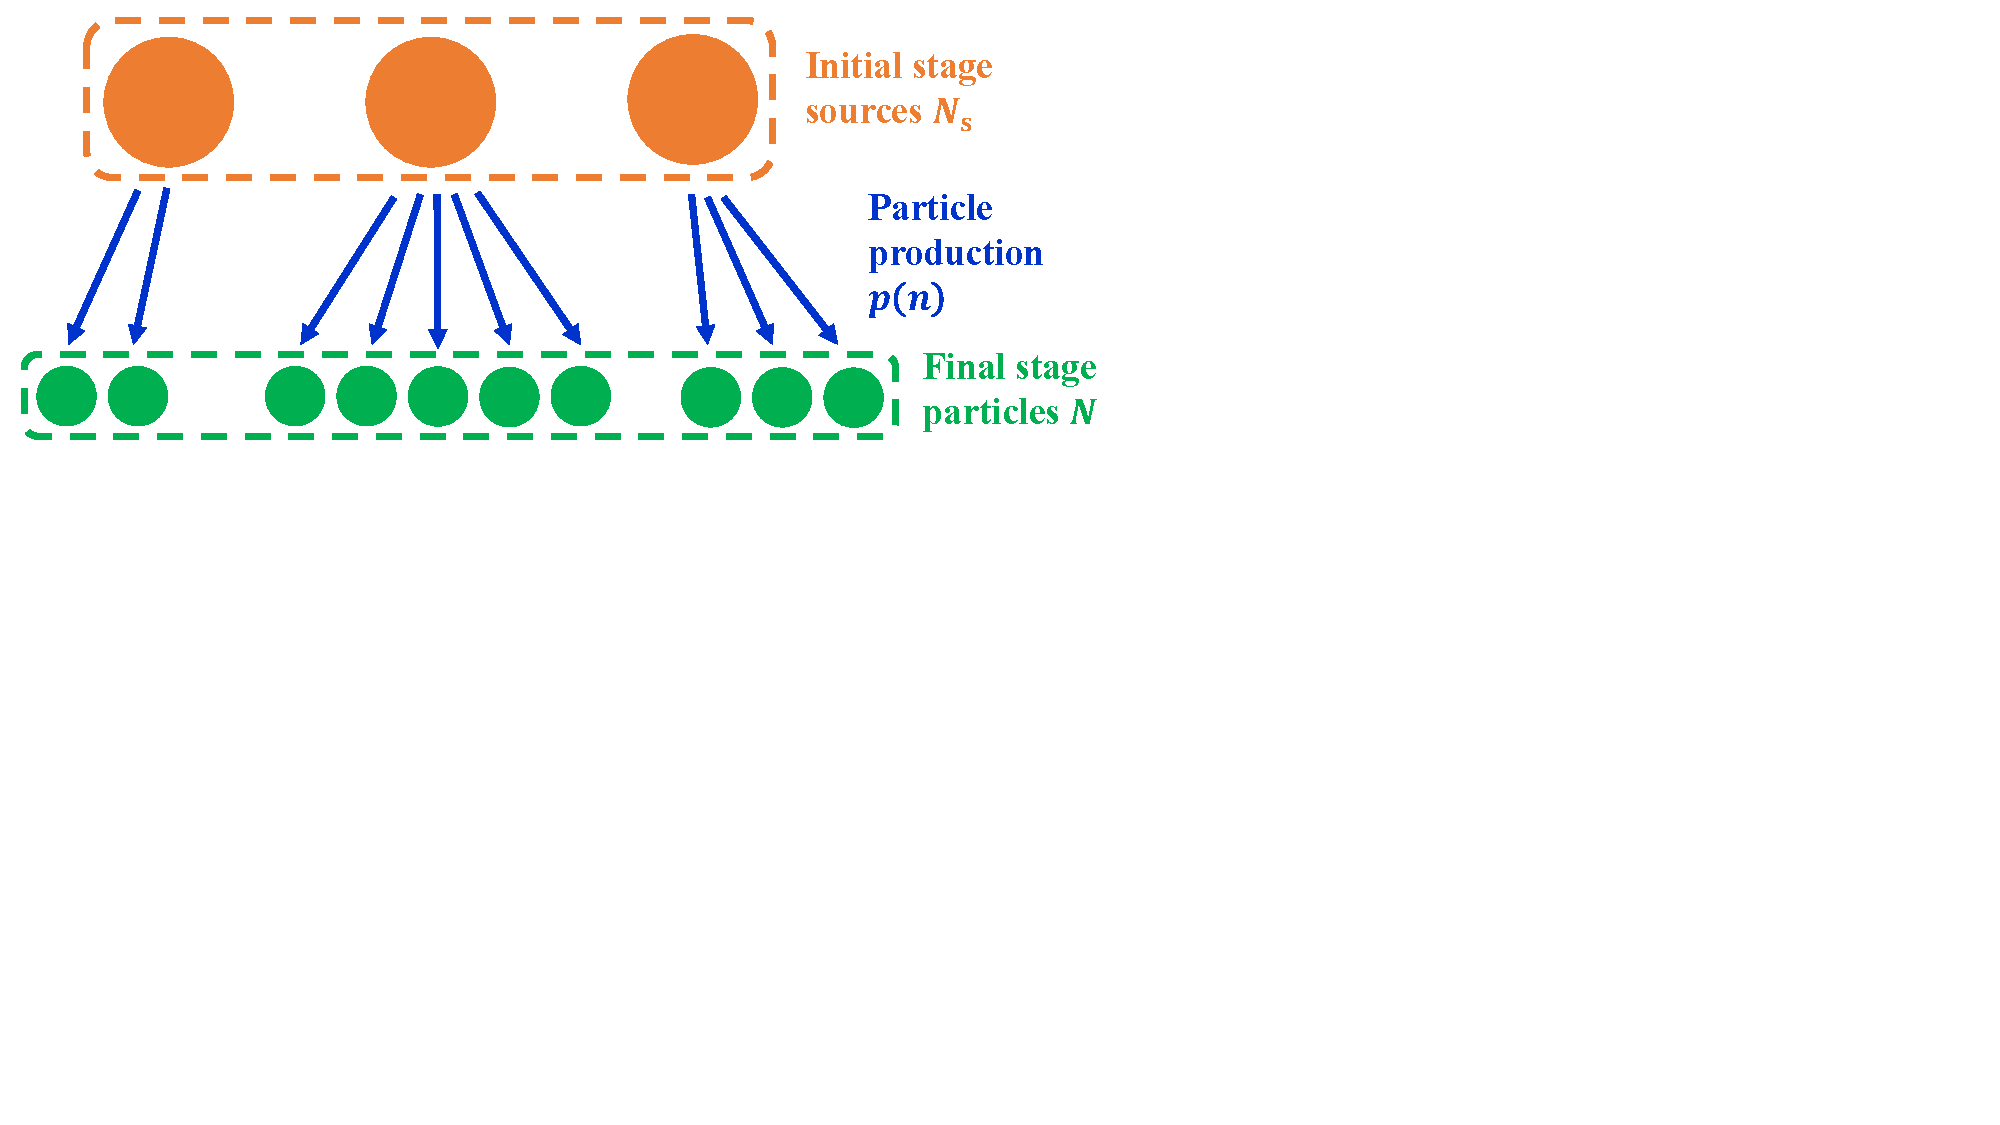
\includegraphics[width=.75\linewidth]{figs/chapter_centfluc/cartoon_particle_production.pdf}
\caption{Cartoon showing particle production mechanism. From top to bottom: independent source, particle production in each source and observed total number of particles.}
\label{fig:centfluc_cartoon_particle_production}
\end{figure}

The particle production from each source is assumed to follow a Negative Binomial Distribution (NBD):
\begin{equation}
p_\text{NBD}(n;m,p) = \frac{(n+m-1)!}{(m-1)!n!} p^n (1-p)^m, p=\frac{\bar{n}}{\bar{n}+m},
\end{equation}
where $\bar{n}$ is the average number of particle in the acceptance and $p$ is the probability of a particle falling into the acceptance. This form has been widely used to describe the multiplicity distributions in $pp$ collisions~\cite{Ghosh:2012xh}. One important property of the NBD for our study is its relative width $\sigma$:
\begin{equation}
\sigma^2 \equiv \frac{\lr{(n-\bar{n})^2}}{\bar{n}^2} = \frac{1}{\bar{n}} + \frac{1}{m},
\end{equation}
which controls the strength of the fluctuation for each source. 

The distribution of total multiplicity is obtained as a superposition of the NBD distributions from all sources:
\begin{equation}
\begin{split}
N &= n_1 + n_2 + \cdot\cdot\cdot + n_{N_\text{s}} \\
p(N) &= p_\text{NBD}(n_1;m,p) \otimes p_\text{NBD}(n_2;m,p) \otimes \cdot\cdot\cdot \otimes p_\text{NBD}(n_{N_\text{s}};m,p) \\
&= p_\text{NBD}(N; mN_\text{s}, p)
\end{split}
\end{equation}
where we used the additive nature of the NBD distributions for convolution. One interesting consequence of this feature is that we can subdivide the multiplicity distribution into sources with smaller number of particles:
\begin{equation}
p_\text{NBD}(N; mN_\text{s}, p) = p_\text{NBD}(n_1; m/k, p) \otimes p_\text{NBD}(n_2; m/k, p) \otimes \cdot\cdot\cdot \otimes p_\text{NBD}(n_{N_\text{s}}; m/k, p),
\end{equation}
where each source is subdivided into $k$ identical sources with smaller average $\bar{n}/k$ but the same $p$, without changing the total multiplicity distribution. In this case, Glauber models with and without explicit treatment of sub-nucleonic degree of freedom would be identical to each other, unless $k$ is allowed to fluctuate for each wounded nucleon.

The distribution of sources in the collision zone is described by a standard Glauber model for various collision systems. The nucleons are assumed to have a hard core of 0.3 fm in radii; their transverse positions are generated according to the Woods-Saxon distribution~\cite{Loizides:2014vua}. A nucleon-nucleon cross section of $\sigma = 68$ mb is used to simulate the collisions at $\sqrt{s_\text{NN}}=5.02$ TeV. The usual geometric quantities, including $N_\text{part}$, $N_\text{bin}$ and $\epsilon_n$, are calculated for each event. The $N_\text{an}$ in the two-component model is given by choose $x=0.09$, very close to those used at the top RHIC energy~\cite{Adler:2013aqf}, which was shown to approximately describe the multiplicity distribution in A+A collisions~\cite{Adler:2013aqf, Abelev:2013qoq}.

Table~\ref{table:centfluc_Glauber_pars} lists the NBD parameters for the wounded nucleon model and two-component model. The three parameter sets, Par0, Par1 and Par2, have the same $\bar{n}$ but different $\hat{\sigma}$. The Par0 and Par1 sets are adjusted to approximately describe the shapes of the experimental $\Nchrec$ ($|\eta|<2.5$) and $\Et$ ($3.2<|\eta|<4.9$) distributions from the ATLAS Collaboration~\cite{ATLAS-CONF-2017-066}, while the Par2 set corresponds to a case with much larger fluctuation.

\begin{table}[H]
\centering
\begin{tabular}{|lcccc|}
\hline
\multicolumn{5}{|c|}{Wounded nucleon model}                                                                                                                                \\ \hline
                           & \multicolumn{1}{l}{$p$}    & \multicolumn{1}{l}{$m$}    & \multicolumn{1}{l}{mean $\bar{n}$} & \multicolumn{1}{l|}{rms / mean $\hat{\sigma}$} \\ \hline
\multicolumn{1}{|l|}{Par0} & \multicolumn{1}{c|}{0.688} & \multicolumn{1}{c|}{3.45}  & \multicolumn{1}{c|}{7.6}           & 0.65                                           \\ \hline
\multicolumn{1}{|l|}{Par1} & \multicolumn{1}{c|}{0.831} & \multicolumn{1}{c|}{1.55}  & \multicolumn{1}{c|}{7.6}           & 0.88                                           \\ \hline
\multicolumn{1}{|l|}{Par2} & \multicolumn{1}{c|}{0.928} & \multicolumn{1}{c|}{0.593} & \multicolumn{1}{c|}{7.6}           & 1.35                                           \\ \hline
\multicolumn{5}{|c|}{Two-component model}                                                                                                                                  \\ \hline
                           & \multicolumn{1}{l}{$p$}    & \multicolumn{1}{l}{$m$}    & \multicolumn{1}{l}{mean $\bar{n}$} & \multicolumn{1}{l|}{rms / mean $\hat{\sigma}$} \\ \hline
\multicolumn{1}{|l|}{Par0} & \multicolumn{1}{c|}{0.391} & \multicolumn{1}{c|}{13.7}  & \multicolumn{1}{c|}{8.7}           & 0.43                                           \\ \hline
\multicolumn{1}{|l|}{Par1} & \multicolumn{1}{c|}{0.738} & \multicolumn{1}{c|}{3.10}  & \multicolumn{1}{c|}{8.7}           & 0.66                                           \\ \hline
\multicolumn{1}{|l|}{Par2} & \multicolumn{1}{c|}{0.909} & \multicolumn{1}{c|}{0.878} & \multicolumn{1}{c|}{8.7}           & 1.12                                           \\ \hline
\end{tabular}
\caption{The various parameter sets for the NBD used for modeling the particle production in the wounded nucleon model (top) and two-component model (right).}
\label{table:centfluc_Glauber_pars}
\end{table}

The distributions generated from the three parameter sets are rescaled horizontally by the knee, defined as the average multiplicity for $2A=416$ nucleons for Pb+Pb collisions, $N_\text{knee}=2A\bar{n}$. Figure~\ref{fig:centfluc_Glauber_Ndis} shows the three rescaled distributions for the wounded nucleon model (left) and two-component model (right), respectively. They are compared to the $\Nchrec$ or $\Et$ distributions, which are also rescaled by the knee values obtained for Par0 and Par1, respectively. The two-component model slightly better describes the shape of the data, because the source distribution from the two-component model $p(N_\text{an})$ has a smoother and broader knee than that given by the wounded nucleon model $p(N_\text{part})$. The relative widths $\hat{\sigma}$ for each source, therefore, are also much smaller for the two-component model than the wounded nucleon model. One important consequence is that once the generated $p(N)$ distribution is tuned to have similar shape (i.e., by matching to the same experimental measured $p(\Nchrec)$ distribution), the centrality fluctuations are typically larger in the wounded nucleon model than the two-component model as the same total multiplicity, which will be shown in Section~\ref{sec:glauber_model}.

\begin{figure}[H]
\centering
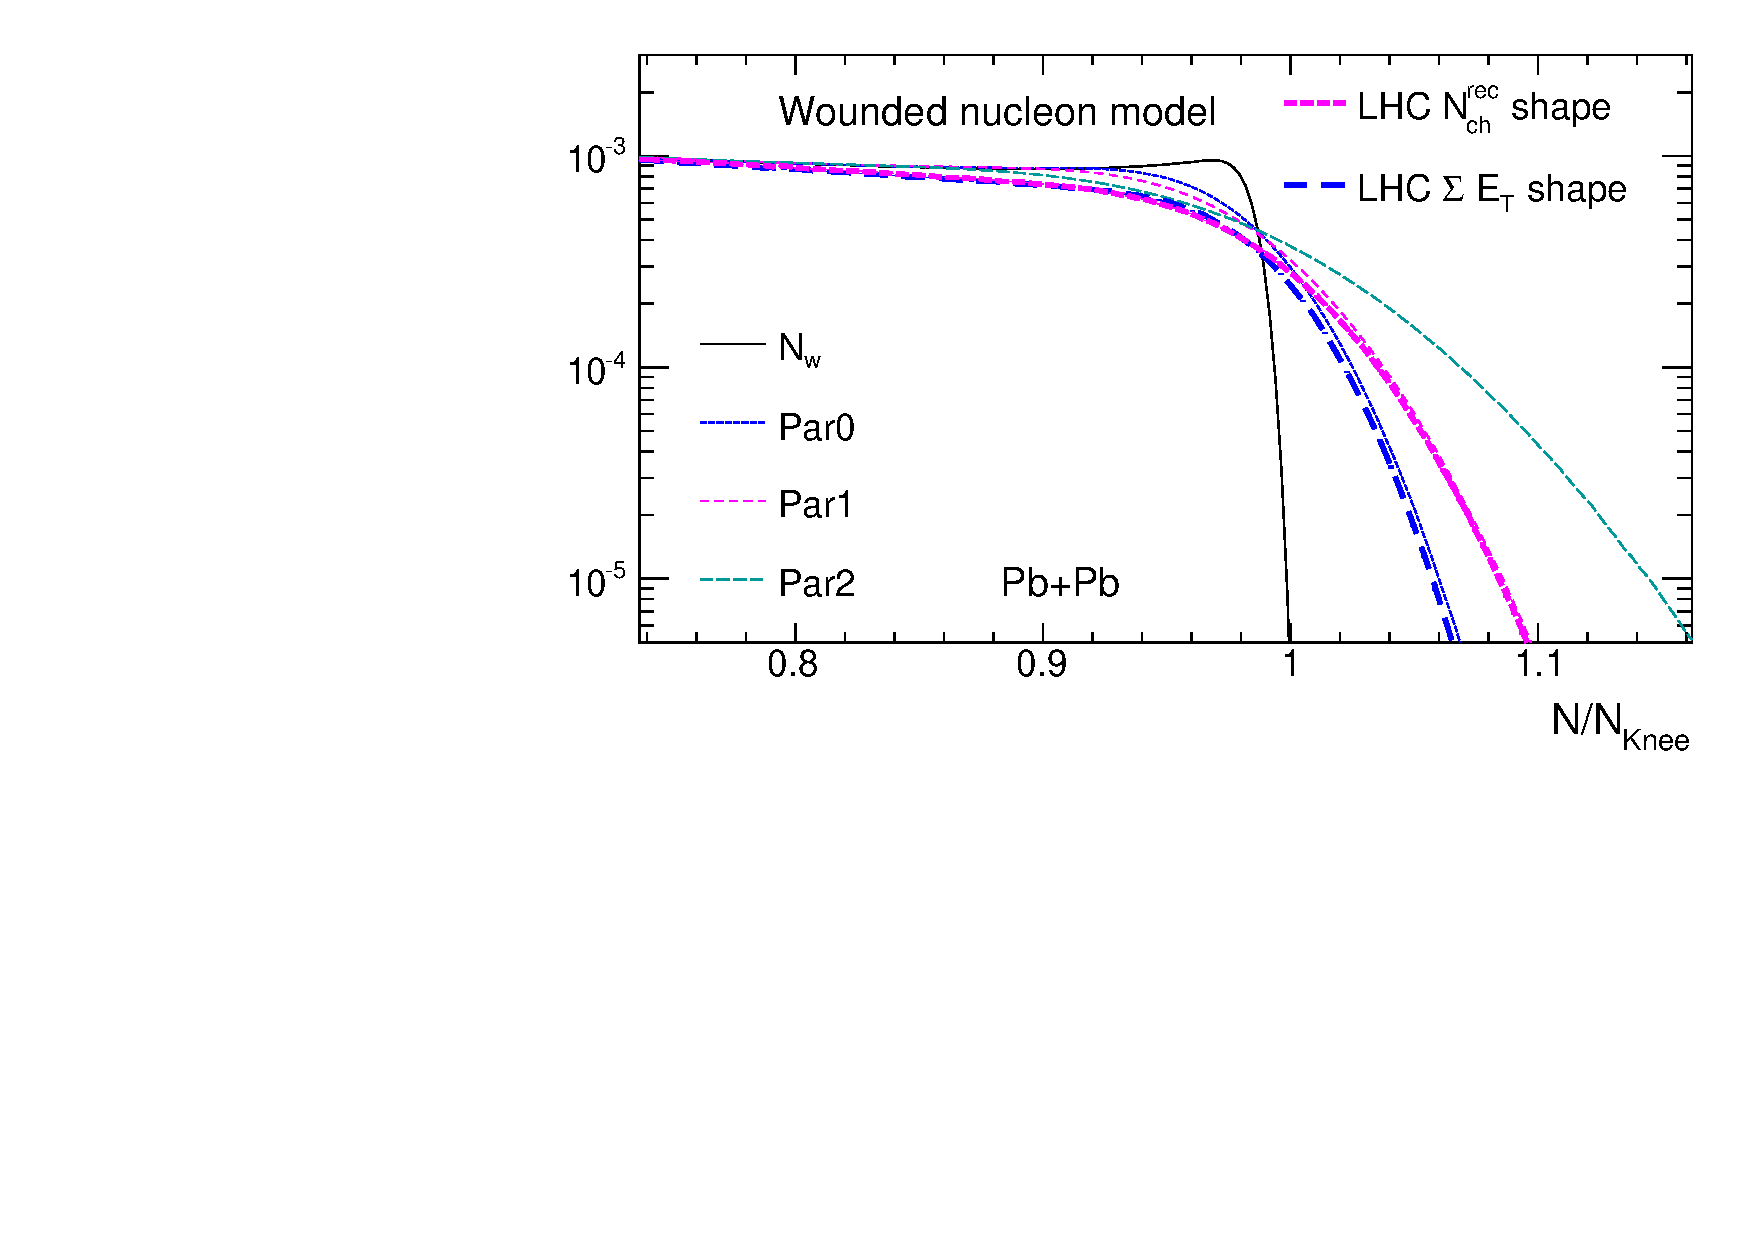
\includegraphics[width=.475\linewidth]{figs/chapter_centfluc/Glauber_Ndis_Nw.pdf}
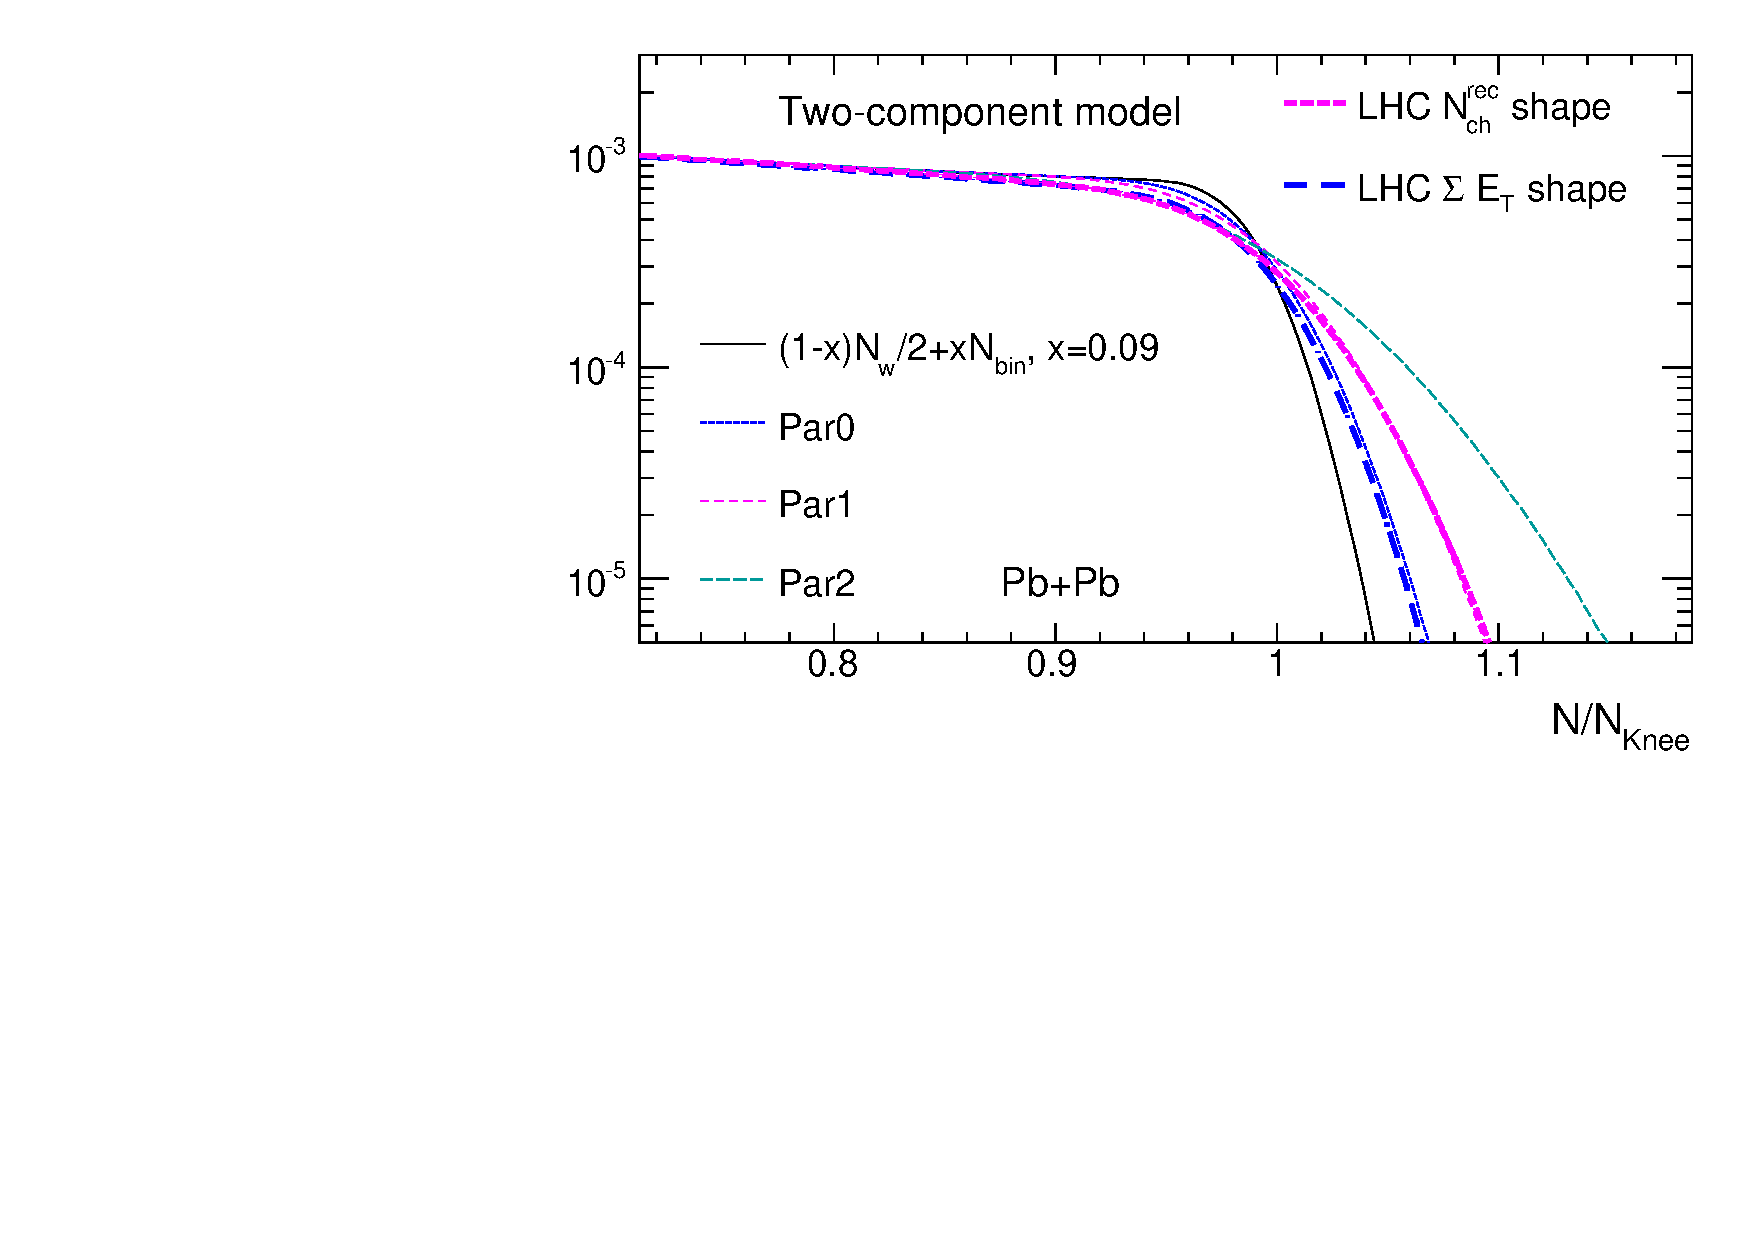
\includegraphics[width=.475\linewidth]{figs/chapter_centfluc/Glauber_Ndis_Nan.pdf}
\caption{The distributions of sources and produced particles based on two parameter sets, rescaled by their knee values as described in the text for the wounded nucleon model (left) and two-component model (right). They are compared with the shapes of the experimental $\Nchrec$ ($|\eta|<2.5$) and $\Et$ ($3.2<|\eta|<4.9$) distributions.}
\label{fig:centfluc_Glauber_Ndis}
\end{figure}

Obviously, the independent source model based on Glauber and NBD has certain limitations on its predictive power. It does not model the interaction between different sources, which clearly is important in the final state. These interactions may modify the particle correlations in each source or create new sources of fluctuations. Our model also assumes explicitly that $N_\text{s}$ is the same independent of rapidity. In reality, the $N_\text{s}$ and the length of the source in rapidity are expected to have strong fluctuations~\cite{Bozek:2015bna, Pang:2015zrq, Schenke:2016ksl}. For example, the sub-nucleonic degree of freedom may evolve with rapidity, such that the number of sources for each nucleon is not the same between middle rapidity and forward rapidity~\cite{Schenke:2016ksl, Jia:2015jga}. These longitudinal fluctuations tend to weaken the centrality correlation between the forward and middle rapidity, such that the CF in forward rapidity may not be the same as that at middle rapidity. Nevertheless, our model studies serve as a useful baseline. It can be considered as a first step toward a more realistic simulation that includes the full space-time dynamics of the heavy-ion collisions.



\subsubsection{ATLAS data}

In data analysis, since initial stage quantities $N_\text{part}$ and $N_\text{an}$ are unknown, out of the six parameter sets shown in Table~\ref{table:centfluc_Glauber_pars}, only Par0 ($\Et$) and Par1 ($\Et$) are included in this study. The left panel of Figure~\ref{fig:centfluc_ATLAS_corr_Et_Nch} shows the correlation between $\Et$ and $\Nchrec$. The two quantities have an approximately linear correlation, but events with the same $\Et$ have significant fluctuations in $\Nchrec$ and vice versa. Due to this relative fluctuations, reference event class based on $\Nchrec$ may have different centrality fluctuations from reference event class based on $\Et$, even if both are matched to have the same $\lr{\Et}$ or the same $\lr{\Nchrec}$.

\begin{figure}[H]
\centering
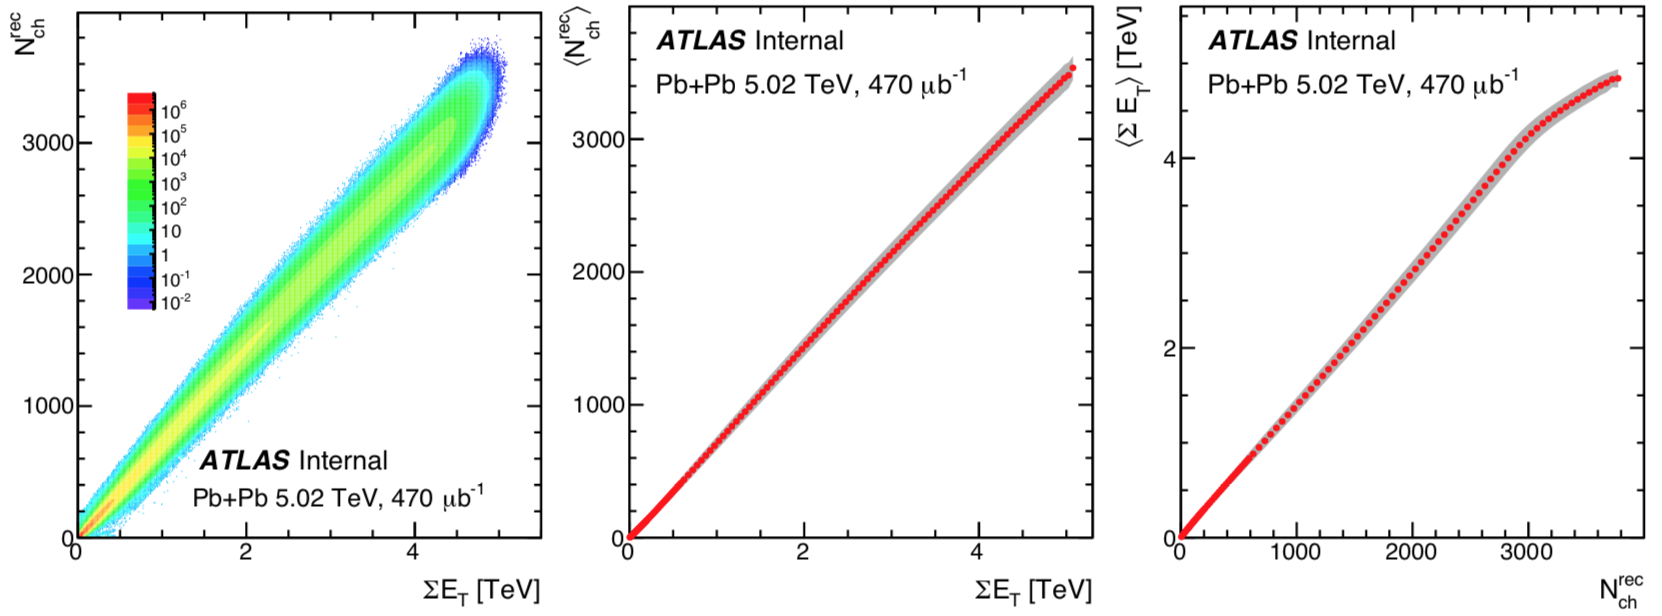
\includegraphics[width=.95\linewidth]{figs/chapter_centfluc/ATLAS_corr_Et_Nch.png}
\caption{The correlation between $\Nchrec$ and $\Et$ (left), and the mean (solid points) and root-mean-square (shaded bands) of either the $\Nchrec$ distributions for events in narrow slices of $\Et$ (middle) or the $\Et$ distributions for events in narrow slices of $\Nchrec$ (right).}
\label{fig:centfluc_ATLAS_corr_Et_Nch}
\end{figure}

To quantify the correlation between $\Et$ and $\Nchrec$, events are divided into narrow intervals in $\Et$ $(\Nchrec)$, and the mean and root-mean-square values of the $\Et$ $(\Nchrec)$ distributions are calculated for each interval. The results are shown in the middle and right panels of Figure~\ref{fig:centfluc_ATLAS_corr_Et_Nch}, respectively. A linear relation is observed between $\lr{\Nchrec}$ and $\Et$ over the full $\Et$ range, while a significant non-linear relation is observed between $\lr{\Et}$ and $\Nchrec$ at large $\Nchrec$. This latter behavior suggests that, in ultra-central collisions, $\Et$ retains sensitivity to the $\lr{\Nchrec}$ of the events ,while $\Nchrec$ has relatively poorer sensitivity to the $\lr{\Et}$ of the events. This suggests that the true centrality is more smeared for events with the same $\Nchrec$ than events with the same $\Et$.

Since $v_n$ changes with centrality, any centrality fluctuations could lead to additional fluctuation of $v_n$, and subsequently a change in the flow cumulants. Indeed, subevent cumulant results in Section~\ref{chapter:subcumu} has shown that the $c_n\{2k\}$ values depend on the definition of reference event class used for averaging. A comparison of the results based on these two reference event classes, can shed light on the details of flow fluctuations and how they are affected by centrality fluctuation.

To illustrate how the rescaling is performed, Figure~\ref{fig:centfluc_ATLAS_dis_Et_Nch} shows the distributions of $\Nchrec$ and $\Et$ obtained from the two-dimensional correlation in the left panel of Figure~\ref{fig:centfluc_ATLAS_corr_Et_Nch}. The inserted panels show the local first-order derivatives of the one-dimensional $\Et$ or $\Nchrec$ distributions in the most central collisions. The derivative for the $\Et$ distribution is relatively independent of $\Et$ up to 4.1 TeV and then decreases and reaches a local minimum at around 4.4 TeV; the derivative for the $\Nchrec$ distribution is mostly flat up to 2800 and then decreases and reaches a local minimum at around 3100. The location where the derivative starts to depart from a constant is defined as the knees of the $\Et$ or $\Nchrec$ distributions: $(\Et)_\text{knee} = 4.1$ TeV and $(\Nchrec)_\text{knee} = 2800$. These knees mark the locations where multiplicity distributions start to decrease sharply, and the underlying centrality fluctuations are expected to deviate significantly from a Gaussian distribution~\cite{Zhou:2018fxx, Xu:2016qzd}.

\begin{figure}[H]
\centering
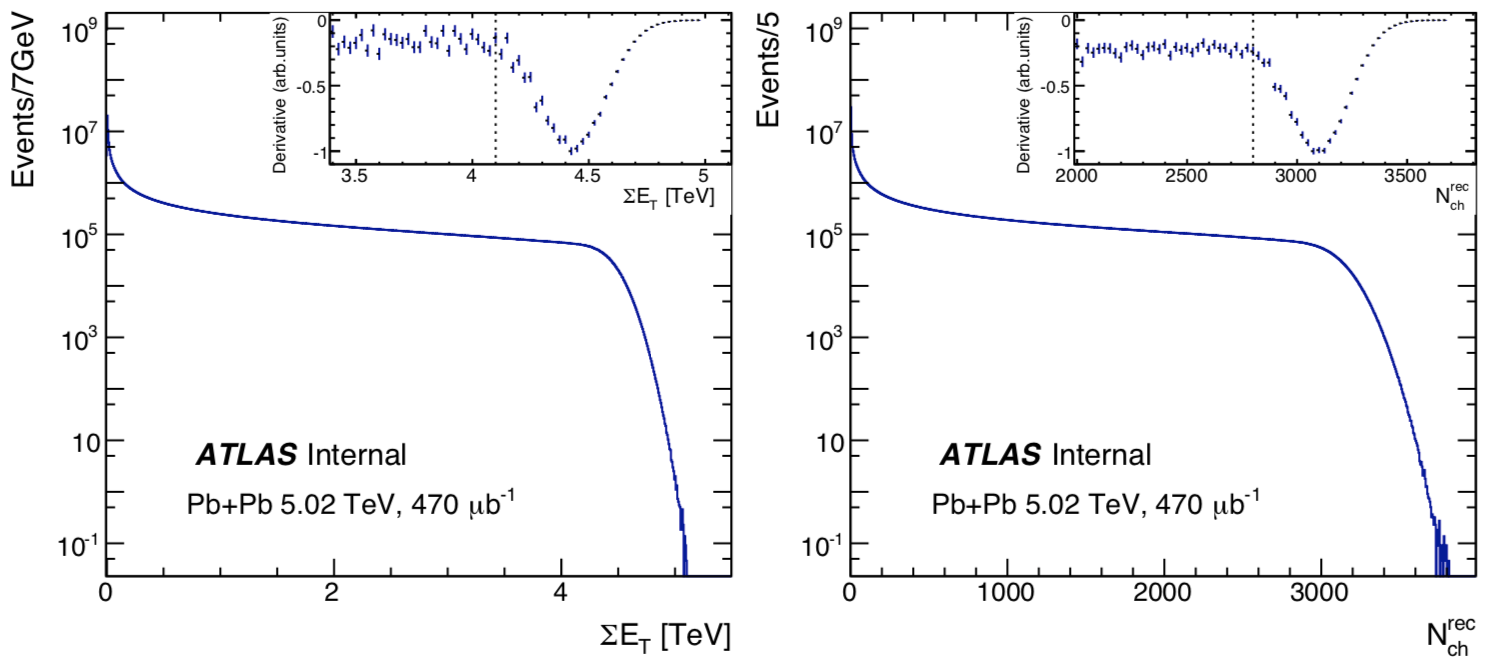
\includegraphics[width=.95\linewidth]{figs/chapter_centfluc/ATLAS_dis_Et_Nch.png}
\caption{The distribution of $\Et$ (left) and the distribution of $\Nchrec$ (right) for the Pb+Pb collisions. The inserted panels show the first-order derivative of the corresponding one-dimensional distributions, and the vertical dashed line indicate the location where the derivatives start to decrease, $(\Et)_\text{knee}=4.1$ TeV and $(\Nchrec)_\text{knee}=2800$, respectively. The values of the derivatives have been rescaled to a minimum value of -1.}
\label{fig:centfluc_ATLAS_dis_Et_Nch}
\end{figure}



\subsubsection{Observable}

In this section, we will list all the observables measured to test the CF. Notation $v_n$ is used for the flow cumulant, while in the Glauber model, all the formulas are the same: simply replace $v_n$ with $\epsilon_n$:
\begin{equation}
\epsilon_n = -\frac{\lr{r^n e^{\text{i}m\phi}}}{\lr{r^n}}
\end{equation}
where $(r, \phi)$ are the transverse positions of the particle production sources. Most of the flow cumulant formulas, with both standard and subevent methods, have been introduced in Section~\ref{chapter:subcumu}. In this section, normalized cumulants and cumulant ratios are added.

Any quantity which is linearly proportional to $v_n$ has the same cumulants, up to a global factor. Therefore the shapes of $p(v_n)$ and $p(v_n, v_m)$ can be more directly probed using the ratio of the cumulants~\cite{Giacalone:2016afq, Das:2017ned}:
\begin{equation}
\begin{split}
nc_n\{4\} &= \frac{c_n\{4\}}{c_n^{b|c}\{2\}^2} \\
nc_n\{6\} &= \frac{c_n\{6\}}{4 c_n^{b|c}\{2\}^3} \\
nsc_{n,m}\{4\} &= \frac{sc_{n,m}\{4\}}{c_n^{b|c}\{2\} c_m^{b|c}\{2\}} \\
nac_n\{3\} &= \frac{ac_n\{3\}}{\sqrt{(2c_n^{b|c}\{2\}^2 + c_n\{4\}) c_{2n}^{b|c}\{2\}}}
\end{split}
\end{equation}
where two-particle cumulants $c_n\{2\}$ in the denominator of these equations are calculated from subevent $b$ and $c$. If $v_n$ is exactly proportional to $\epsilon_n$, the normalized cumulants defined above would be the same as the normalized cumulants calculated from eccentricities in the initial state. In practice, final state effects, such as $\pT$-dependent fluctuation of $v_n$ and $\Phi_n$~\cite{Gardim:2012im, Heinz:2013bua}, hydrodynamic noise~\cite{Akamatsu:2016llw}, nonlinear mode-mixing between harmonics of different order~\cite{Gardim:2011xv, Teaney:2012ke} can break this equality. Therefore, studying the $\pT$ dependence of these normalized cumulants can help to understand the influence of dynamical effects from the final state.



\subsection{Results}

In this section we show the results both for Glauber model and ATLAS data. For the Glauber model, we focus on the influences from the centrality fluctuation. For the ATLAS data, we first present the results of flow fluctuation, then discuss the impact of centrality fluctuation in a model-independent way.

\subsubsection{Glauber model}
\label{sec:glauber_model}

The top row of Figure~\ref{fig:centfluc_Glauber_nc2} shows the normalized cumulants $nc_2\{4\}$, $nc_2\{6\}$ and $nc_2\{8\}$ as a function of $\lr{N_\text{part}}$ in the wounded nucleon model. When eccentricity cumulants are calculated for events binned directly on $N_\text{part}$, the magnitudes of normalized cumulants decrease toward more central collisions, but they never change sign, i.e., $nc_2\{4\}<0$, $nc_2\{6\}>0$ and $nc_2\{8\}<0$ over the entire centrality range. However, when events are binned on generated particle multiplicity distribution $p(N)$, which is broader than $p(N_\text{part})$ due to particle production, a characteristic sign change is observed in central collisions. In particular, $nc_2\{4\}$ becomes positive , reaches a maximum, and then decreases to zero toward more central collisions. This finding is qualitatively similar to the sign-change behavior of $nc_2\{4\}$ observed in the ATLAS data~\cite{ATLAS-CONF-2017-066}, which we will show in Section~\ref{sec:cent_atlas_data}. Furthermore, as the relative width $\hat{\sigma}$ increases from that for Par0 to that for Par2, the location where $nc_2\{4\}$ crosses zero is shifted toward less central collisions and the maximum $nc_2\{4\}$ value increases. Our study also predicts more complex patterns of sign change for higher order cumulants when events are binned on generated particle multiplicity $p(N)$. For sufficient large $\hat{\sigma}$, the $nc_2\{6\}$ shows double sign change, and $nc_2\{8\}$ shows triple sign change in the central collision region.

The bottom row of Figure~\ref{fig:centfluc_Glauber_nc2} shows similar results calculated for the two-component model. It is interesting to see that the cumulants calculated for events binned directly on $N_\text{an}$ already exhibit sign changes in central collisions. This implies that the sign change is also sensitive to the nature of the fluctuations of the sources that drive the collective flow, not only on the smearing of sources by $p(n)$. After including particle production, the behavior of $nc_2\{2k\}$ shows qualitatively similar trends as those observed for the wounded nucleon model, but the magnitudes of $nc_2\{2k\}$ in the sign-change region are smaller.

\begin{figure}[H]
\centering
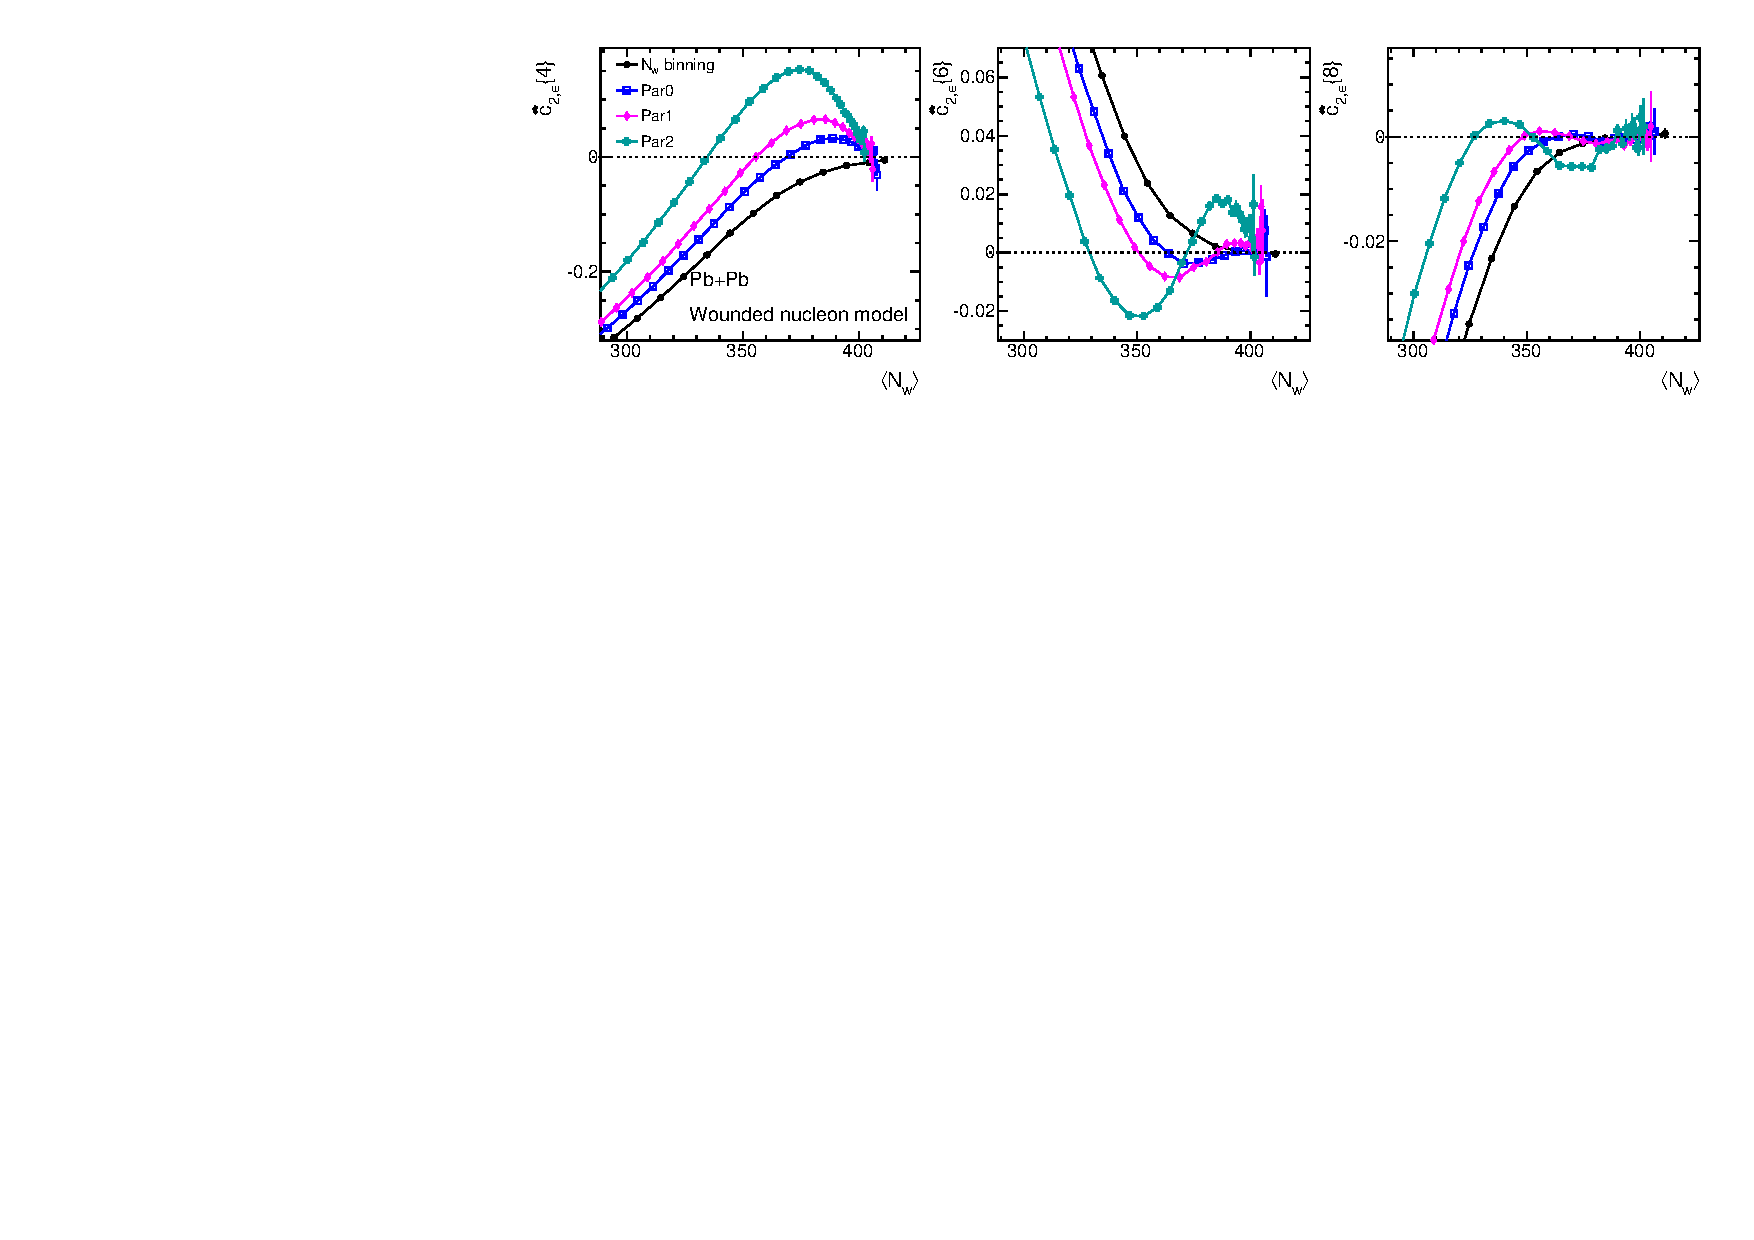
\includegraphics[width=.95\linewidth]{figs/chapter_centfluc/Glauber_nc2_Nw.pdf}
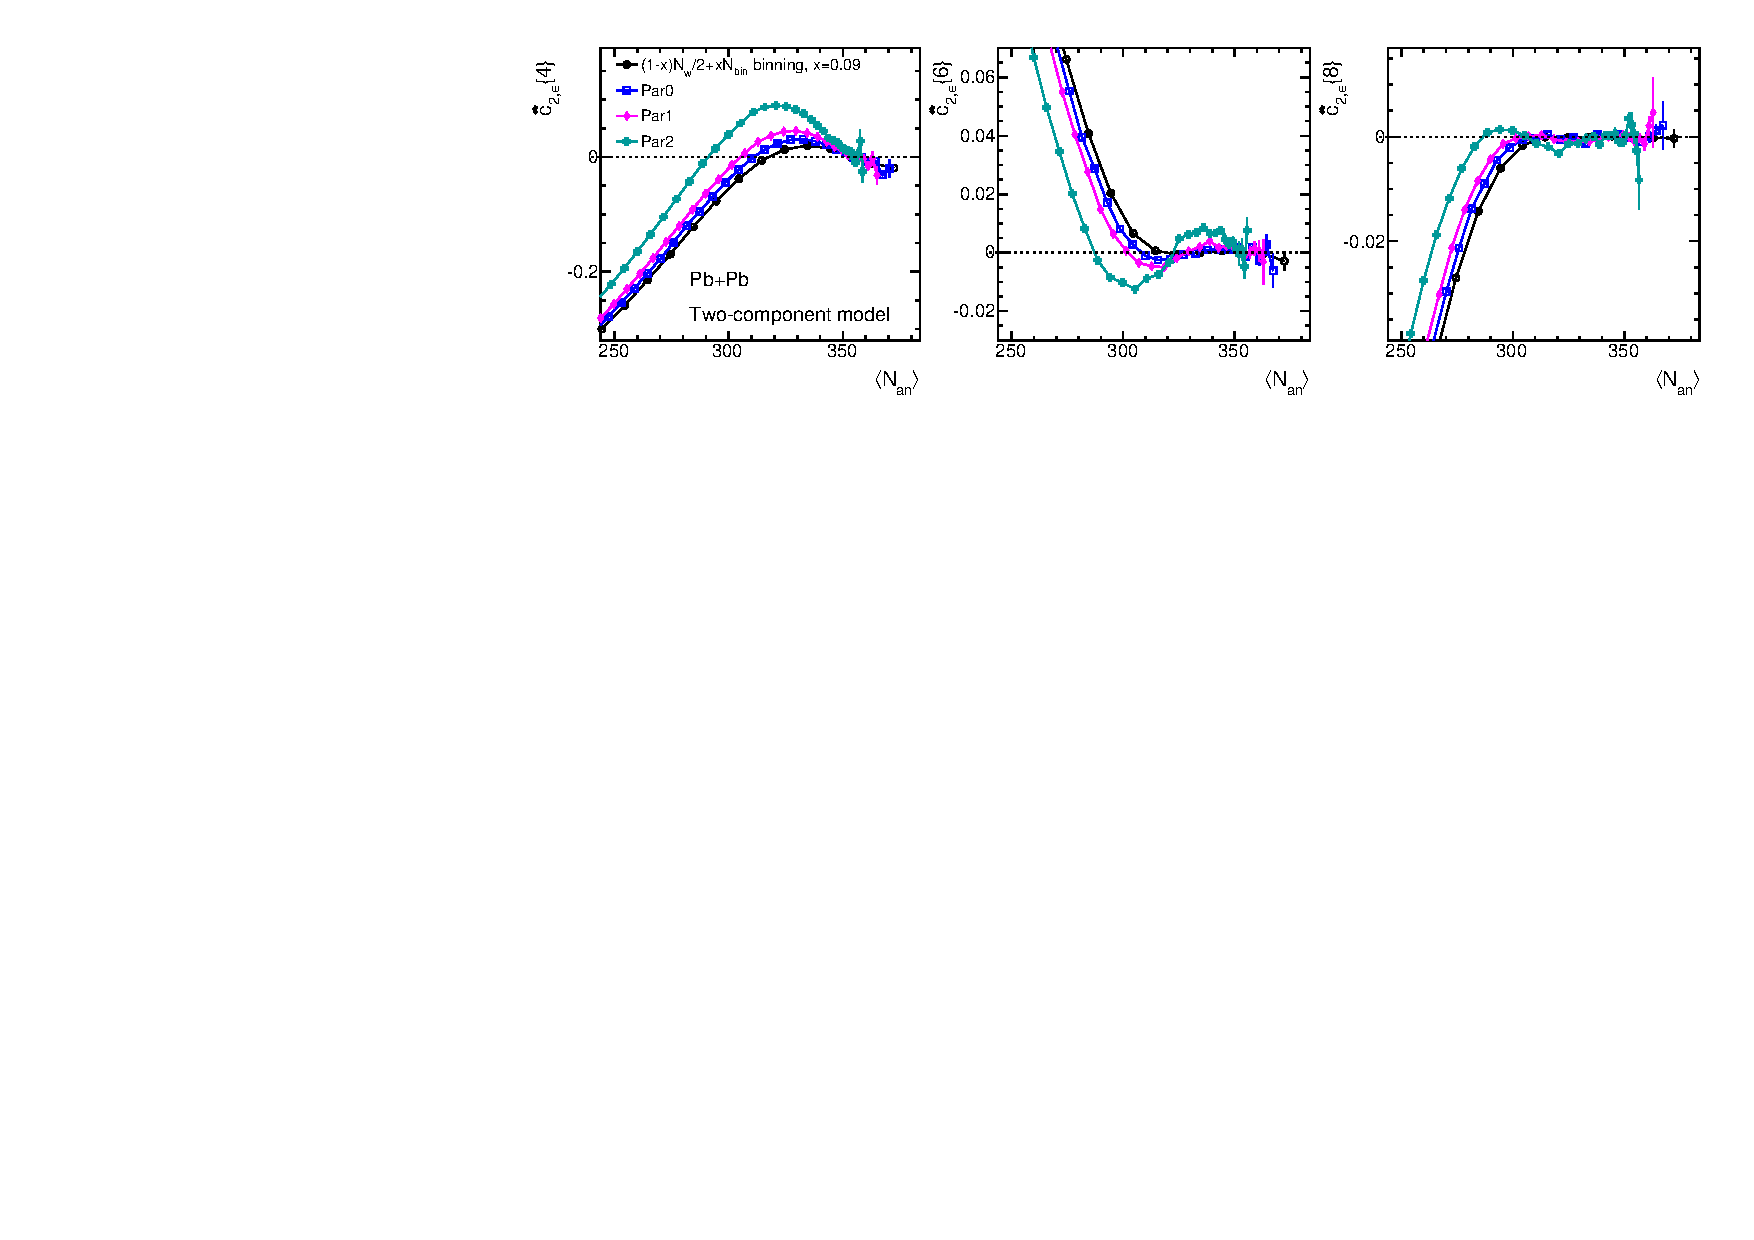
\includegraphics[width=.95\linewidth]{figs/chapter_centfluc/Glauber_nc2_Nan.pdf}
\caption{The normalized cumulants $nc_2\{4\}$ (left), $nc_2\{6\}$ (middle) and $nc_2\{8\}$ (right) for the three parameter sets for the wounded nucleon model (top row) and two-component model (bottom row). They are calculated in narrow particle multiplicity bins then combined and mapped to average number of sources.}
\label{fig:centfluc_Glauber_nc2}
\end{figure}

To further understand the origin of the sign-change behavior, we focus on $nc_2\{4\}$ shown in the top-left panel of Figure~\ref{fig:centfluc_Glauber_nc2}. We choose a particular range of multiplicity distribution $p(N)$ for the three parameter sets, corresponding to roughly the same $\lr{N_\text{part}}$. We then calculate the corresponding distributions of $N_\text{part}$ and scaled eccentricity $\epsilon_2 / \lr{\epsilon_2}$ for the selected events. We repeat this procedure in three different ranges and plot the corresponding distributions $p(N_\text{part})$ and $p(\epsilon_2 / \lr{\epsilon_2})$ in the three columns of Figure~\ref{fig:centfluc_Glauber_ecc}. The distributions $p(N_\text{part})$ and $p(\epsilon_2 / \lr{\epsilon_2})$ are different between the three parameter sets, even though they correspond to similar $\lr{N_\text{part}}$. This observation suggests that the sign change of $nc_2\{2k\}$ reflects the non-Gaussianity of $p(\epsilon_2 / \lr{\epsilon_2})$, which arises due to combining events with different $N_\text{part}$ and therefore different $p(\epsilon_2)$ shape.

\begin{figure}[H]
\centering
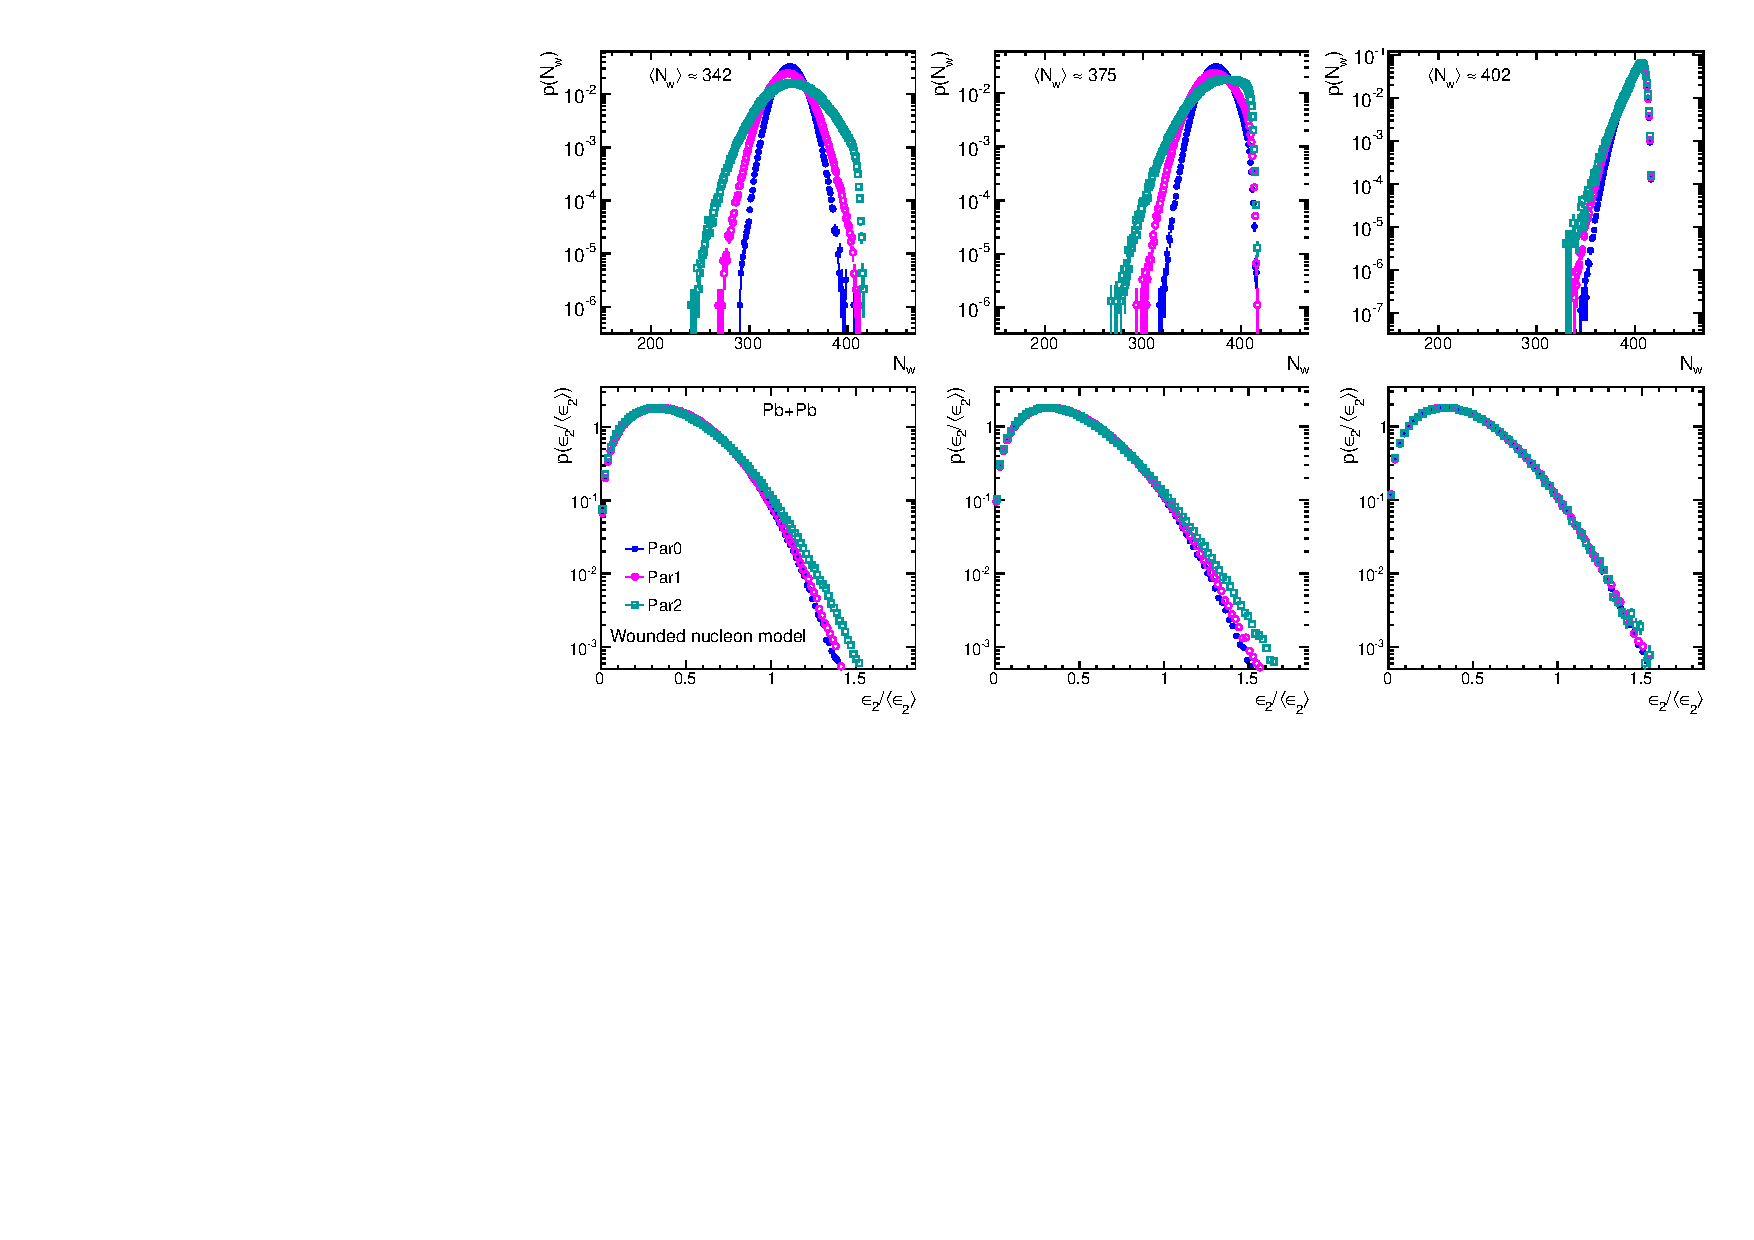
\includegraphics[width=.95\linewidth]{figs/chapter_centfluc/Glauber_ecc.pdf}
\caption{Distribution of $N_\text{part}$ (top row) and corresponding scaled eccentricity $\epsilon_2/\lr{\epsilon_2}$ (bottom row) for events selected in three range of particle multiplicity $N$ in the central collision region. The three curves in each panel corresponds to the three parameters sets for the wounded nucleon model.}
\label{fig:centfluc_Glauber_ecc}
\end{figure}

Top row of Figure~\ref{fig:centfluc_Glauber_others} shows the centrality dependence of other normalized cumulant observables, $nc_3\{4\}$, $nsc_{2,3}\{4\}$, $nsc_{2,4}\{4\}$ and $nac_{2}\{3\}$, calculated in the wounded nucleon model. The characteristic sign-change patterns are observed in central collisions except for $nac_2\{3\}$. As will be shown in Section~\ref{sec:cent_atlas_data}, ATLAS measurement also suggest similar sign-change patterns. We emphasize that it would be very interesting to measure $nsc_{2,3}\{4\}$, which should have better statistical precision that $nc_3\{4\}$. This observable is relatively insensitive to the final-state effects~\cite{Bilandzic:2013kga, Huo:2013qma, Aaboud:2017tql}, and therefore can be used to probe the initial centrality fluctuations. We have also repeated such studies for the two-component model (bottom row of Figure~\ref{fig:centfluc_Glauber_others}). The sign-change patters are similar but with smaller magnitude.

\begin{figure}[H]
\centering
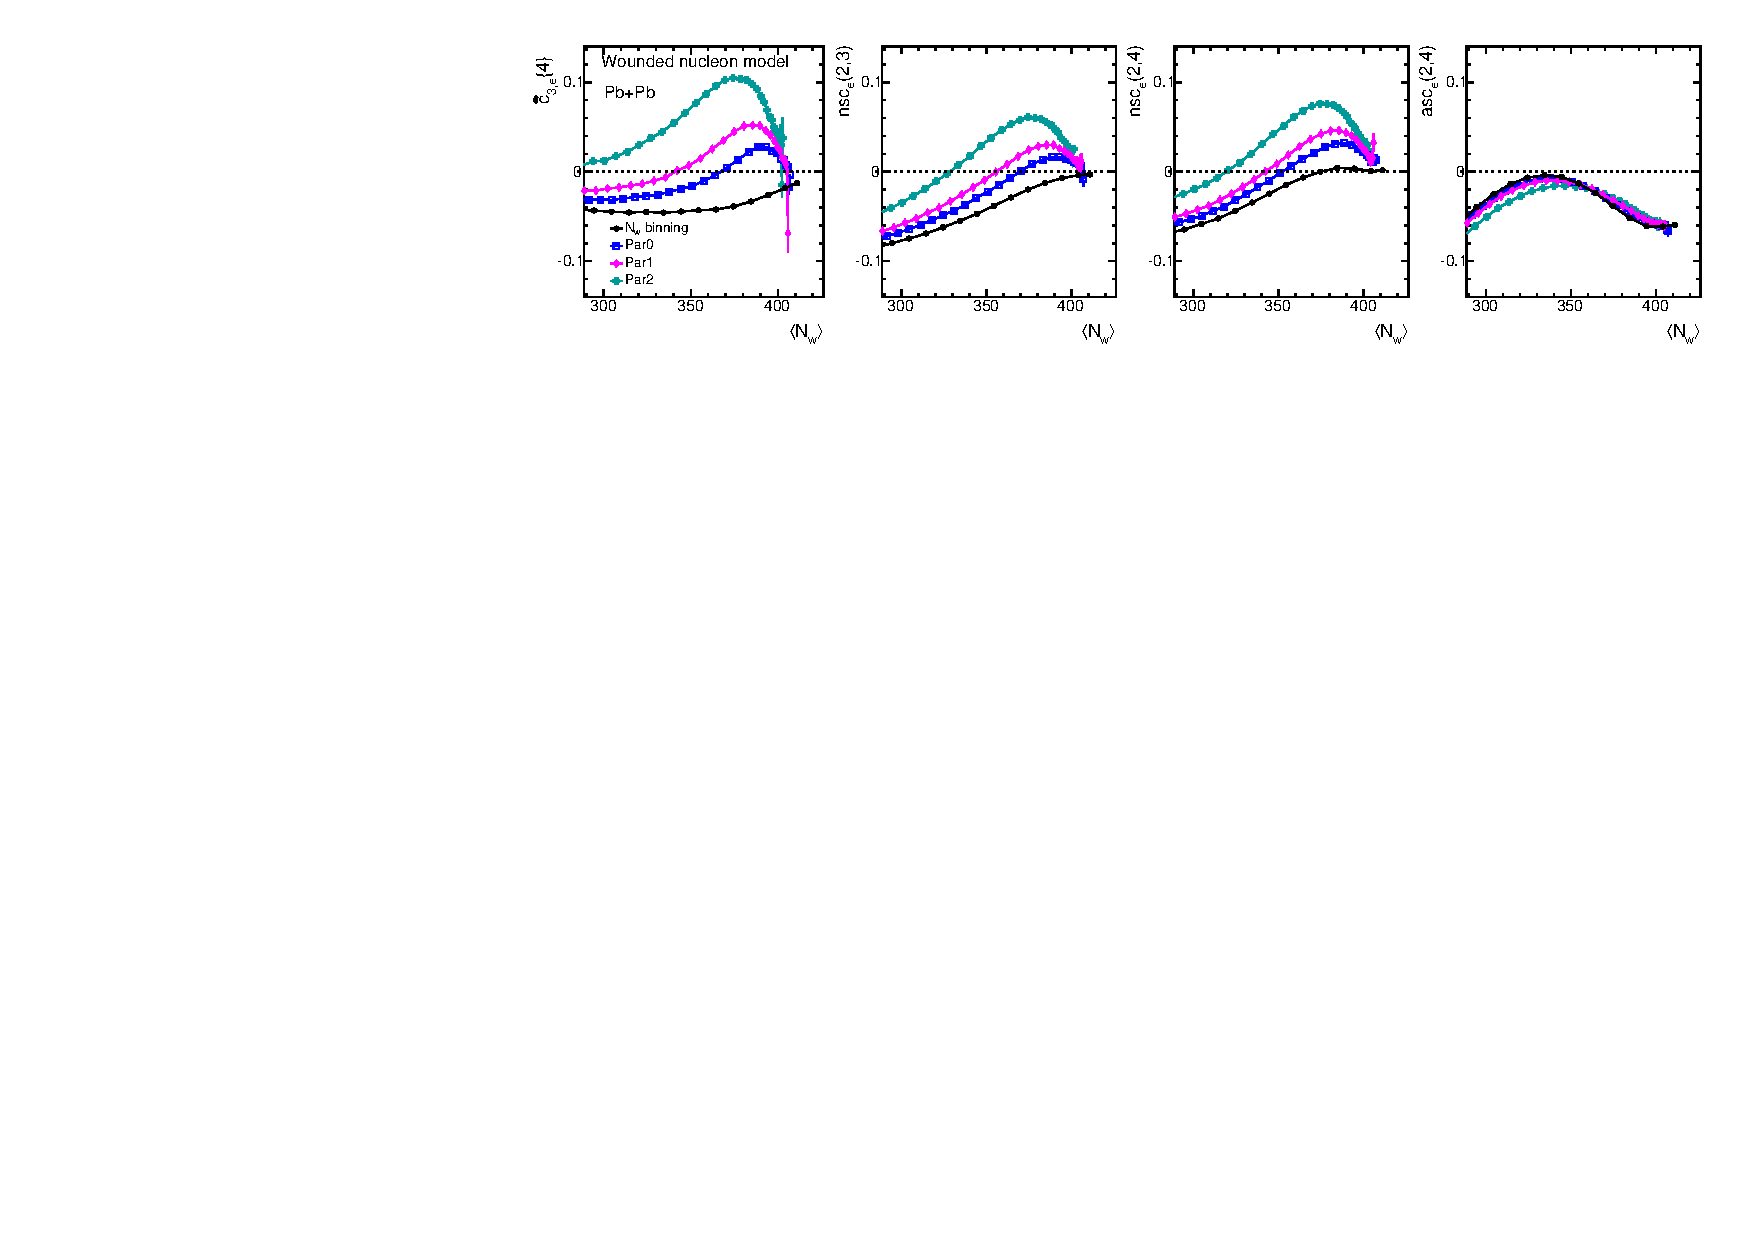
\includegraphics[width=.95\linewidth]{figs/chapter_centfluc/Glauber_others_Nw.pdf}
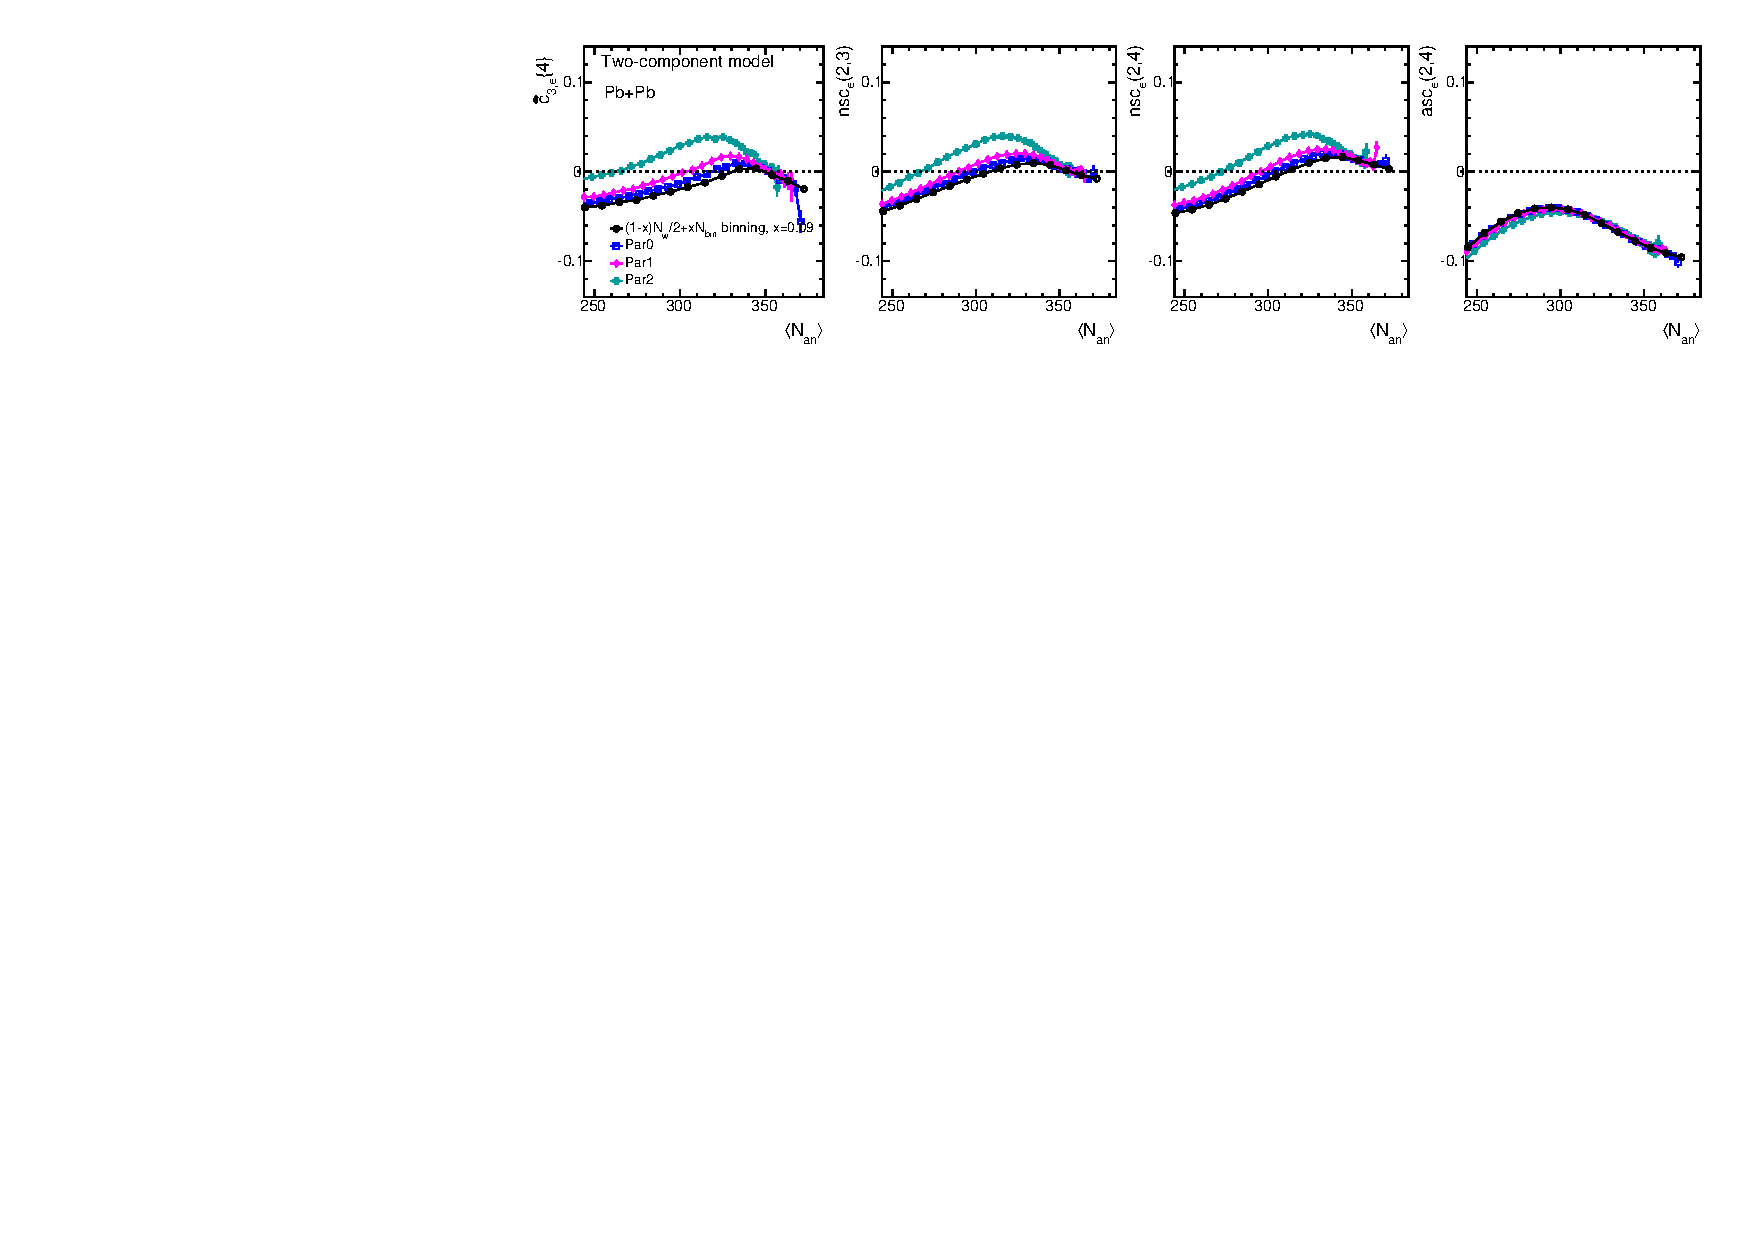
\includegraphics[width=.95\linewidth]{figs/chapter_centfluc/Glauber_others_Nan.pdf}
\caption{The normalized cumulants $nc_3\{4\}$ (left), $nsc_{2,3}\{4\}$ (second to the left), $nsc_{2,4}\{4\}$ (second to the right) and $nac_2\{3\}$ (right) for the three parameters sets for the wounded nucleon model (top row) and two-component model (bottom row). They are calculated in narrow particle multiplicity bins and then combined and mapped to an average number of $N_\text{part}$.}
\label{fig:centfluc_Glauber_others}
\end{figure}



\subsubsection{ATLAS data}
\label{sec:cent_atlas_data}

The results from various cumulant observables are presented in Section~\ref{sec:flow_cumulants_for_pvn} and Section~\ref{sec:flow_cumulants_for_pvnvm}. The cumulants are calculated using the reference event class based on $\Et$ (denoted as ${2k, \Et}$) and the results are presented as a function of centrality calculated from $\Et$. The first part discusses cumulants related to single harmonics. The second part presents correlations between two flow harmonics. The results are shown for four $\pT$ ranges and the default results are obtained using the standard cumulant method, also compared with those obtained using the three-subevent cumulant method. The last part is devoted to discussing the influence of centrality fluctuations on flow cumulants. Each cumulant observable is calculated using the $\Et$-based reference event class or $\Nchrec$-based reference event class. The results from these two reference event classes, for example $c_n\{2k, \Et\}$ and $c_n\{2k, \Nchrec\}$, are compared as a function of $\lr{\Et}$ or $\lr{\Nchrec}$. The differences are sensitive to the centrality fluctuations.



\paragraph{Flow cumulants for $p(v_n)$}
\label{sec:flow_cumulants_for_pvn}

Figure~\ref{fig:centfluc_ATLAS_nc_4pc} shows the centrality dependence of normalized four-particle cumulants $nc_2\{4\}$, $nc_3\{4\}$ and $nc_4\{4\}$ in four $\pT$ ranges from the standard method (top row) and the three-subevent method (bottom row). The advantage of using $nc_n\{4\}$ instead of $c_n\{4\}$ is that the $\pT$ dependence of the $v_n\{2\}$ is largely cancelled out, and $nc_n\{4\}$ directly reflects the shape of the $p(v_n)$ distributions~\cite{Aad:2013xma}. The results based on the three-subevent method show overall similar behavior as those for the standard cumulant method, implying that the influence of non-flow correlations are small. Therefore, the remaining discussion is focused on the standard method in the top row.

Figure~\ref{fig:centfluc_ATLAS_nc_4pc} shows that the values of $nc_2\{4\}$ and $nc_3\{4\}$ are negative in most of the centrality range. The values of $|nc_2\{4\}|$ increase and then decrease toward central collisions, while the values of $|nc_3\{4\}|$ decrease continuously toward central collisions. There centrality-dependent trends have been studied before~\cite{Aad:2014vba, Abelev:2014mda, Alver:2008zza} and were shown to be driven by the centrality dependence of the four-particle cumulants for $\epsilon_2$ and $\epsilon_3$, respectively. The normalized cumulants still show some residual dependence on $\pT$. Namely, the $|nc_2\{4\}|$ values are smaller for the higher $\pT$ particles, while the values of $|nc_3\{4\}|$ are larger for the higher $\pT$ range. Furthermore, the values of $nc_2\{4\}$ are also observed to change sign in ultra-central collisions, and the patterns of such sign change also have significant $\pT$ dependence. The behaviors of $nc_n\{4\}$ in ultra-central collisions are closely related to centrality fluctuations and are discussed further in Section~\ref{sec:dependence_on_reference_event_class_and_the_role_of_centrality_fluctuations}.

The $nc_4\{4\}$ values, as shown in the right panels of Figure~\ref{fig:centfluc_ATLAS_nc_4pc}, are negative in central collisions but change sign around $25-30\%$ centrality range. The centrality value at which the sign change occurs shifts towards more peripheral collisions as the $\pT$ of the particles increases. It is well established that the $\pmb{V}_4$ in Pb+Pb collisions contains a linear contribution associated with the initial geometry and a mode-mixing contribution from lower-order harmonics due to the nonlinear hydrodynamic response~\cite{Gardim:2011xv, Aad:2014fla, Aad:2015lwa, Qiu:2012uy, Teaney:2012ke}:
\begin{equation}
\pmb{V}_4 = \pmb{V}_{4L} + \chi_2 \pmb{V}_2^2
\end{equation}
where the linear component $\pmb{V}_{4L}$ is driven by the corresponding eccentricity $\epsilon_4$ in the initial geometry~\cite{Teaney:2010vd}, and $\chi_2$ is a constant. Previous measurements~\cite{Aad:2014fla, Aad:2015lwa} show that the $\pmb{V}_{4L}$ term dominates in central collisions, while the $\pmb{V}_2^2$ term dominates in more peripheral collisions. Therefore the sign change of $nc_4\{4\}$ could reflect an interplay between these two contributions~\cite{Giacalone:2016mdr}: in central collisions, $nc_4\{4\}$ is dominated by a negative contribution from $p(v_{4L})$, while in peripheral collisions $nc_4\{4\}$ is dominated by a positive contribution from $o(v_2^2)$. The change of the crossing point with $\pT$ suggests that the relative contributions from these two sources are also a function of $\pT$.

If the $v_n$ is driven only by the $\epsilon_n$, $p(v_n)$ should have the same shape as $p(\epsilon_n)$. On the other hand, the significant $\pT$ dependence of the $nc_n\{4\}$ in Figure~\ref{fig:centfluc_ATLAS_nc_4pc} suggests that the shape of $p(v_n)$ also changes with $\pT$. Such $\pT$-dependence behavior implies that the eccentricity fluctuations in the initial state are not the only sources for flow fluctuations. Dynamical fluctuations in the momentum space in the initial or final state may also change $p(v_n)$.

\begin{figure}[H]
\centering
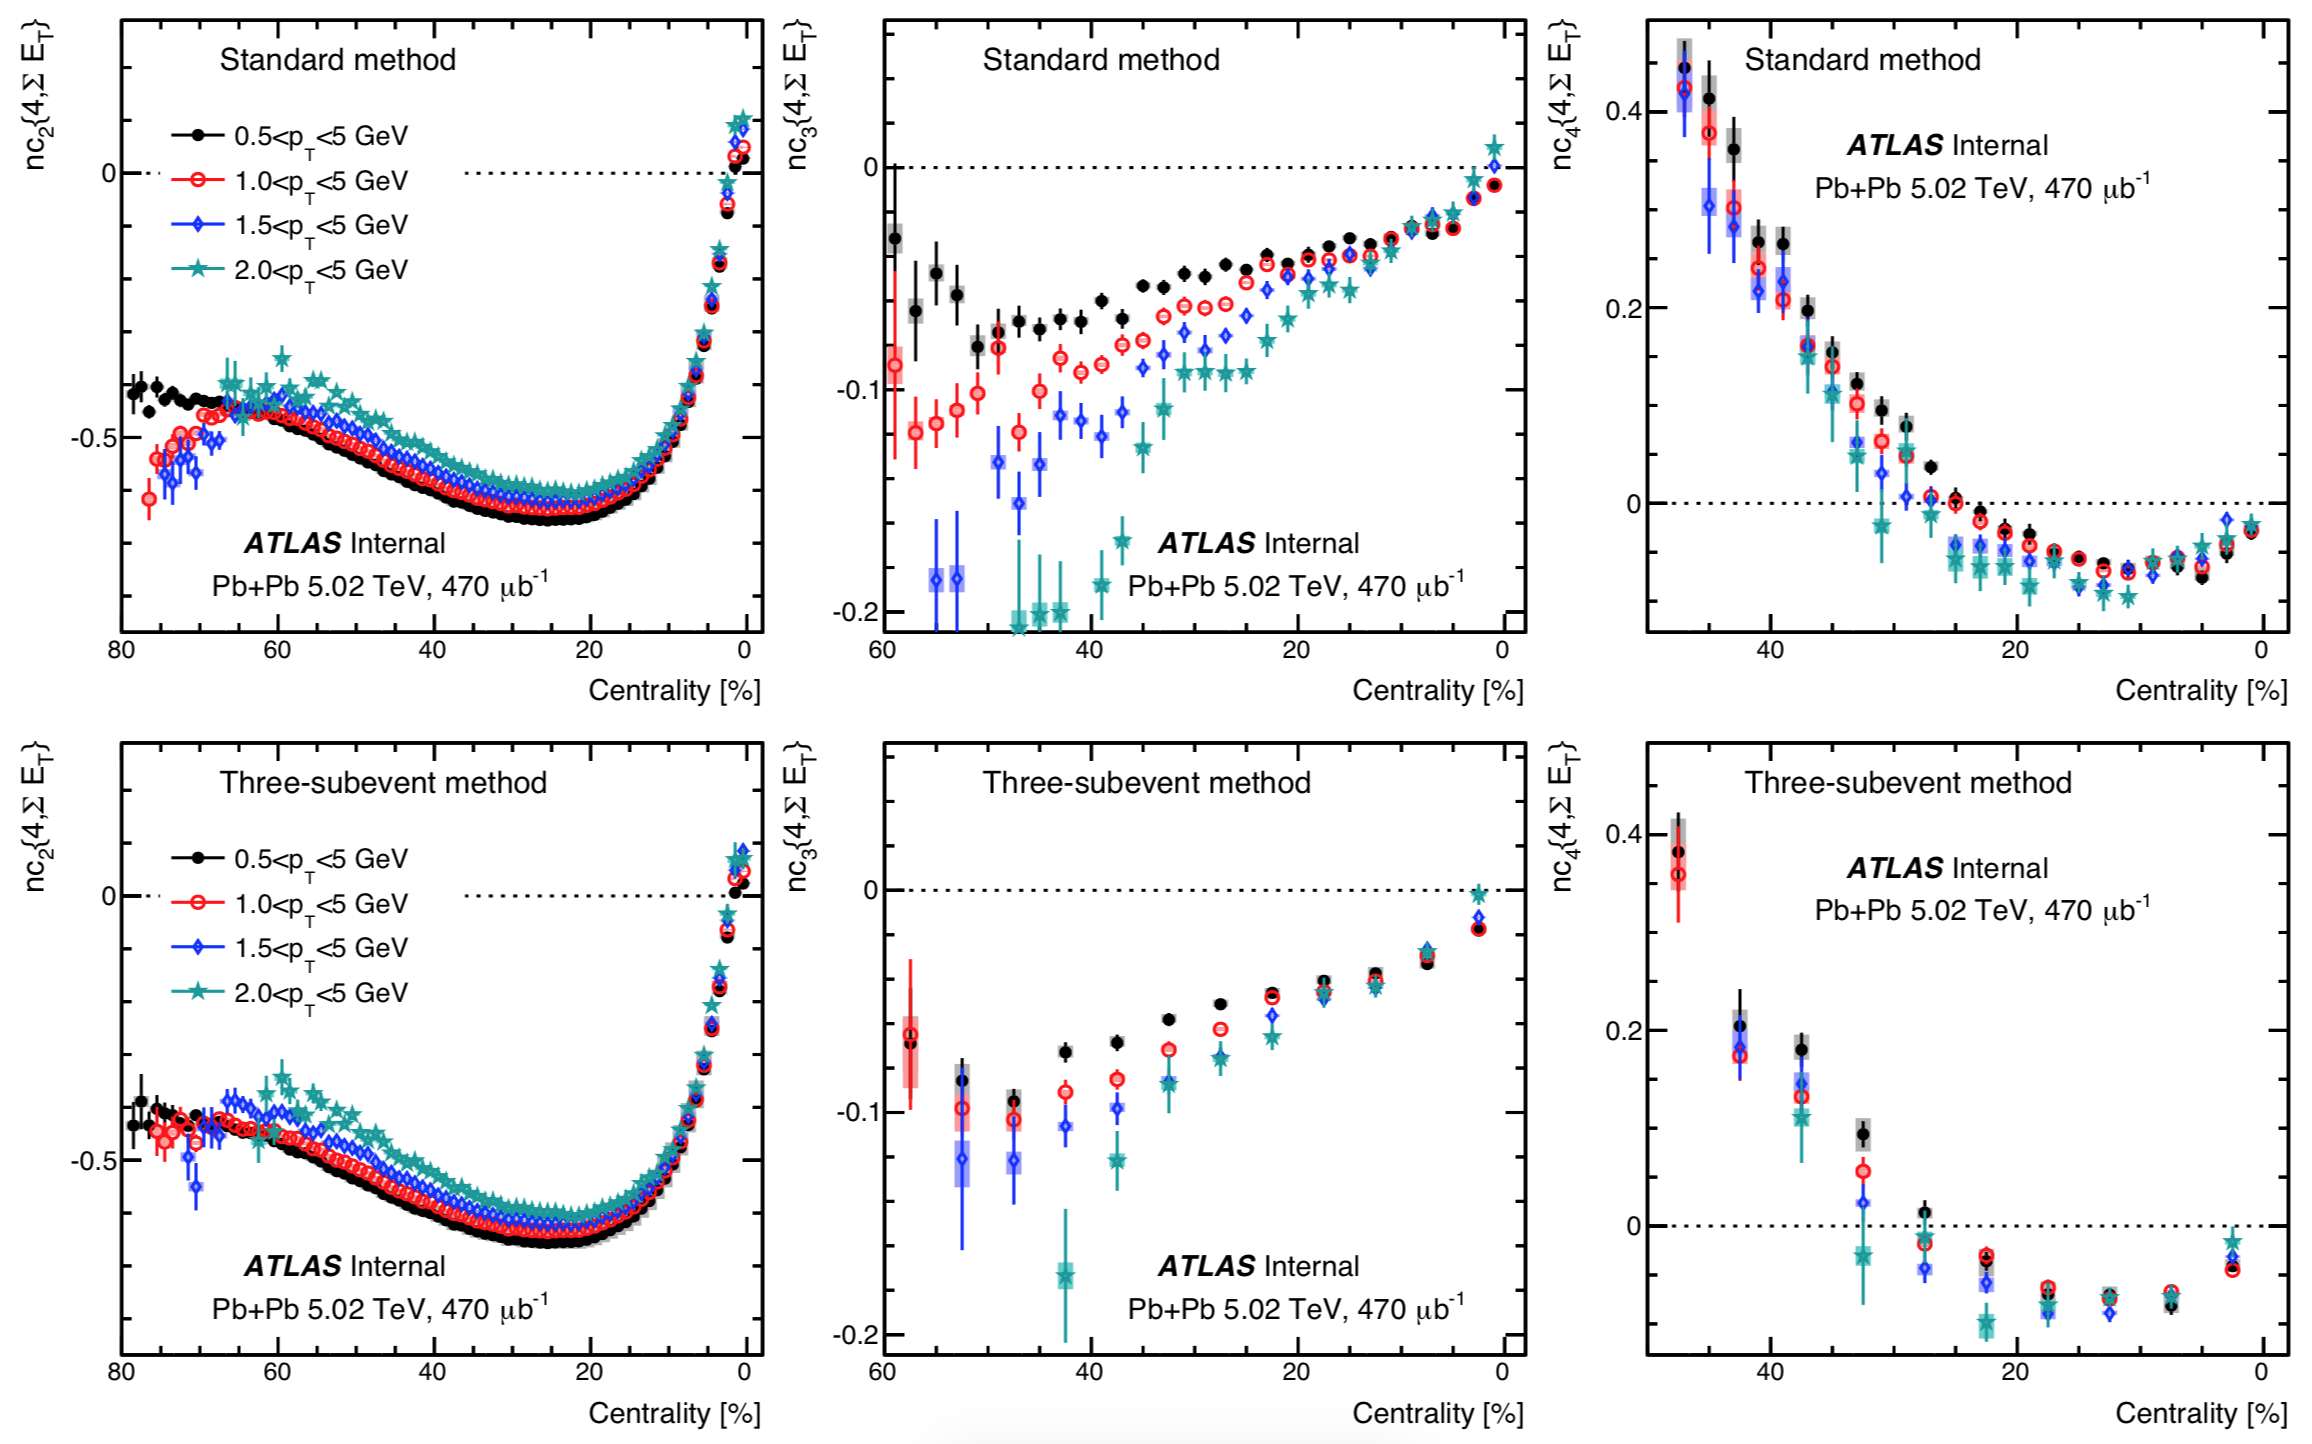
\includegraphics[width=.95\linewidth]{figs/chapter_centfluc/ATLAS_nc_4pc.png}
\caption{The centrality dependence of normalized four-particle cumulants $nc_2\{4, \Et\}$ (left), $nc_3\{4, \Et\}$ (middle) and $nc_4\{4, \Et\}$ (right) obtained with the standard method (top row) and the three-subevent method (bottom row) for four $\pT$ ranges. The error bars and shaded boxes represent the statistical and systematic uncertainties, respectively.}
\label{fig:centfluc_ATLAS_nc_4pc}
\end{figure}

Figure~\ref{fig:centfluc_ATLAS_vn_4pc_ratio} shows the cumulant ratio $v_n\{4\} / v_n\{2\}$. This ratio is directly related to the magnitude of the relative fluctuation of the $p(v_n)$ distribution. For the Gaussian fluctuation model:
\begin{equation}
\frac{v_n\{4\}}{v_n\{2\}} = \frac{v_n^0}{\sqrt{(v_n^0)^2 + \delta_n^2}}
\end{equation}
where $v_n^0$ is the mean magnitude of $v_n$ and $\delta_n$ describes the width of $v_n$ fluctuation. A ratio close to one suggest a small flow fluctuation $\delta_n \ll v_n^0$, while a ratio close to zero implies a large fluctuation $\delta_n \gg v_n^0$. The results of $v_2\{4\}/v_2\{2\}$ imply that flow fluctuations are small relative to the $v_n^0$, but become larger in the most central collisions. The results of $v_3\{4\} / v_3\{2\}$ suggest that the relative fluctuation of $p(v_3)$ grows gradually from peripheral to central collisions. The values of $v_4\{4\} / v_4\{2\}$ are around $0.4-0.5$ in $0-20\%$ centrality range, comparable or slightly larger than the values of $v_3\{4\} / v_3\{2\}$. In peripheral collisions, $v_4\{4\} / v_4\{2\}$ is negative and its magnitude increases and reaches minus one in very peripheral collisions, suggesting a significant departure of $p(v_4)$ from Gaussian. The large statistical uncertainties around the sign change region is due to the divergence in the first derivative of the function $\sqrt[4]{|nc_4\{4\}|}$ around $nc_4\{4\}=0$.

\begin{figure}[H]
\centering
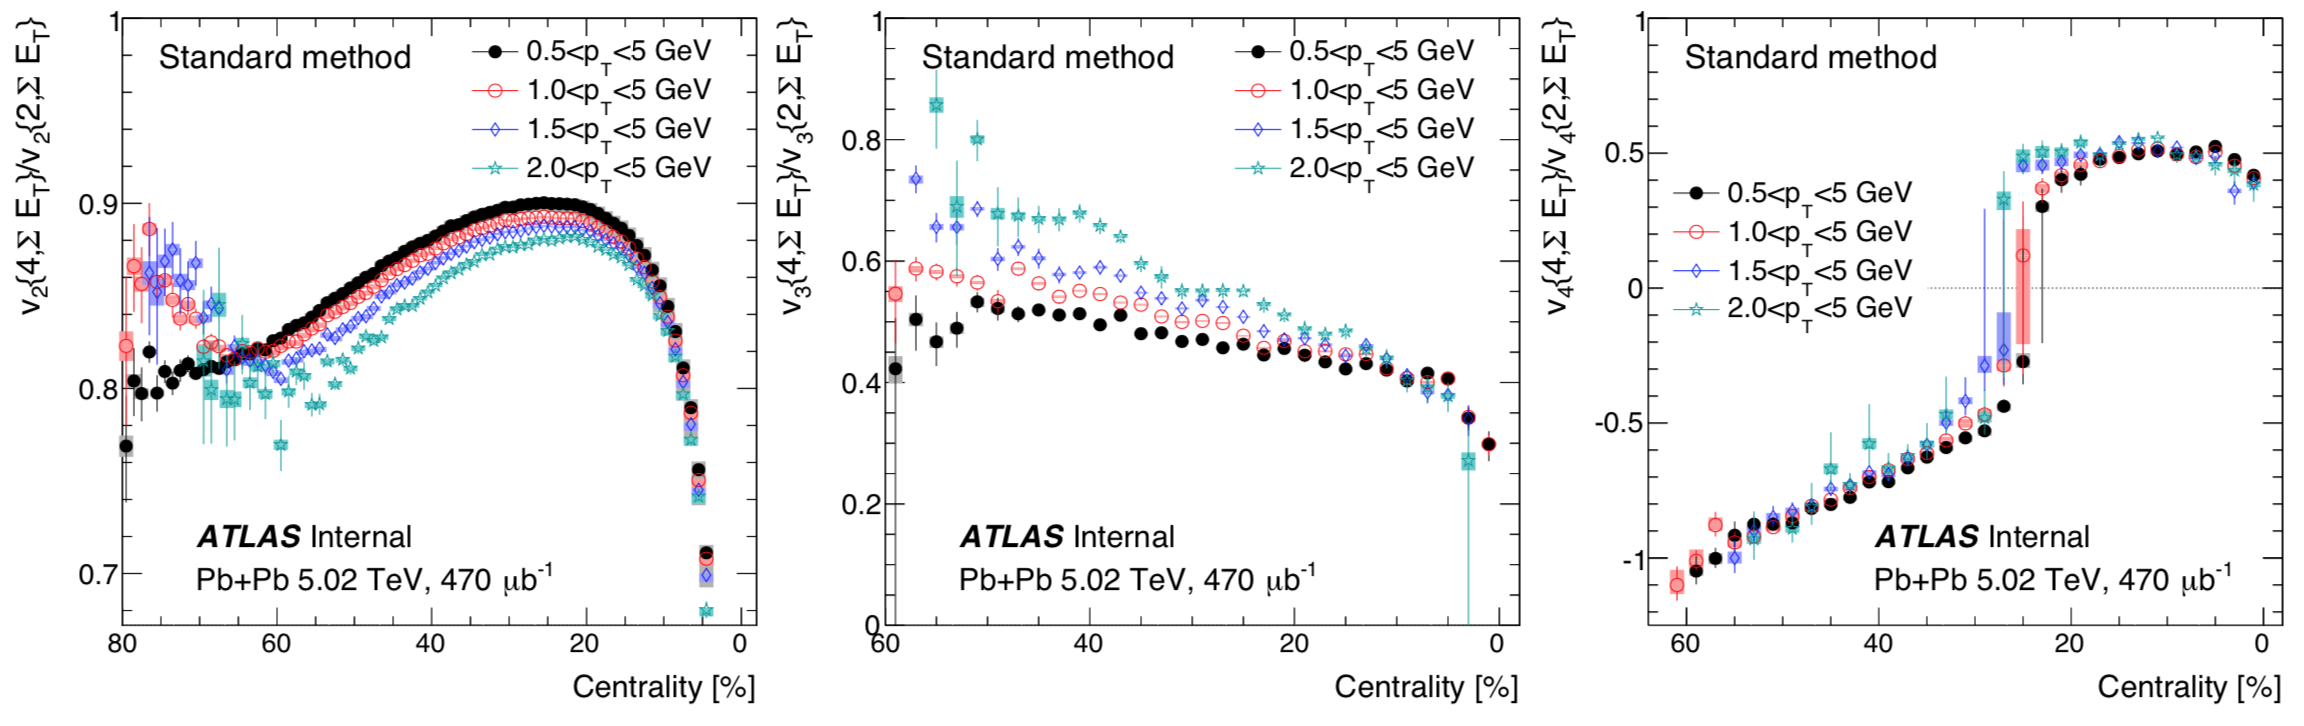
\includegraphics[width=.95\linewidth]{figs/chapter_centfluc/ATLAS_vn_4pc_ratio.png}
\caption{The centrality dependence of cumulant ratios $v_n\{4, \Et\} / v_n\{2, \Et\}$ for $n=2$ (left), $n=3$ (middle) and $n=4$ (right) for four $\pT$ ranges. The error bars and shaded boxes represent the statistical and systematic uncertainties, respectively.}
\label{fig:centfluc_ATLAS_vn_4pc_ratio}
\end{figure}

Figure~\ref{fig:centfluc_ATLAS_vn_6pc_ratio} shows the centrality dependence of normalized six-particle cumulants $nc_2\{6\}$, $nc_3\{6\}$ and $nc_4\{6\}$. These quantities are directly related to the cumulant ratios $v_n\{6\} / v_n\{2\}$. The values of $nc_2\{6\}$ are positive over most of the centrality range, but reach zero in ultra-central collisions. The centrality dependence of $|nc_2\{6\}|$ is very similar to that for $|nc_2\{4\}|$ in the left panel of Figure~\ref{fig:centfluc_ATLAS_nc_4pc}. The values of $nc_3\{6\}$ and $nc_4\{6\}$ are much smaller and have larger statistical uncertainties. Therefore, only the results from the two $\pT$ ranges with lower $\pT$ thresholds, which have the best statistical precision, are shown. The values are smaller than 0.005 and 0.01 for $nc_3\{6\}$ and $nc_4\{6\}$, which correspond to an upper limit of $|v_3\{6\} / v_3\{2\}| \le 0.38$ and $|v_4\{6\} / v_4\{2\}| \le 0.46$, respectively.

\begin{figure}[H]
\centering
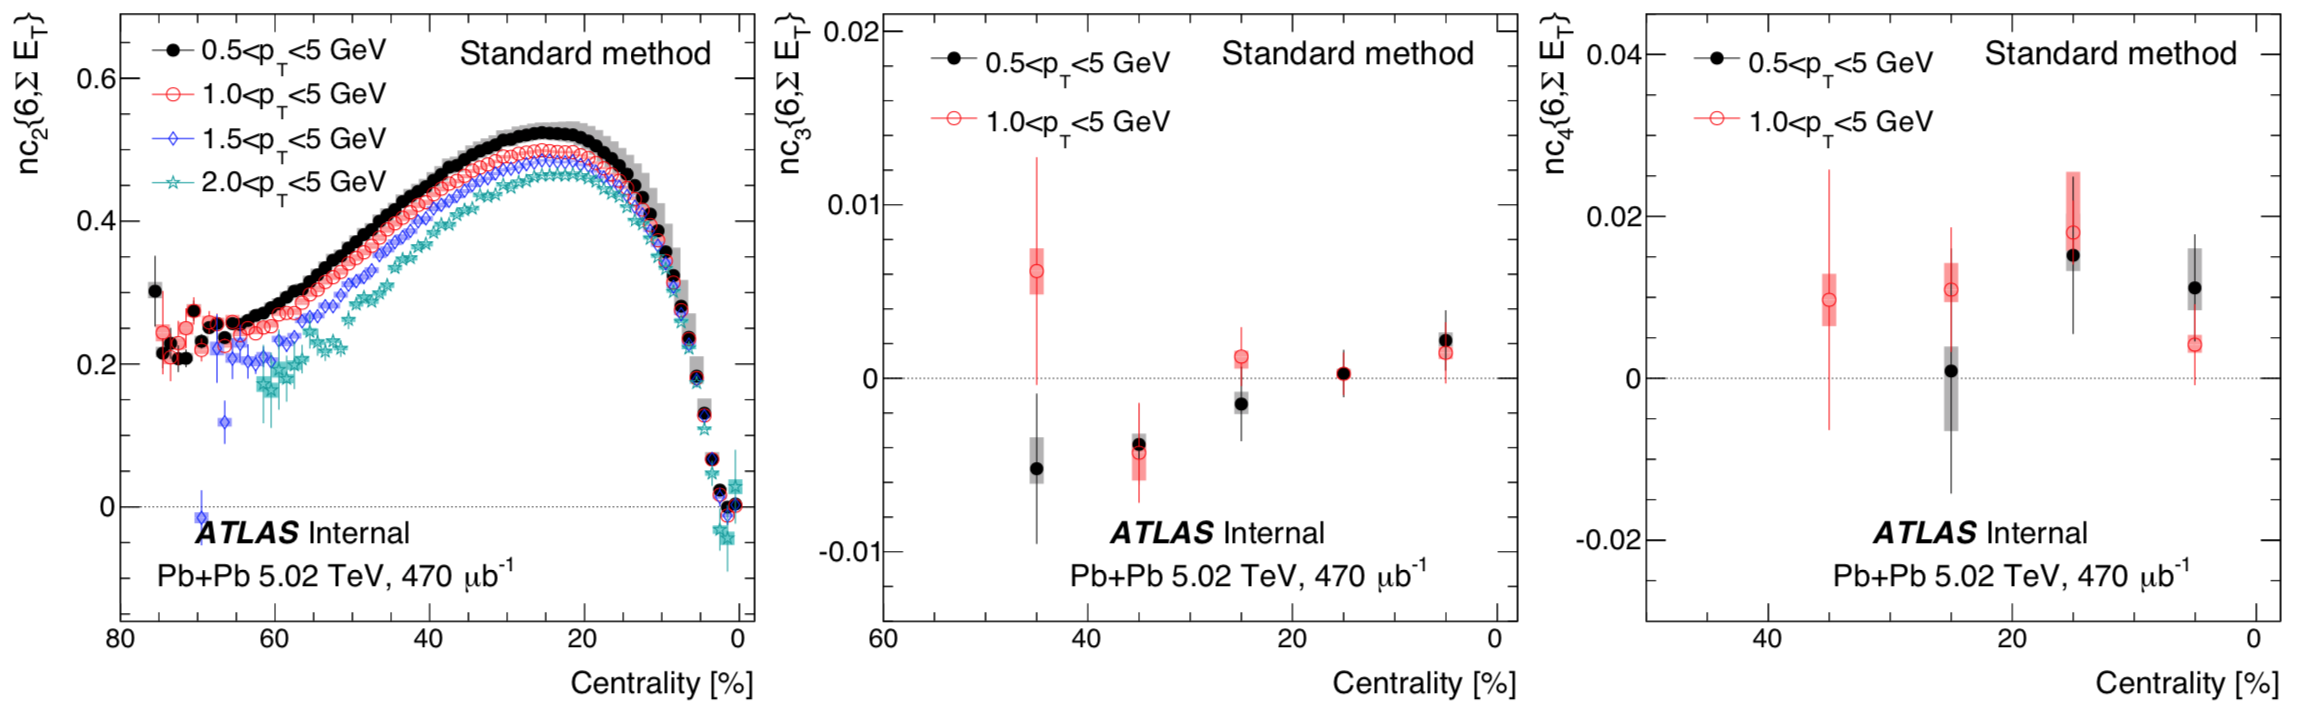
\includegraphics[width=.95\linewidth]{figs/chapter_centfluc/ATLAS_vn_6pc_ratio.png}
\caption{The centrality dependence of normalized six-particle cumulants $nc_2\{6, \Et\}$ (left), $nc_3\{6, \Et\}$ (middle) and $nc_4\{6, \Et\}$ (right) obtained with the standard method (top row) and the three-subevent method (bottom row) for four $\pT$ ranges. The error bars and shaded boxes represent the statistical and systematic uncertainties, respectively.}
\label{fig:centfluc_ATLAS_vn_6pc_ratio}
\end{figure}

From the measured $nc_2\{6\}$ and $nc_2\{4\}$, the ratio of six-particle cumulant and four-particle cumulant $v_2\{6\} / v_2\{4\}$ can be obtained. The results are shown in Figure~\ref{fig:centfluc_ATLAS_v2_64pc_ratio}. For the Gaussian fluctuation model, this ratio is expected to be one. The apparent deviation of the ratio from one suggests non-Gaussianity of $p(v_2)$ over a broad centrality range. The results for different $\pT$ ranges are close to each other, but nevertheless show systematic and centrality dependence differences. In general, the results from higher $\pT$ are larger in central collisions and smaller in peripheral collisions than those from the lower $\pT$.

\begin{figure}[H]
\centering
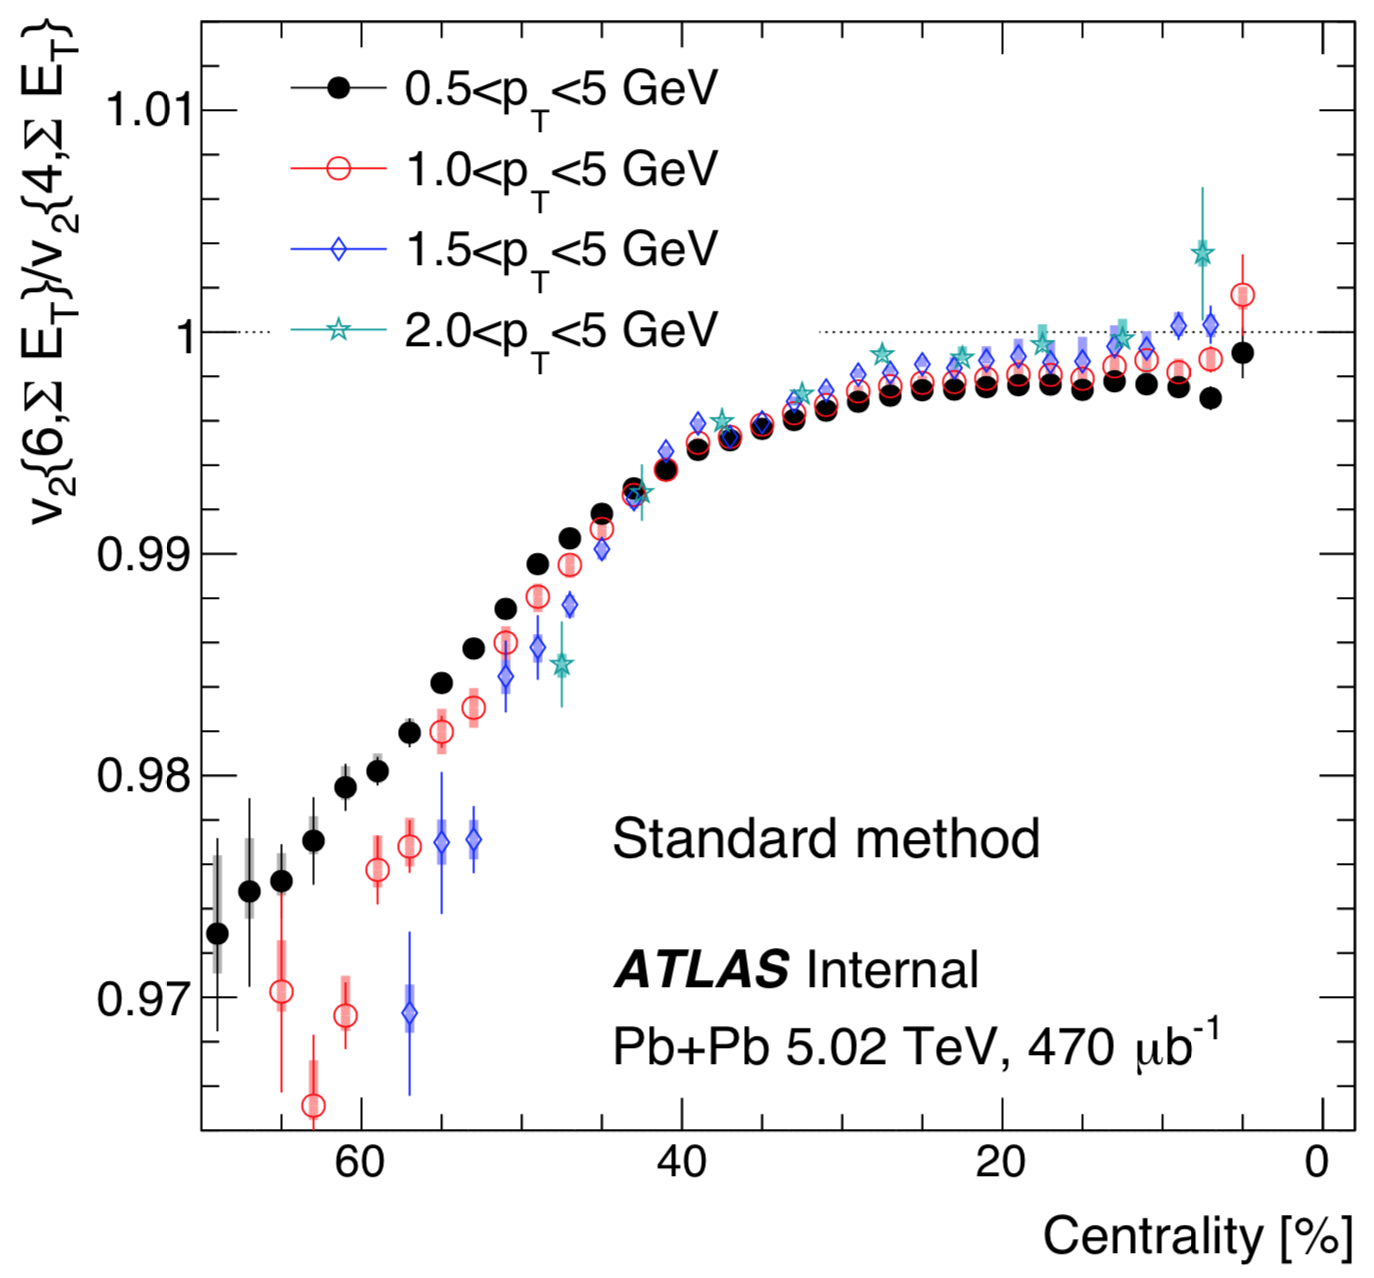
\includegraphics[width=.475\linewidth]{figs/chapter_centfluc/ATLAS_v2_64pc_ratio.png}
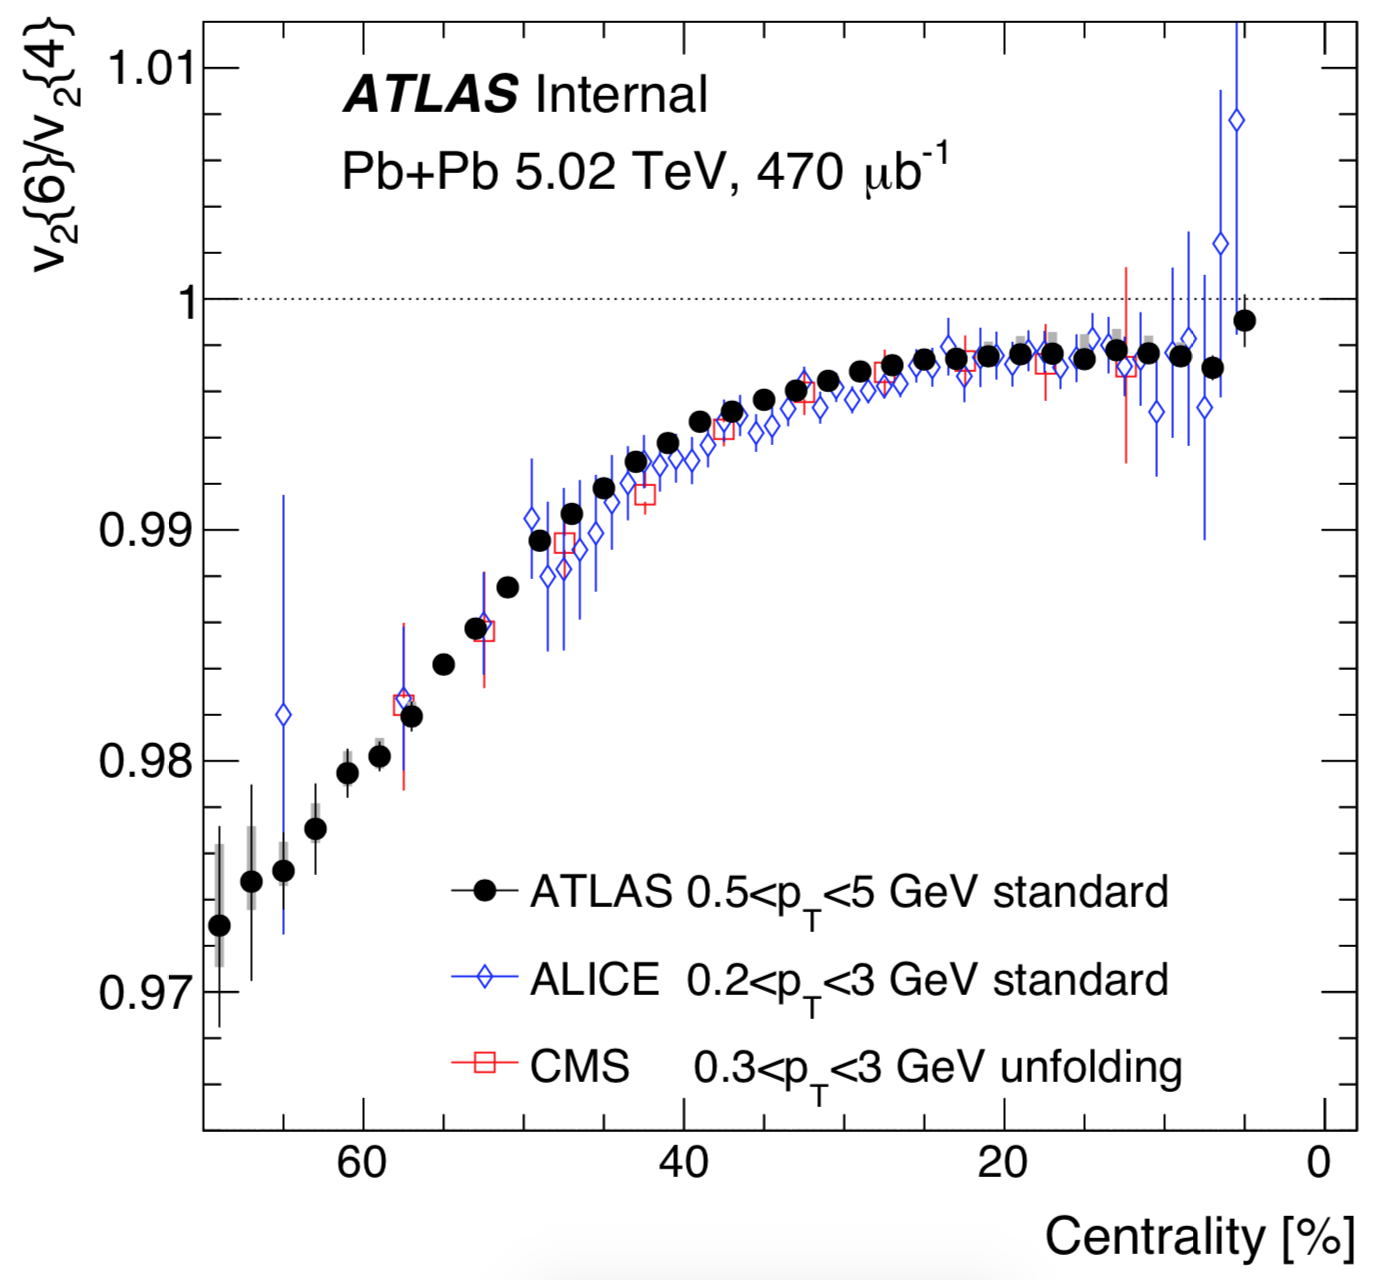
\includegraphics[width=.475\linewidth]{figs/chapter_centfluc/ATLAS_v2_64pc_ratio_comp.png}
\caption{The centrality dependence of cumulant ratio $v_2\{6, \Et\} / v_2\{4, \Et\}$ for four $\pT$ ranges (left), and compared with ALICE and CMS published results (right). The error bars and shaded boxes represent the statistical and systematic uncertainties, respectively.}
\label{fig:centfluc_ATLAS_v2_64pc_ratio}
\end{figure}

The multi-particle correlations are also performed to obtain cumulants for dipolar flow $v_1$. Top row of Figure~\ref{fig:centfluc_ATLAS_v1_4pc} shows the centrality dependence of $c_1\{4\}$ in several $\pT$ ranges, obtained from the reference event class based on $\Et$. In the hydrodynamical picture, $c_1\{4\}$ is sensitive to event-by-event fluctuations of the dipolar eccentricity $\epsilon_1$ associated with initial-state geometry. The uncertainty for this measurement is large since both $\lr{\lr{corr_1\{4\}}}$ and $\lr{\lr{corr_1\{2\}}}$ contain a significant contribution from global momentum conservation effects~\cite{ATLAS:2012at, Borghini:2002mv}. This contribution cancels for $c_1\{4\}$, but leads to a large statistical uncertainty. A negative $c_1\{4\}$ for $\pT>1.5$ GeV is observed in both the standard and three-subevent cumulant methods, which reflects the event-by-event fluctuations of the dipolar eccentricity.

Previously, ATLAS measured $v_1$ using two-particle correlation method in Pb+Pb collision at 2.76 TeV, where an explicit procedure is employed to subtract the global momentum conservation effects~\cite{ATLAS:2012at}. The $v_1\{2\}$ was observed to be negative at low $\pT$, changes sign at $\pT \approx 1.2$ GeV, and increase quickly towards higher $\pT$. Therefore, it is naturally expected that a $c_1\{4\}$ signal is larger and easier to measure at higher $\pT$. Bottom panels of Figure~\ref{fig:centfluc_ATLAS_v1_4pc} shows the $v_1\{4\}$ calculated from $c_1\{4\}$ for the two highest $\pT$ ranges. The $v_1\{4\}$ values increase with $\pT$ and toward more peripheral collisions, and are in the range of $0.02-0.04$ for $2.0<\pT<5.0$ GeV.

\begin{figure}[H]
\centering
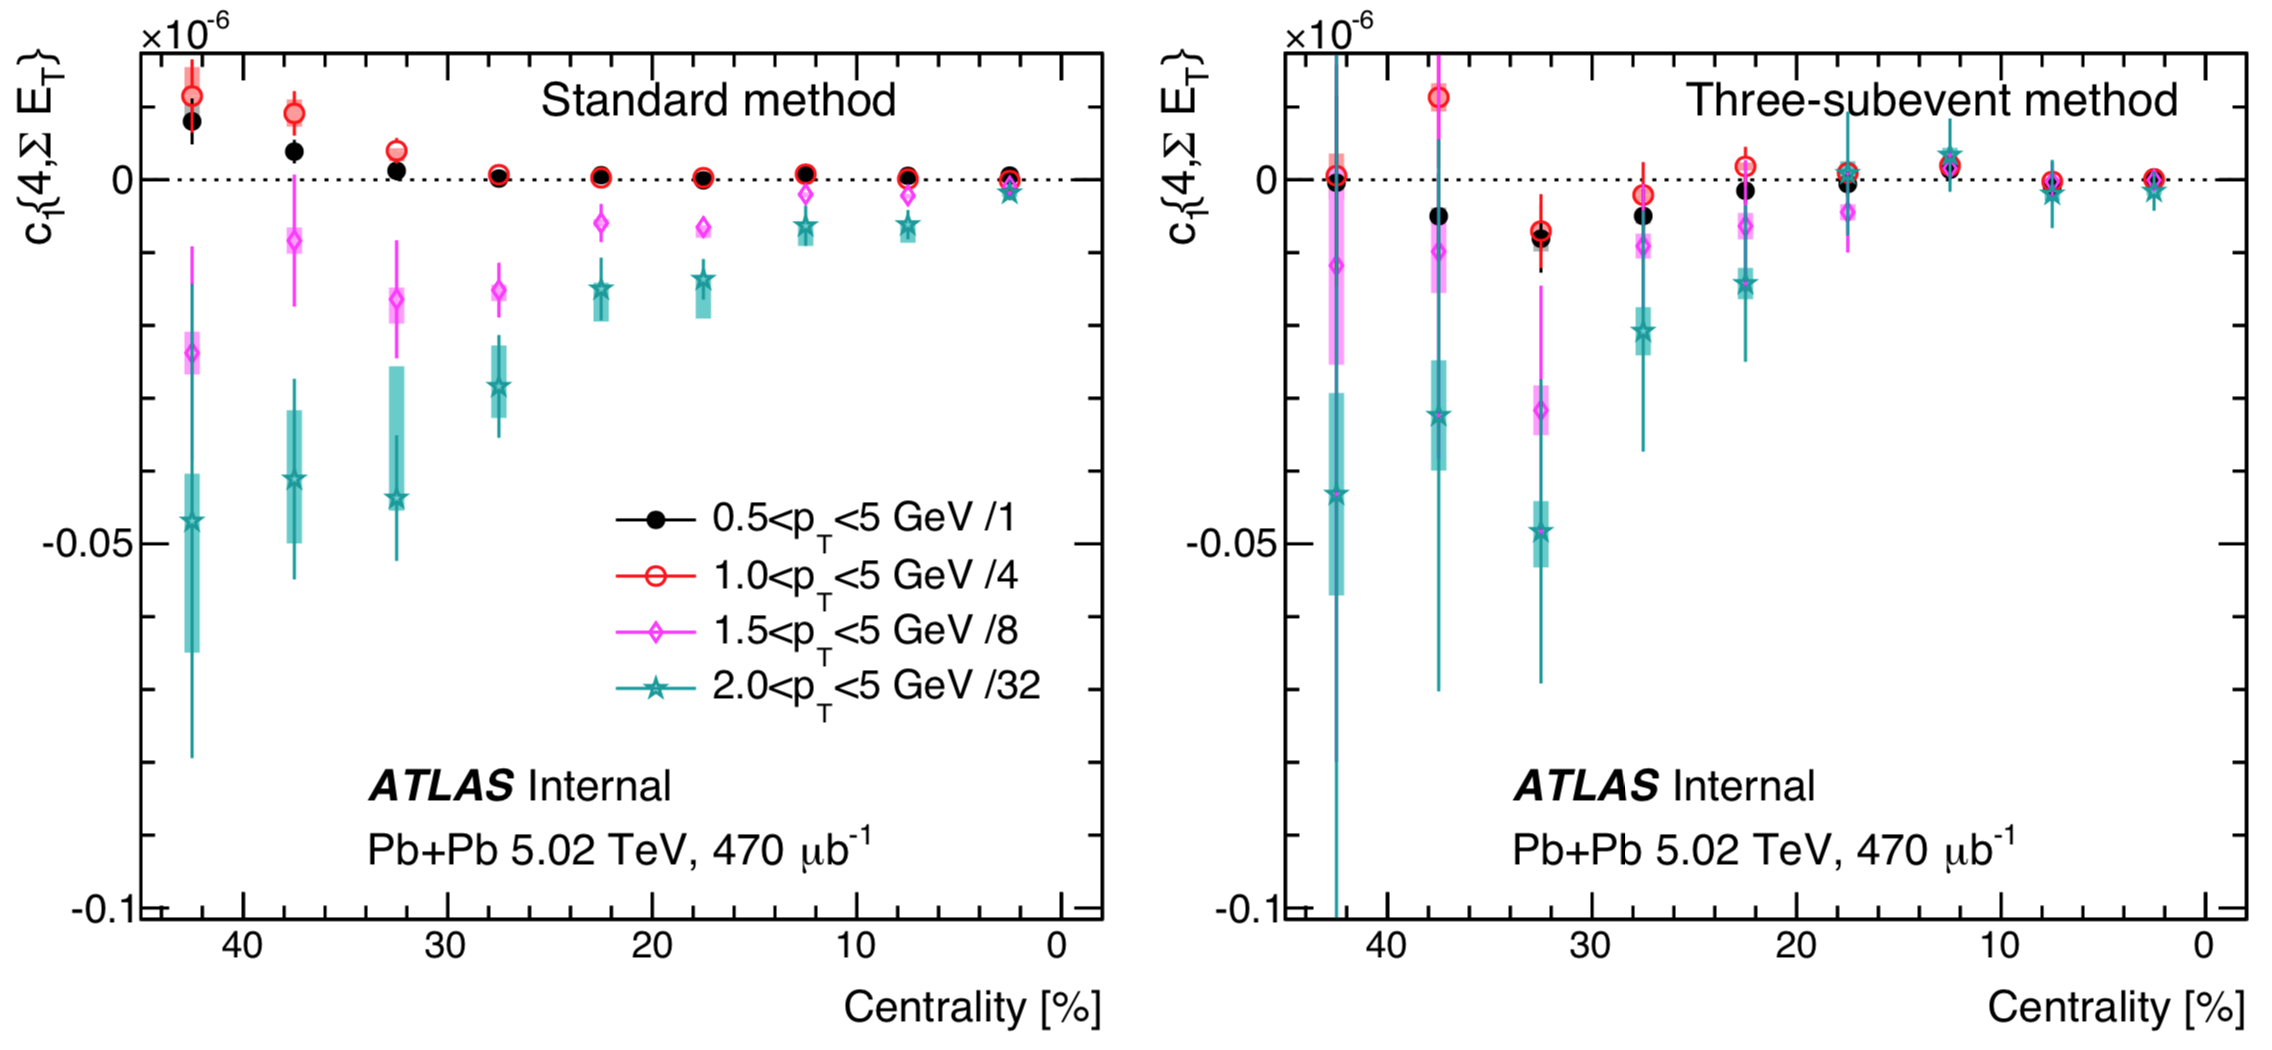
\includegraphics[width=.95\linewidth]{figs/chapter_centfluc/ATLAS_c1_4pc.png}
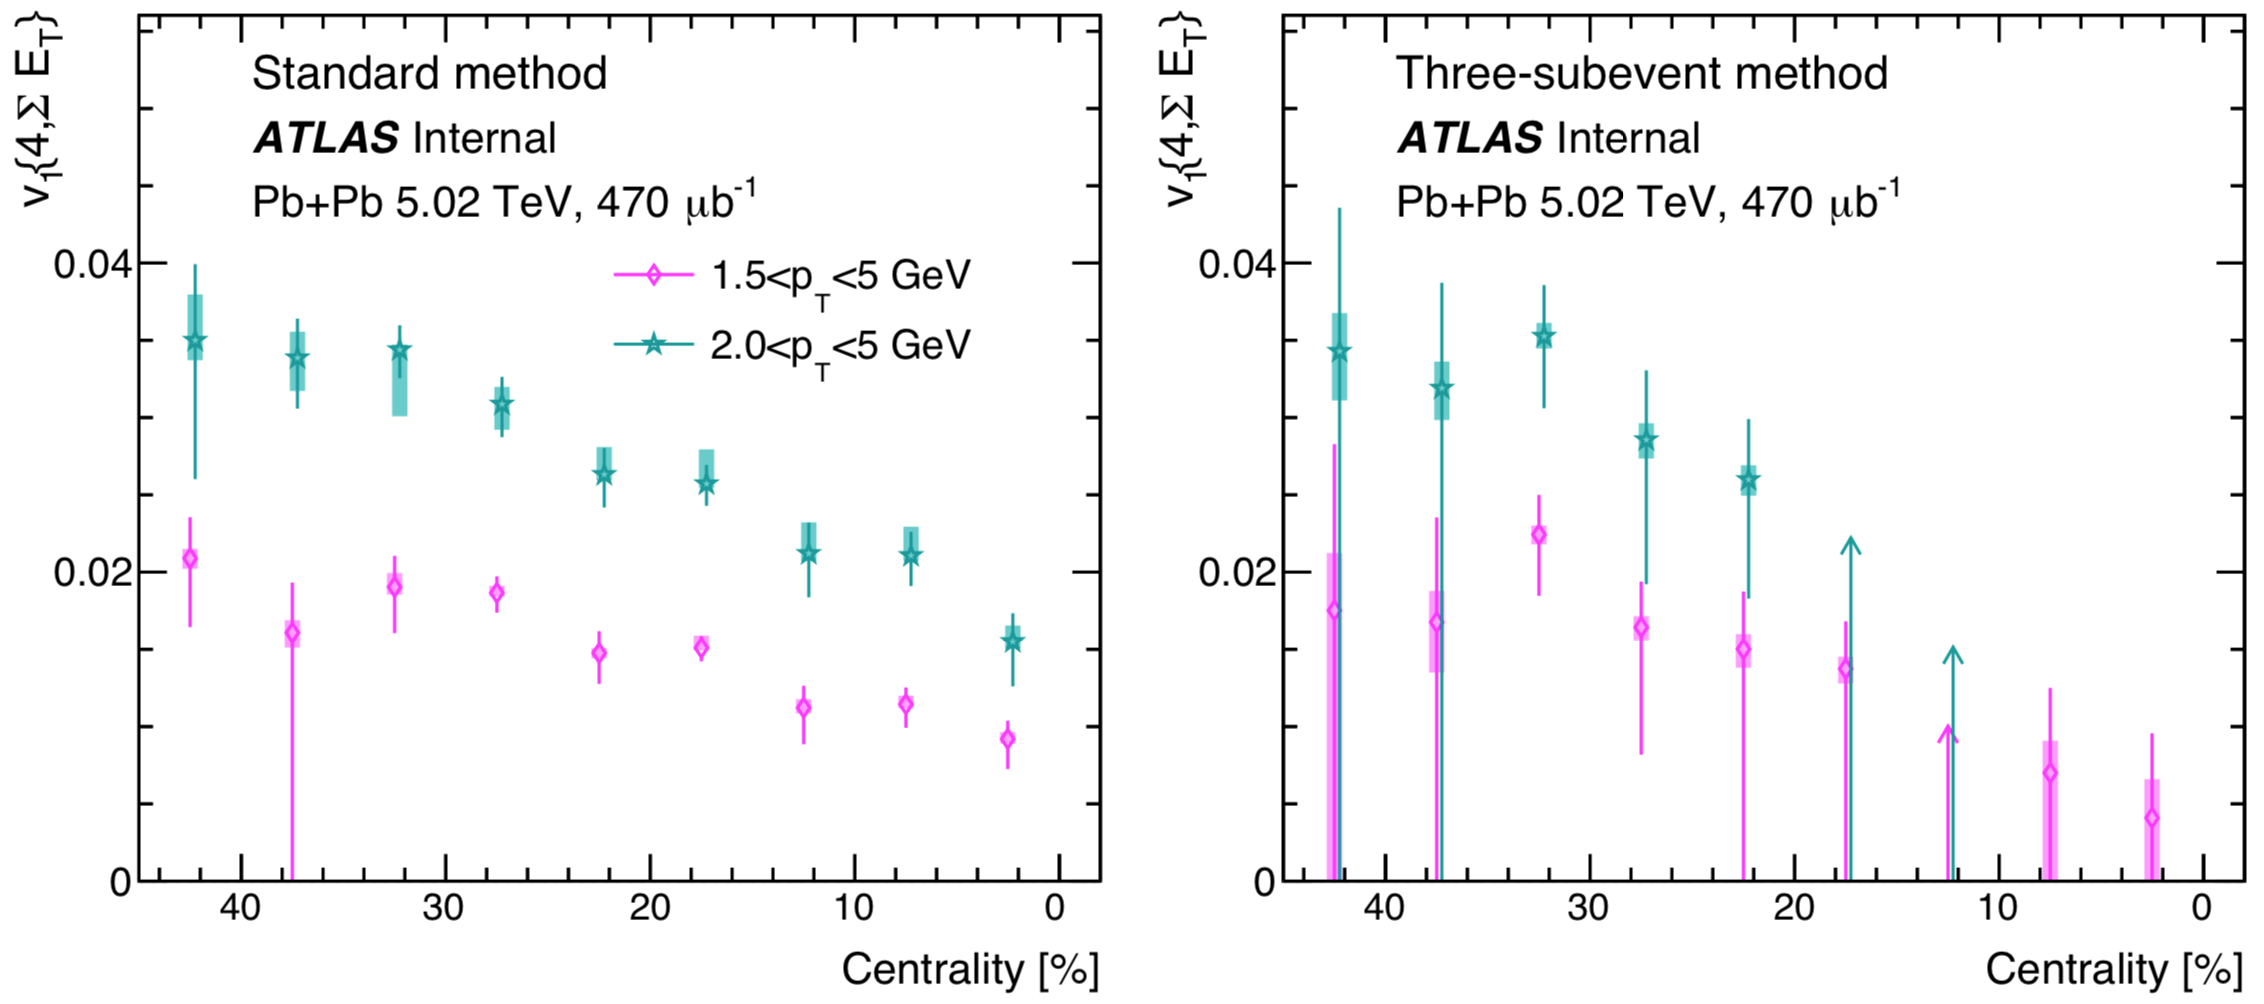
\includegraphics[width=.95\linewidth]{figs/chapter_centfluc/ATLAS_v1_4pc.png}
\caption{The centrality dependence of $c_1\{4\}$ (top row) and $v_1\{4\}$ (bottom row) calculated for charged particles in several $\pT$ ranges with the standard method (left) and three-subevent method (right). The error bars and shaded boxes represent the statistical and systematic uncertainties, respectively. The data for each $\pT$ ranges are scaled by a constant factor indicated in the legend for the purpose of presentation.}
\label{fig:centfluc_ATLAS_v1_4pc}
\end{figure}




\paragraph{Flow cumulants for $p(v_n, v_m)$}
\label{sec:flow_cumulants_for_pvnvm}

The correlation between flow harmonics of different order is studied using the four-particle normalized symmetric cumulants, $nsc_{2,3}\{4\}$ and $nsc_{2,4}\{4\}$, and the three-particle normalized asymmetric cumulants $nac_2\{3\}$. Figure~\ref{fig:centfluc_ATLAS_nsc23} in several $\pT$ ranges, which probes the correlation between $v_2$ and $v_3$. The $nsc_{2,3}\{4\}$ is negative in most of the centrality range, indicating an anti-correlation between $v_2$ and $v_3$. The strength of the anti-correlation has significant $\pT$ dependence. For higher $\pT$ particles, the anti-correlation is stronger in peripheral collisions and weaker in central collisions. In the ultra-central collisions, the $nsc_{2,3}\{4\}$ changes sign and becomes positive. This positive correlation is related to centrality fluctuations and is discussed further in Section~\ref{sec:dependence_on_reference_event_class_and_the_role_of_centrality_fluctuations}. The overall centrality and $\pT$ dependence behavior are also found to be similar between the standard cumulant method and the three-subevent cumulant method, which suggests that these features are not caused by non-flow correlations.

\begin{figure}[H]
\centering
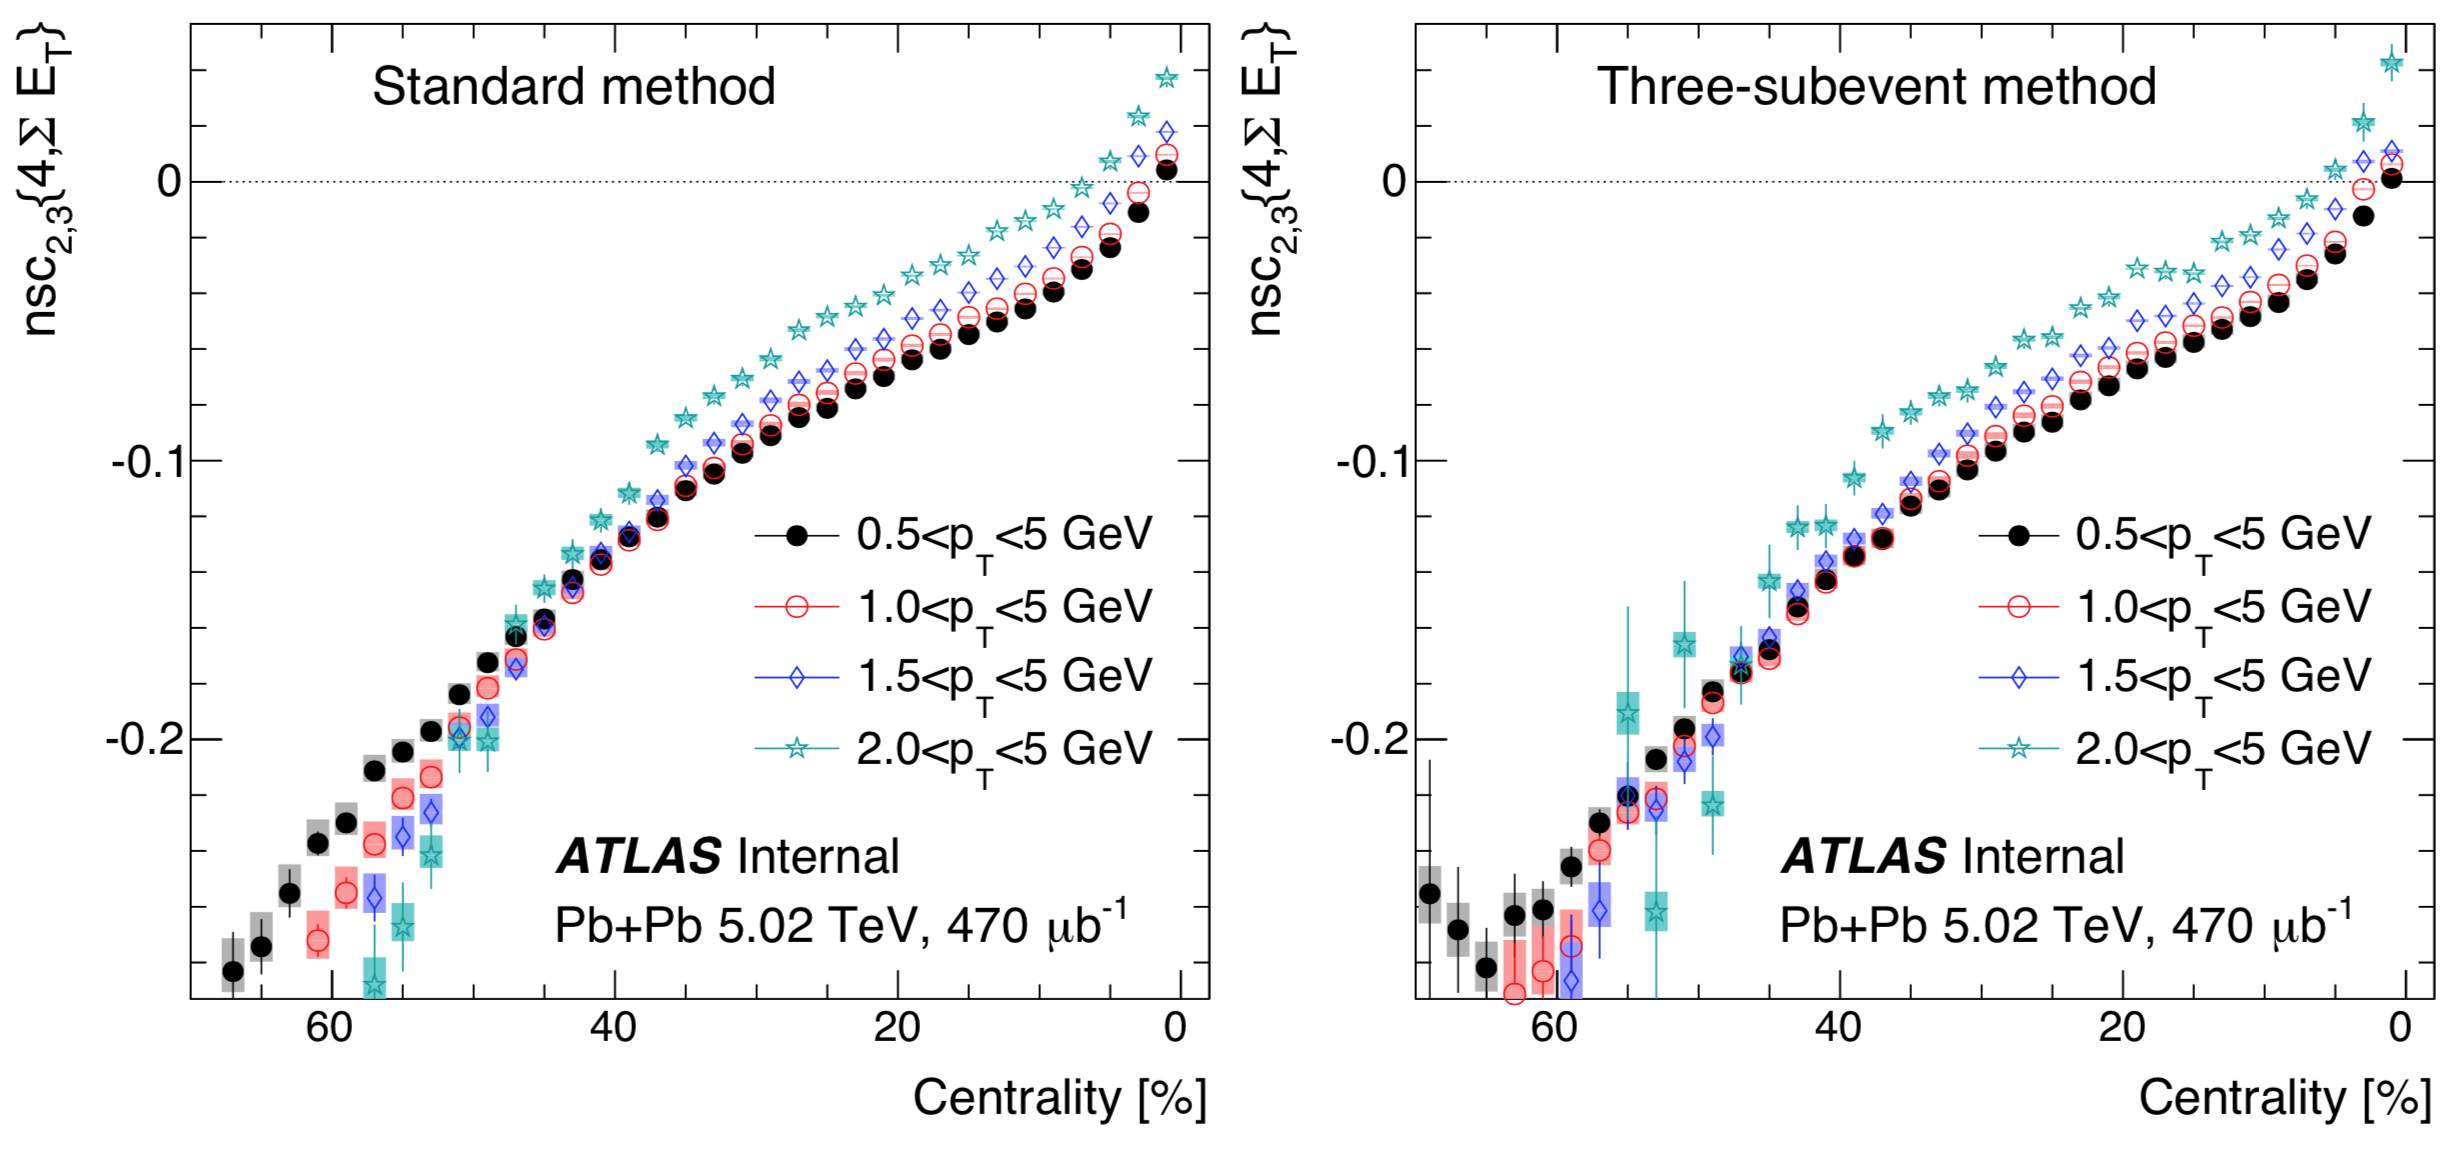
\includegraphics[width=.95\linewidth]{figs/chapter_centfluc/ATLAS_nsc23.png}
\caption{The centrality dependence of $nsc_{2,3}\{4\}$ calculated for charged particles in four $\pT$ ranges with the standard method (left) and three-subevent method (right). The error bars and shaded boxes represent the statistical and systematic uncertainties, respectively.}
\label{fig:centfluc_ATLAS_nsc23}
\end{figure}

Figure~\ref{fig:centfluc_ATLAS_nsc24} shows the centrality dependence of $nsc_{2,4}\{4\}$ in several $\pT$ ranges, which probes the correlation between $v_2$ and $v_4$. The $nsc_{2,4}\{4\}$ is positive over the entire centrality range, indicating a positive correlation between the $v_2$ and $v_4$. The signal is very small in central collisions, but increases rapidly towards peripheral collisions. The correlations are similar between different $\pT$ ranges in central collisions, but are slightly weaker for higher $\pT$ particles in mid-central collisions, a behavior also predicted by hydrodynamic models~\cite{Niemi:2012aj, Zhu:2016puf}. Comparing to the three-subevent method, the $nsc_{2,4}\{4\}$ values from the standard method have better statistical precision but slightly higher values in peripheral collisions, indicating that the non-flow effects may become significant for events beyond $60\%$ centrality.

\begin{figure}[H]
\centering
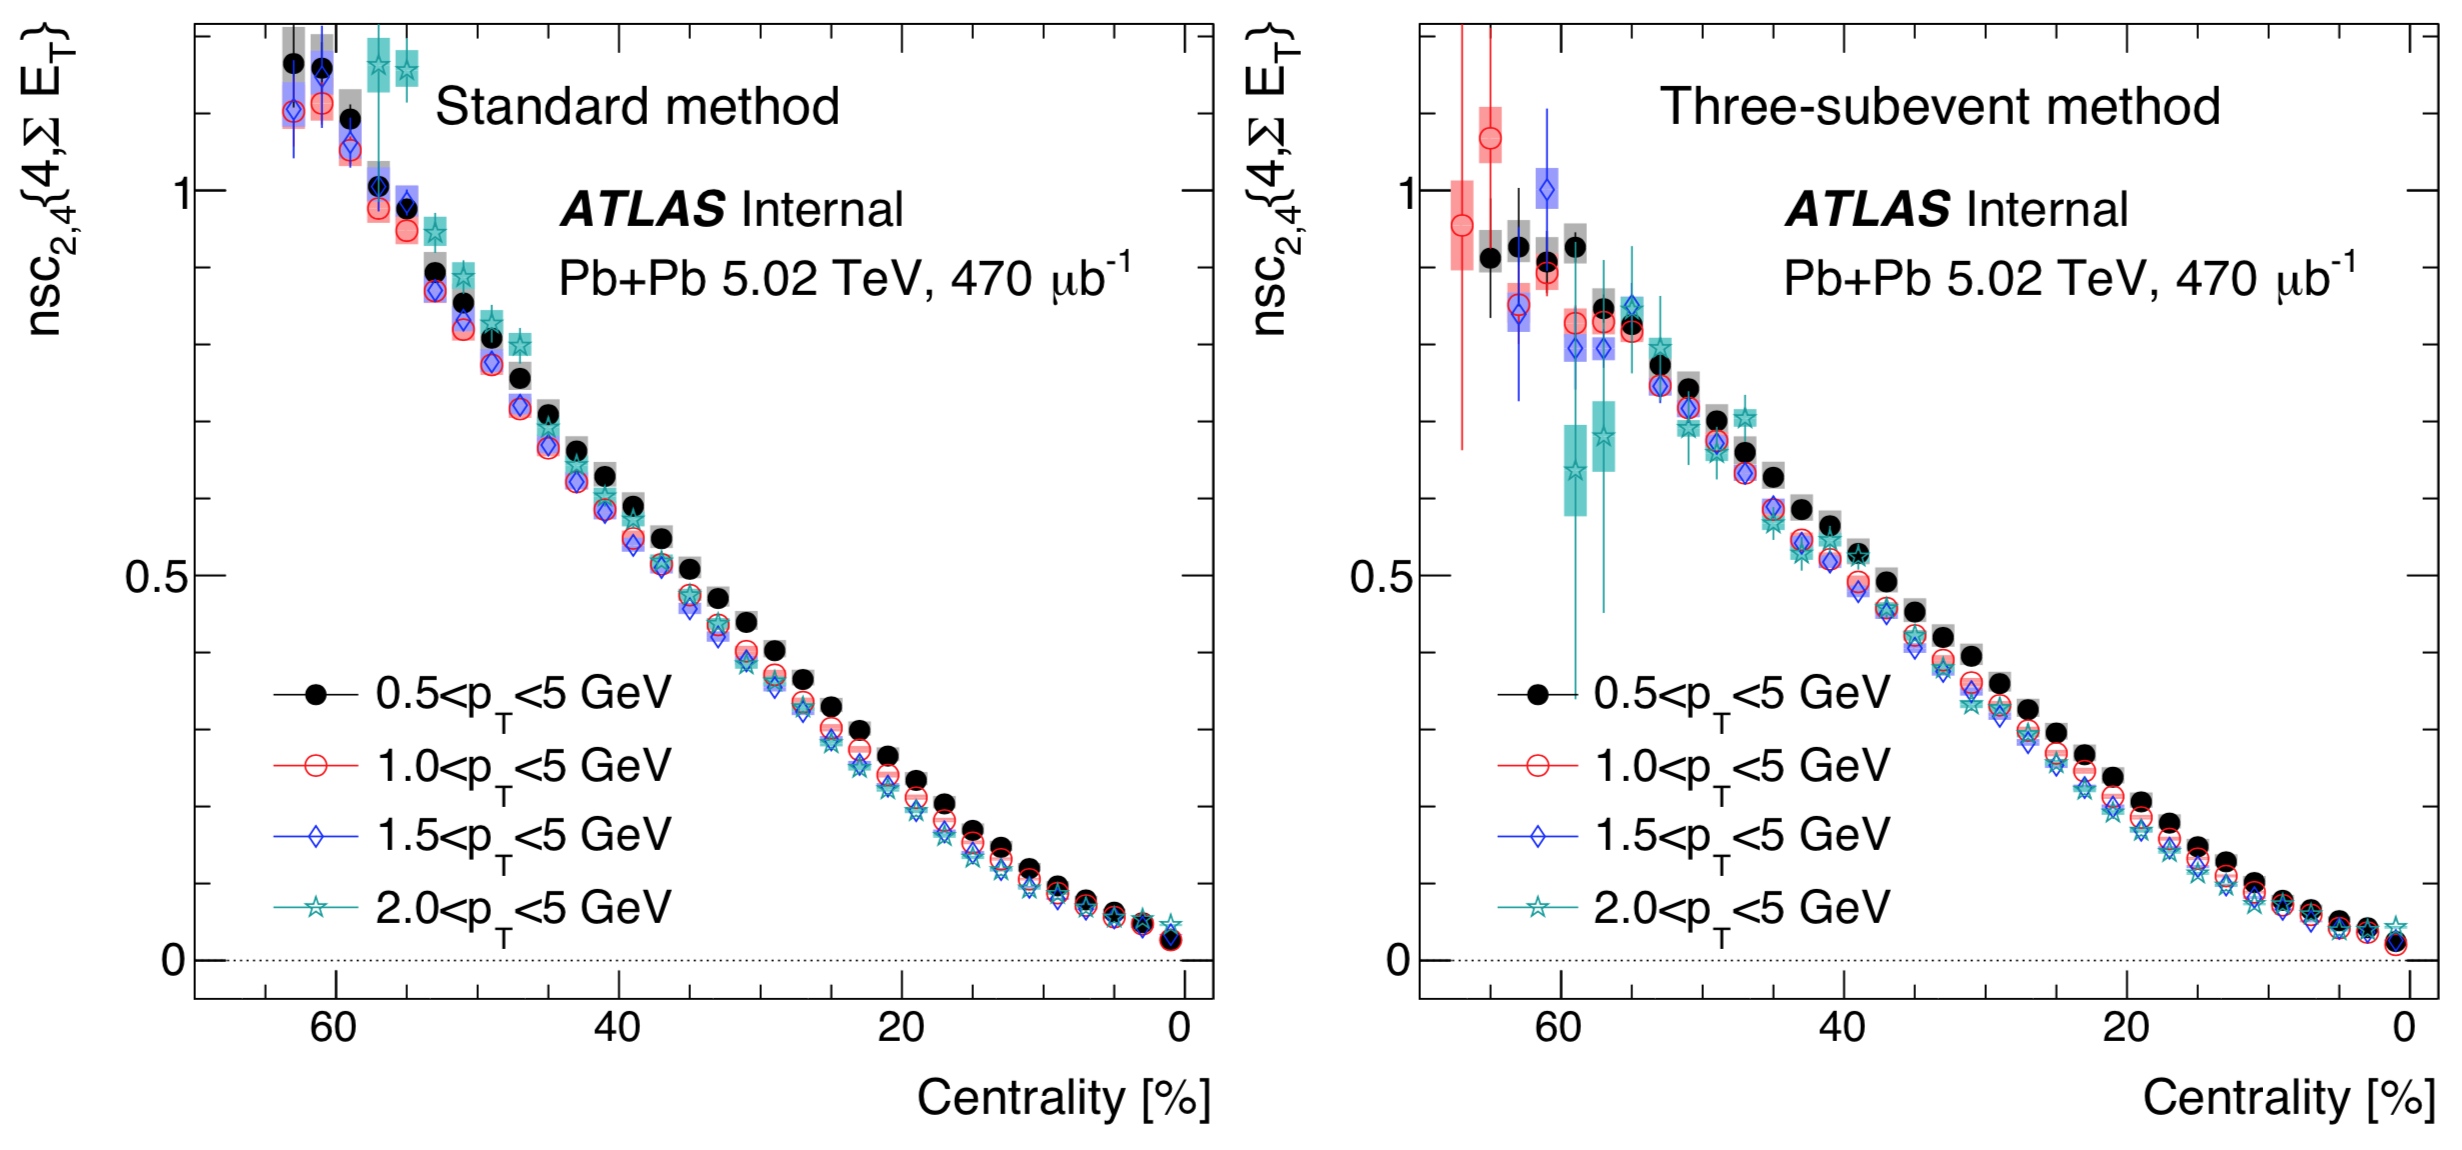
\includegraphics[width=.95\linewidth]{figs/chapter_centfluc/ATLAS_nsc24.png}
\caption{The centrality dependence of $nsc_{2,4}\{4\}$ calculated for charged particles in four $\pT$ ranges with the standard method (left) and three-subevent method (right). The error bars and shaded boxes represent the statistical and systematic uncertainties, respectively.}
\label{fig:centfluc_ATLAS_nsc24}
\end{figure}

Figure~\ref{fig:centfluc_ATLAS_nac2} shows the centrality dependence of $nac_2\{3\}$ in several $\pT$ ranges, which also probes the correlation between $v_2$ and $v_4$. The $nac_2\{3\}$ is positive over the entire centrality range. The correlation is weak in the central collisions, increases rapidly to around $20-30\%$ centrality range, and then increases slowly toward more peripheral collisions. The correlation patterns between different $\pT$ ranges are similar in central collisions, but are slightly weaker for higher $\pT$ particles in mid-central collisions. Comparing to results obtained from the three-subevent method, the results from the standard method are slightly larger in peripheral collisions, indicating that the non-flow may contribute for events beyond $60\%$ centrality. The similar $\pT$ and centrality dependences for $nsc_{2,4}\{4\}$ and $nac_2\{3\}$ are related to non-linear mode-mixing effects between $v_2$ and $v_4$~\cite{Giacalone:2016afq}.

\begin{figure}[H]
\centering
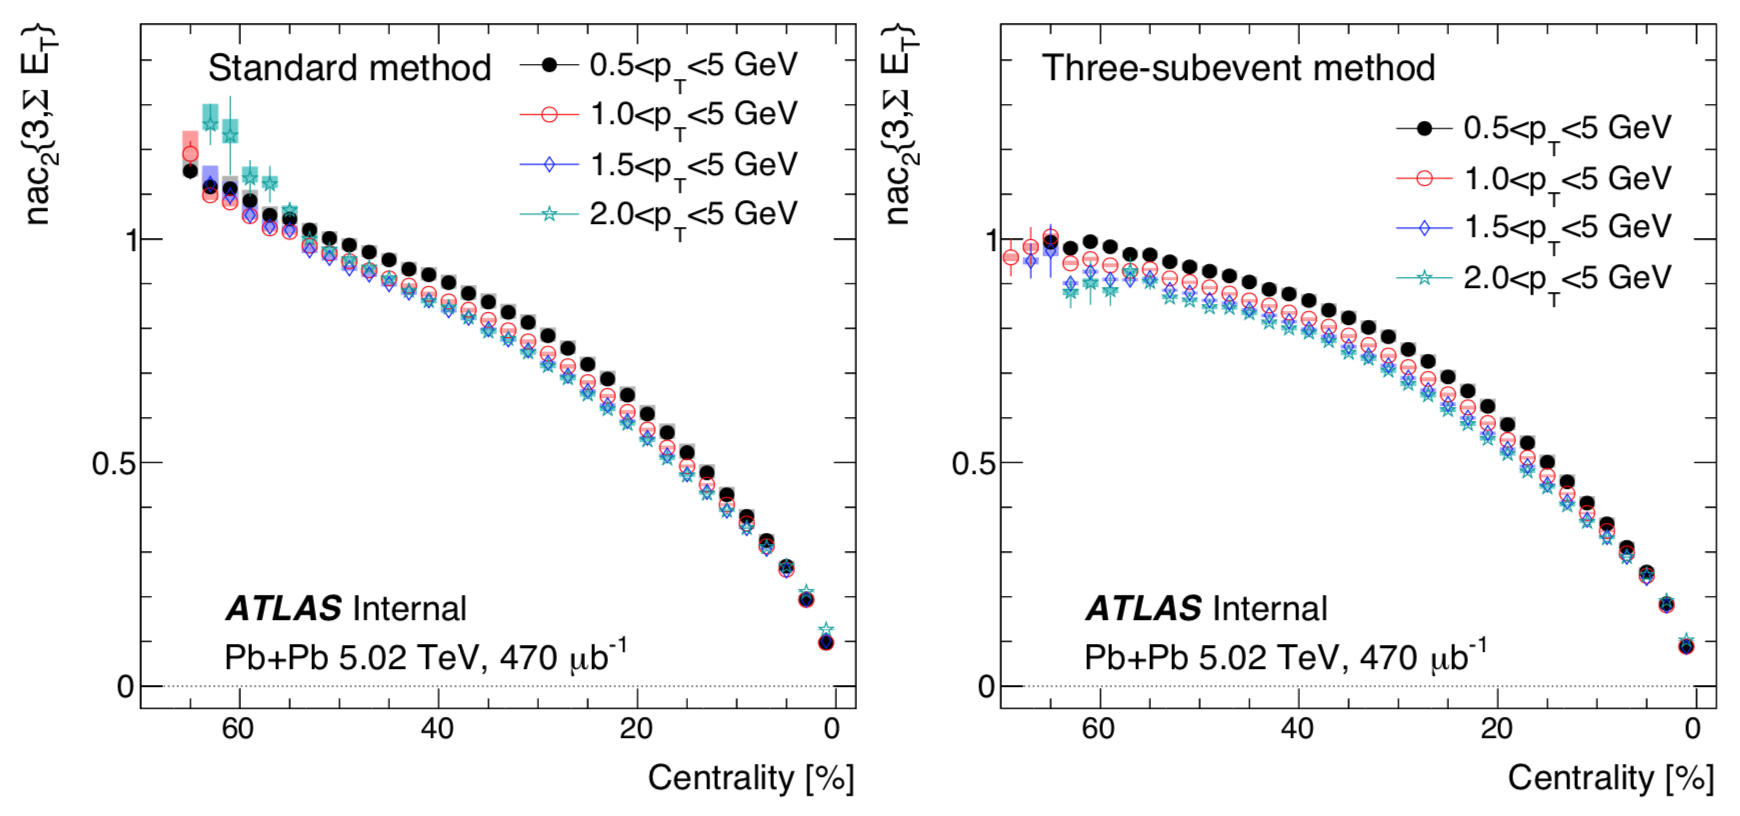
\includegraphics[width=.95\linewidth]{figs/chapter_centfluc/ATLAS_nac2.png}
\caption{The centrality dependence of $nac_{2}\{3\}$ calculated for charged particles in four $\pT$ ranges with the standard method (left) and three-subevent method (right). The error bars and shaded boxes represent the statistical and systematic uncertainties, respectively.}
\label{fig:centfluc_ATLAS_nac2}
\end{figure}



\paragraph{Dependence on reference event class and the role of centrality fluctuations}
\label{sec:dependence_on_reference_event_class_and_the_role_of_centrality_fluctuations}

The top panels of Figure~\ref{fig:centfluc_ATLAS_nc_4pc_cf1} show the $nc_n\{4, \Et\}$ as a function of $\lr{\Et}$. This figure contains the same information as the results shown in Figure~\ref{fig:centfluc_ATLAS_nc_4pc}, except for a change in the scale of the $x$-axis to show the central region with more details. The $nc_2\{4, \Et\}$ changes sign for $\lr{\Et} \ge (\Et)_\text{knee}$, where it first increases, reaches a maximum and then decreases to close to zero. The value of the maximum also increases with the $\pT$ of the particles. The $nc_3\{4, \Et\}$ is negative and approaches zero in ultra-central collisions, and only changes sign for the highest $\pT$ range used in this analysis. The $nc_4\{4, \Et\}$ changes from positive in peripheral collisions to negative in mid-central collisions, reaches a minimum and then turns back and approaches zero in the ultra-central collisions.

The bottom panels of Figure~\ref{fig:centfluc_ATLAS_nc_4pc_cf1} show the $nc_n\{4, \Nchrec\}$ as a function of $\lr{\Nchrec}$. The overall $\lr{\Nchrec}$ and $\pT$ dependence trends are similar to the top panels. However the maximum of $nc_2\{4, \Nchrec\}$ is more than factor of two larger, and $nc_3\{4, \Nchrec\}$ shows a clear sign change for the two highest $\pT$ ranges used in this analysis. Furthermore, the $nc_4\{4, \Nchrec\}$ shows a local maxima in ultra-central collisions, a feature absent for $nc_4\{4, \Et\}$.

If $\pmb{V}_n \propto \epsilon_n$ is valid, the shape of $p(v_n)$ should be the same as the shape of $p(\epsilon_n)$ and $nc_n\{4\}=nc_n\{4, \epsilon\}$~\cite{Giacalone:2017uqx, Zhou:2018fxx}. The $nc_n{4, \epsilon}$ can be estimated in a simple Glauber model framework using participating nucleons in the overlap region. As shown in Section~\ref{sec:flow_cumulants_for_pvn}, the $nc_n\{4, \epsilon\}$ is found to be always negative when the reference event class is defined based on the number of participating nucleons, $N_\text{part}$, or the impact parameter of the collisions~\cite{Alver:2008zza}. However, a positive $nc_n\{4, \epsilon\}$ is observed in ultra-central collisions when the reference event class is defined based on the final state particle multiplicity~\cite{Zhou:2018fxx, Agakishiev:2011eq}. Due to multiplicity smearing, events with the same final-state multiplicity can have different $N_\text{part}$, and therefore different $\epsilon_n$. The positive $nc_n\{4, \epsilon\}$ reflects the non-Gaussianity of $p(\epsilon_n)$ due to smearing in $N_\text{part}$ for events with the same final-state multiplicity. The larger values of $nc_n\{4, \Nchrec\}$ compared to $nc_n\{4, \Et\}$ in ultra-central collisions could be due to stronger multiplicity smearing for $nc_n\{4, \Nchrec\}$.

\begin{figure}[H]
\centering
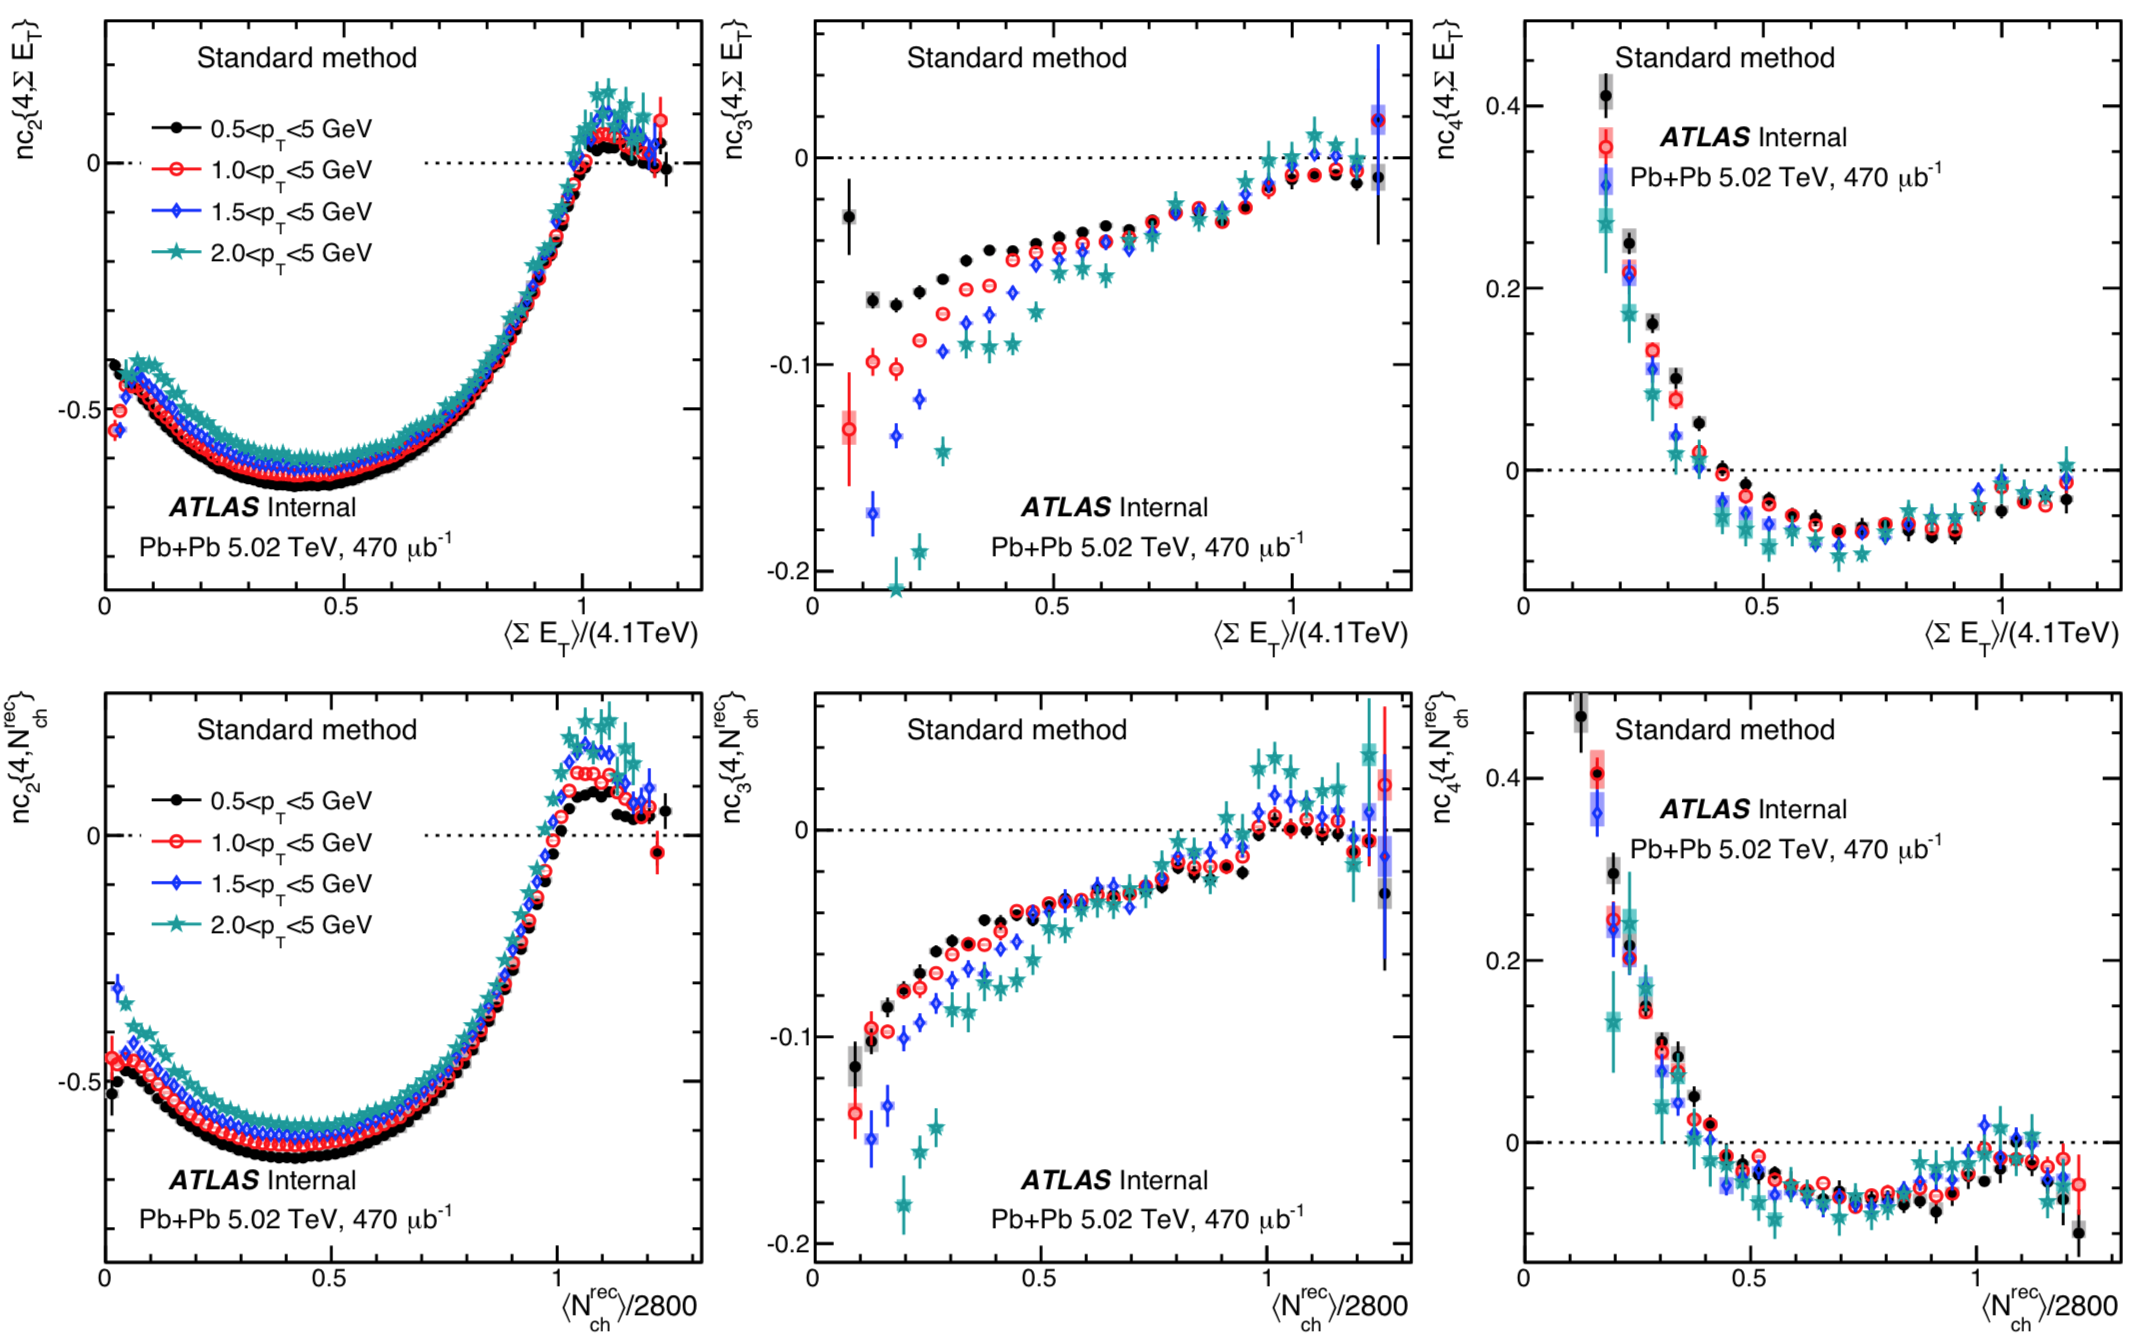
\includegraphics[width=.95\linewidth]{figs/chapter_centfluc/ATLAS_nc_4pc_cf1.png}
\caption{The normalized four-particle cumulants $nc_n\{4, \Et\}$ as a function of $\lr{\Et}$ (top row) and $nc_n\{4, \Nchrec\}$ as a function of $\lr{\Nchrec}$ (borrow row) for $n=2$ (left), $n=3$ (middle) and $n=4$ (right) for four $\pT$ ranges. The error bars and shaded boxes represent the statistical and systematic uncertainties, respectively.}
\label{fig:centfluc_ATLAS_nc_4pc_cf1}
\end{figure}

Figure~\ref{fig:centfluc_ATLAS_nc_4pc_cf2} compares the $nc_n\{4, \Et\}$ and $nc_n\{4, \Nchrec\}$ as a function of $\lr{\Et}$ obtained for $1.5<\pT<5.0$ GeV. In both cases, the normalized cumulants for $v_2$ and $v_3$ show significant differences between the two reference event classes, while that for $v_4$ are more similar. The values of $nc_n\{4, \Nchrec\}$ for $n=2$ and $n=3$ are significantly than those for $nc_n\{4, \Et\}$ over a broad centrality range, not only limited to the ultra-central collisions. This implies that the influence of centrality fluctuations are potentially important even in mid-central collisions.

\begin{figure}[H]
\centering
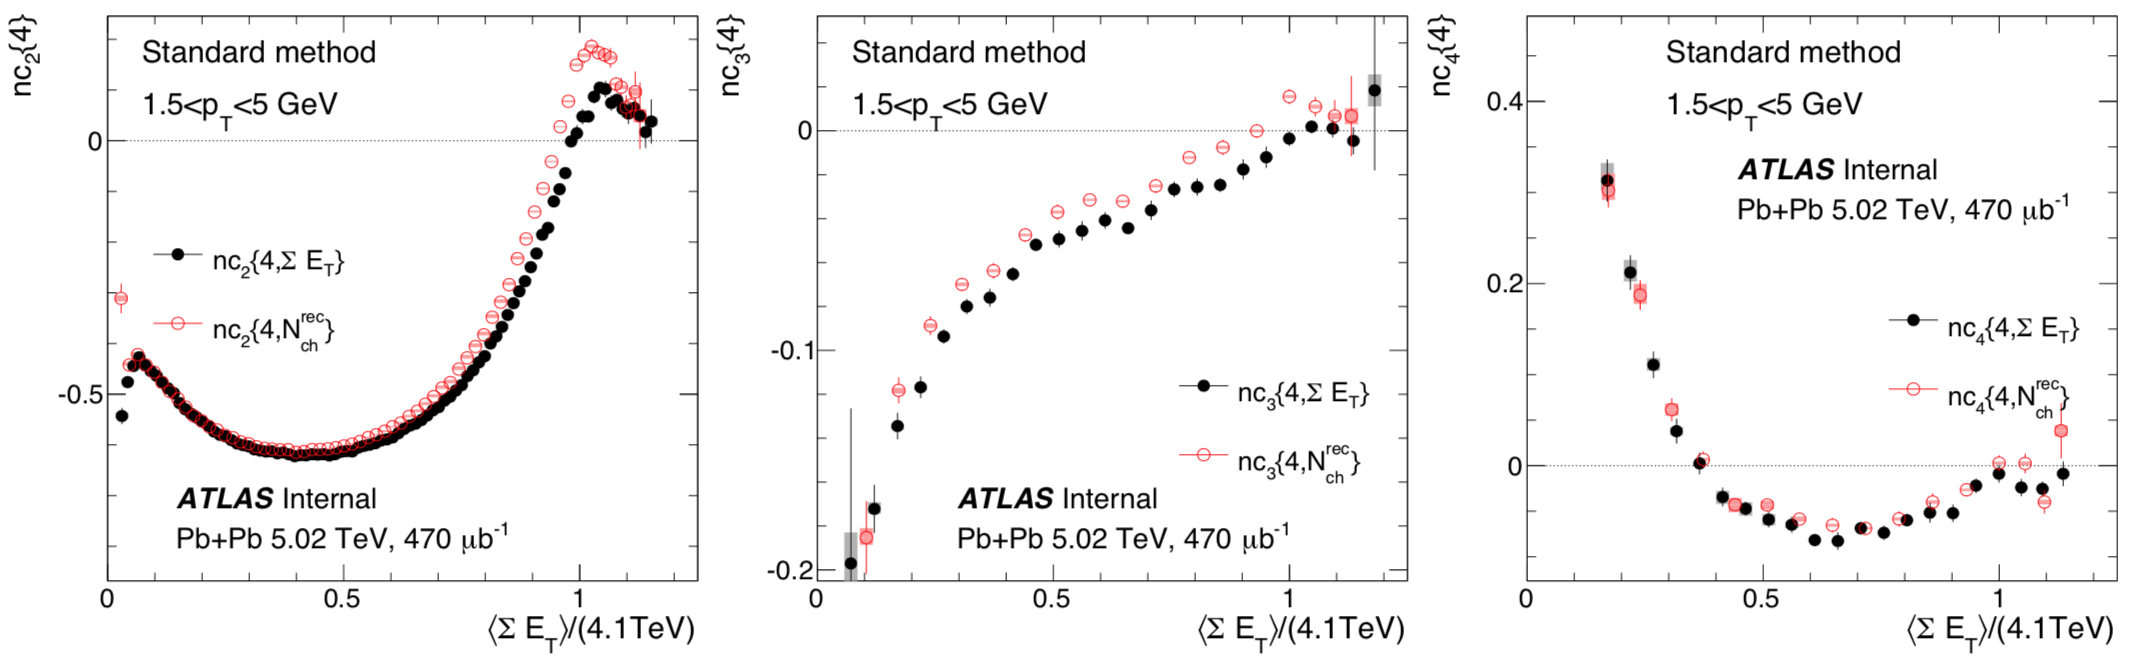
\includegraphics[width=.95\linewidth]{figs/chapter_centfluc/ATLAS_nc_4pc_cf2.png}
\caption{The comparison of normalized four-particle cumulants $nc_n\{4, \Et\}$ and $nc_n\{4, \Nchrec\}$ as a function of $\lr{\Et}$ for $n=2$ (left), $n=3$ (middle) and $n=4$ (right) for charged particles $1.5<\pT<5.0$ GeV. The error bars and shaded boxes represent the statistical and systematic uncertainties, respectively.}
\label{fig:centfluc_ATLAS_nc_4pc_cf2}
\end{figure}

The left two panels of Figure~\ref{fig:centfluc_ATLAS_nc_6pc_cf} show the six-particle normalized cumulants for $v_2$ obtained using the two reference event classes, $nc_2\{6, \Et\}$ and $nc_2\{6, \Nchrec\}$, respectively. The $nc_2\{6\}$ values are positive in most of the centrality range. But decrease to zero at around $\lr{\Et} = (\Et)_\text{knee}$ or $\lr{\Nchrec} = (\Nchrec)_\text{knee}$ and stay close to zero above that. The right panel of Figure~\ref{fig:centfluc_ATLAS_nc_6pc_cf} compares $nc_2\{6, \Et\}$ and $nc_2\{6, \Nchrec\}$ as a function of $\lr{\Et}$. The values of $nc_2\{6, \Nchrec\}$ are found to be smaller than those for $nc_2\{6, \Et\}$ in central and mid-central collisions, suggesting that the centrality  fluctuations influence the multi-particle cumulants of $p(v_2)$ over a broad centrality range.

\begin{figure}[H]
\centering
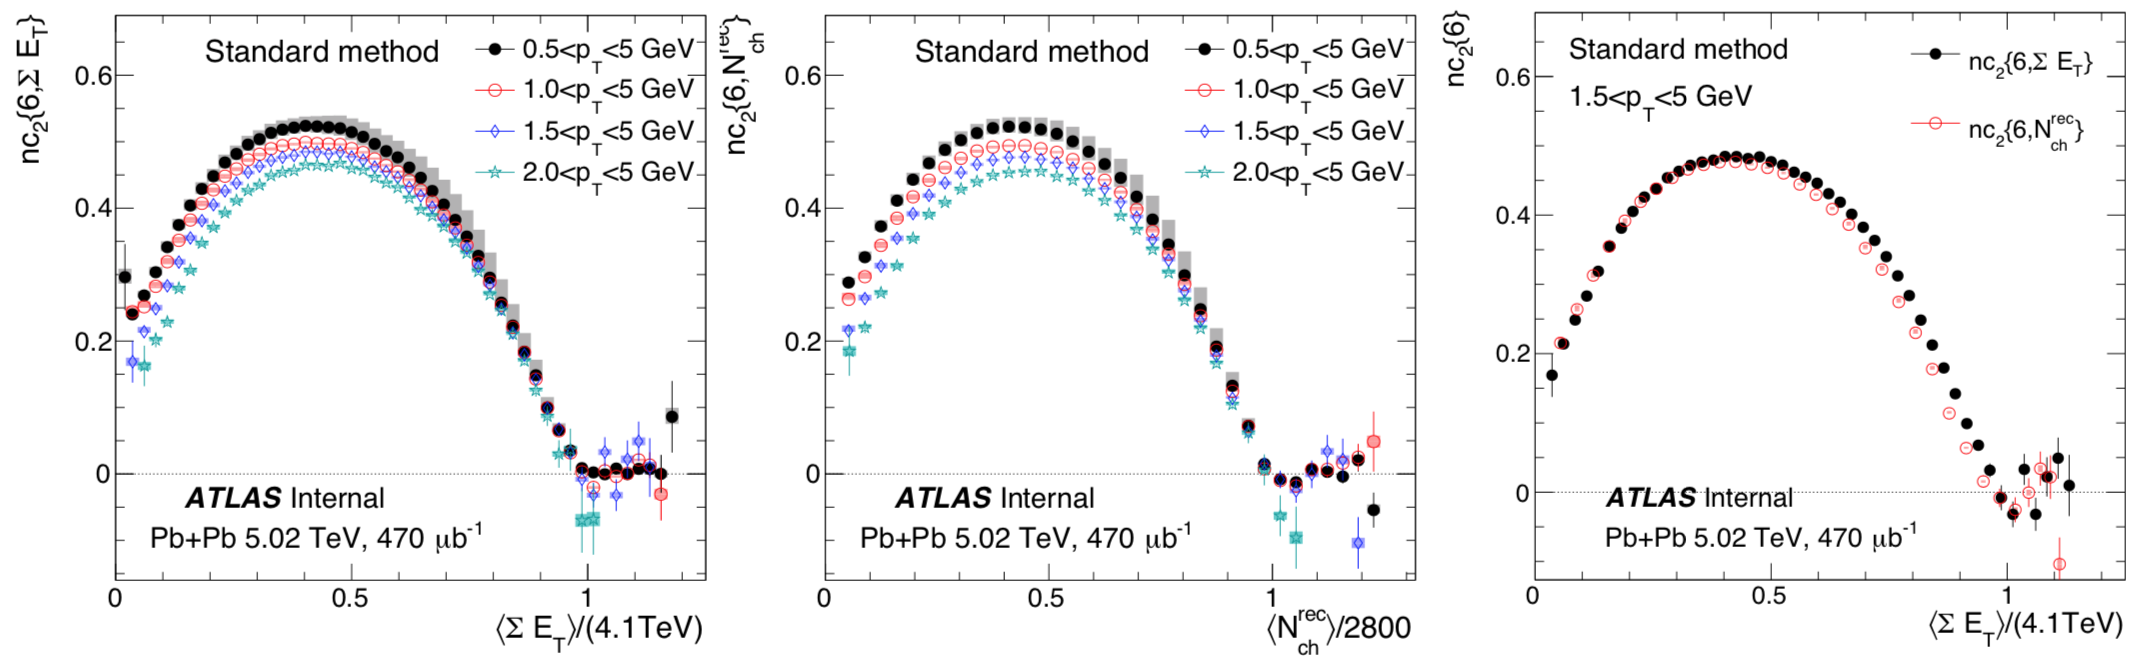
\includegraphics[width=.95\linewidth]{figs/chapter_centfluc/ATLAS_nc_6pc_cf.png}
\caption{The normalized six-particle cumulants $nc_2\{6, \Et\}$ as a function of $\lr{\Et}$ (left) and $nc_2\{6, \Nchrec\}$ as a function of $\lr{\Nchrec}$ (middle) in four $\pT$ ranges. The $nc_2\{6, \Et\}$ and $nc_2\{6, \Nchrec\}$ results for $1.5<\pT<5.0$ GeV are also compared directly as a function of $\lr{\Et}$ (right). The error bars and shaded boxes represent the statistical and systematic uncertainties, respectively.}
\label{fig:centfluc_ATLAS_nc_6pc_cf}
\end{figure}

The left panel of Figure~\ref{fig:centfluc_ATLAS_v2_64pc_ratio_cf} shows the cumulant ratio $v_2\{6\} / v_2\{4\}$, obtained for event class based on $\Et$. This panel contains the same information as those shown in Figure~\ref{fig:centfluc_ATLAS_v2_64pc_ratio}, except for a change in the scale of the $x$-axis to show the central region in more details. The data show significant differences among the four $\pT$ ranges. The values of $v_2\{6\} / v_2\{4\}$ is larger for higher $\pT$, even exceeds one in ultra-central collisions. This behavior is expected, as the $c_2\{4\}$ and therefore $v_2\{4\}$ changes sign in ultra-central collisions. The right panel of Figure~\ref{fig:centfluc_ATLAS_v2_64pc_ratio_cf} shows $v_2\{6\} / v_2\{4\}$ obtained for event class based on $\Nchrec$, but then mapped on to $\lr{\Et}$. The differences of the results between various $\pT$ ranges are larger for majority of the centrality range, which again implies that the centrality fluctuations influence the ratios between multi-particle cumulants over a broad centrality range.

\begin{figure}[H]
\centering
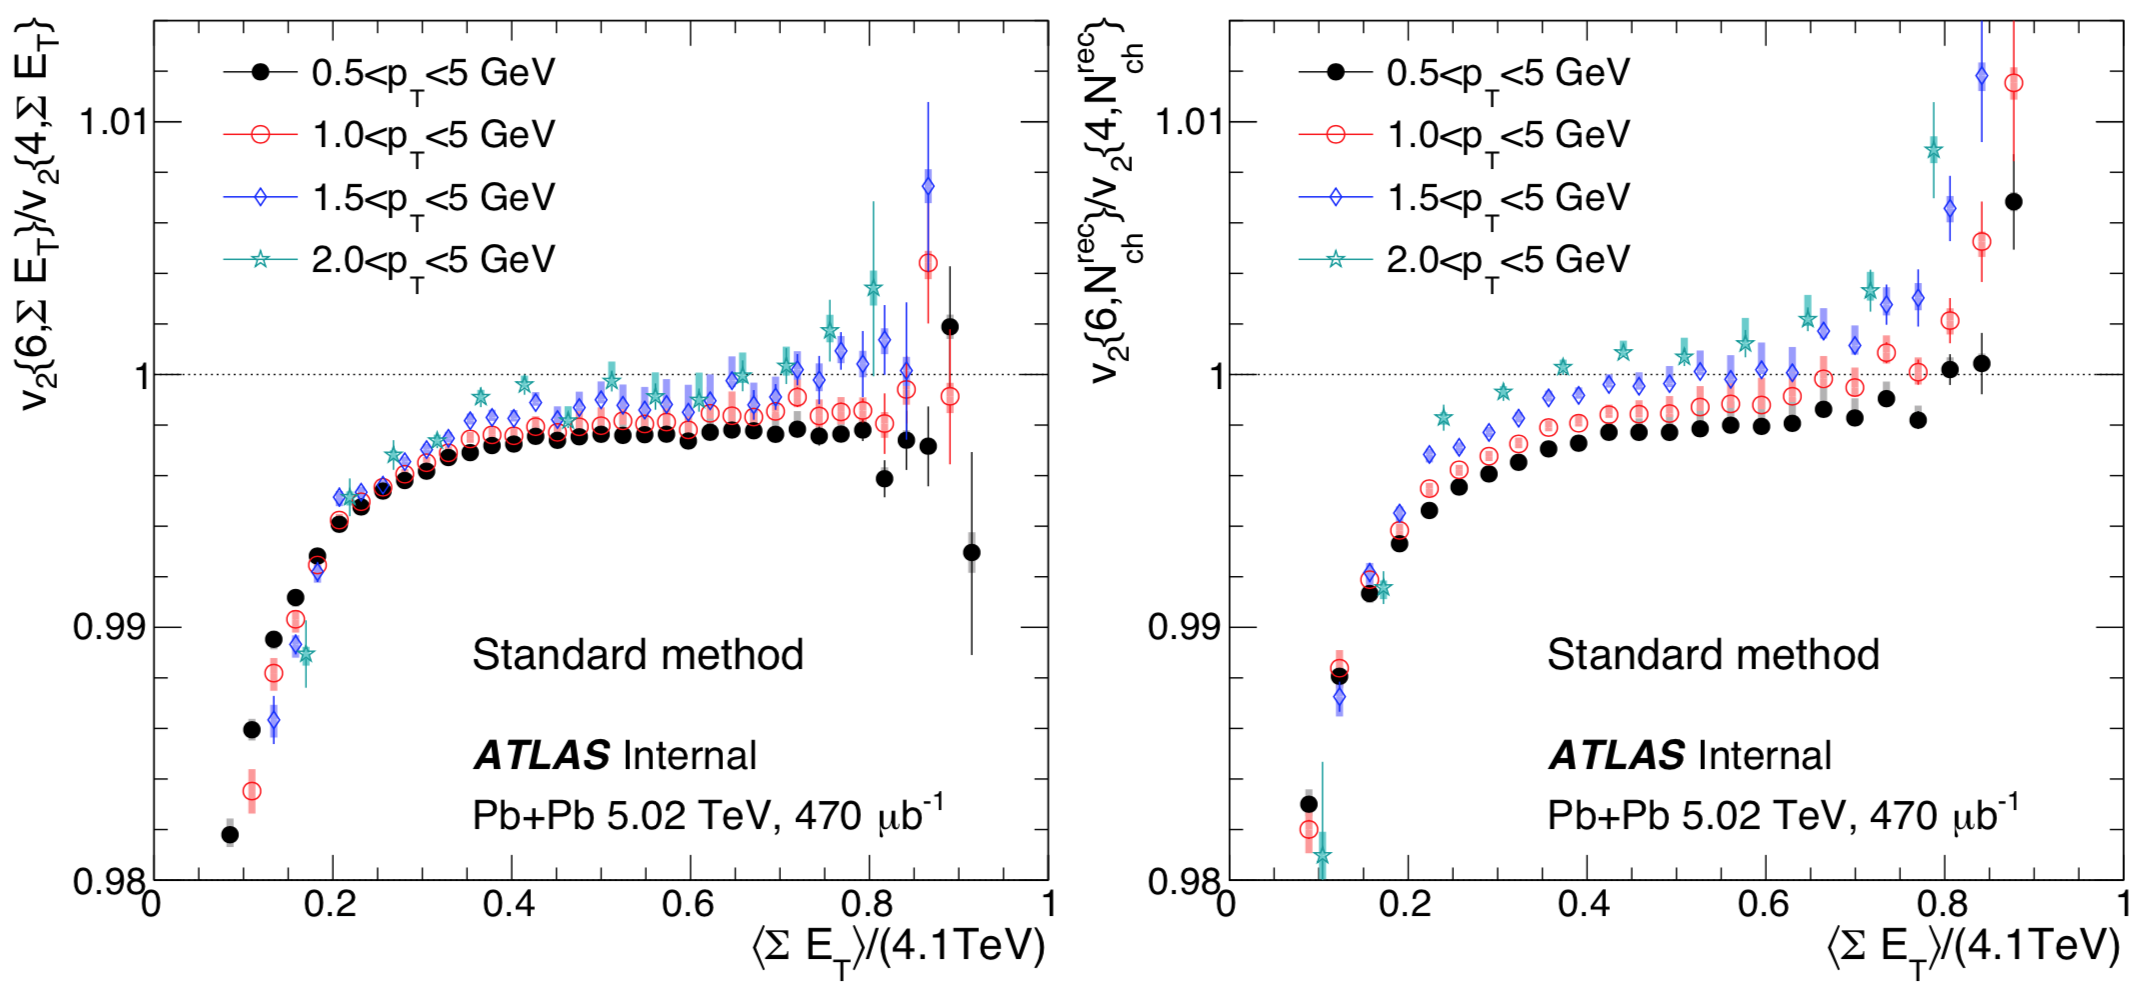
\includegraphics[width=.95\linewidth]{figs/chapter_centfluc/ATLAS_v2_64pc_ratio_cf.png}
\caption{The $\lr{\Et}$ dependence of cumulant ratio $v_2\{6, \Et\} / v_2\{4, \Et\}$ (left) and $v_2\{6, \Nchrec\} / v_2\{4, \Nchrec\}$ (right) for charged particles in four $\pT$ ranges. The error bars and shaded boxes represent the statistical and systematic uncertainties, respectively.}
\label{fig:centfluc_ATLAS_v2_64pc_ratio_cf}
\end{figure}

The sensitivity on the choice of reference event class is also studied for symmetric cumulants $nc_{2,3}\{4\}$, $nc_{2,4}\{4\}$ and asymmetric cumulant $nac_2\{3\}$. The results obtained with event class based on $\Et$ are shown in the top row of Figure~\ref{fig:centfluc_ATLAS_others_cf1} as a function of $\lr{\Et}$. The $nsc_{2,3}\{4, \Et\}$ values change sign and become positive in ultra-central collisions, and they are larger at higher $\pT$. At the largest $\lr{\Et}$ values, the $nc_{2,4}\{4, \Et\}$ reaches zero or even becomes slightly negative, which $nac_2\{3, \Et\}$ reaches around 0.05. The bottom three panels of Figure~\ref{fig:centfluc_ATLAS_others_cf1} show the similar results but obtained with event class based on $\Nchrec$. The positive $nsc_{2,3}\{4, \Nchrec\}$ values in the ultra-central region are larger than those for $nsc_{2,3}\{4, \Et\}$. The trends of the other two cumulants are similar to those obtained with event class based on $\Et$.

\begin{figure}[H]
\centering
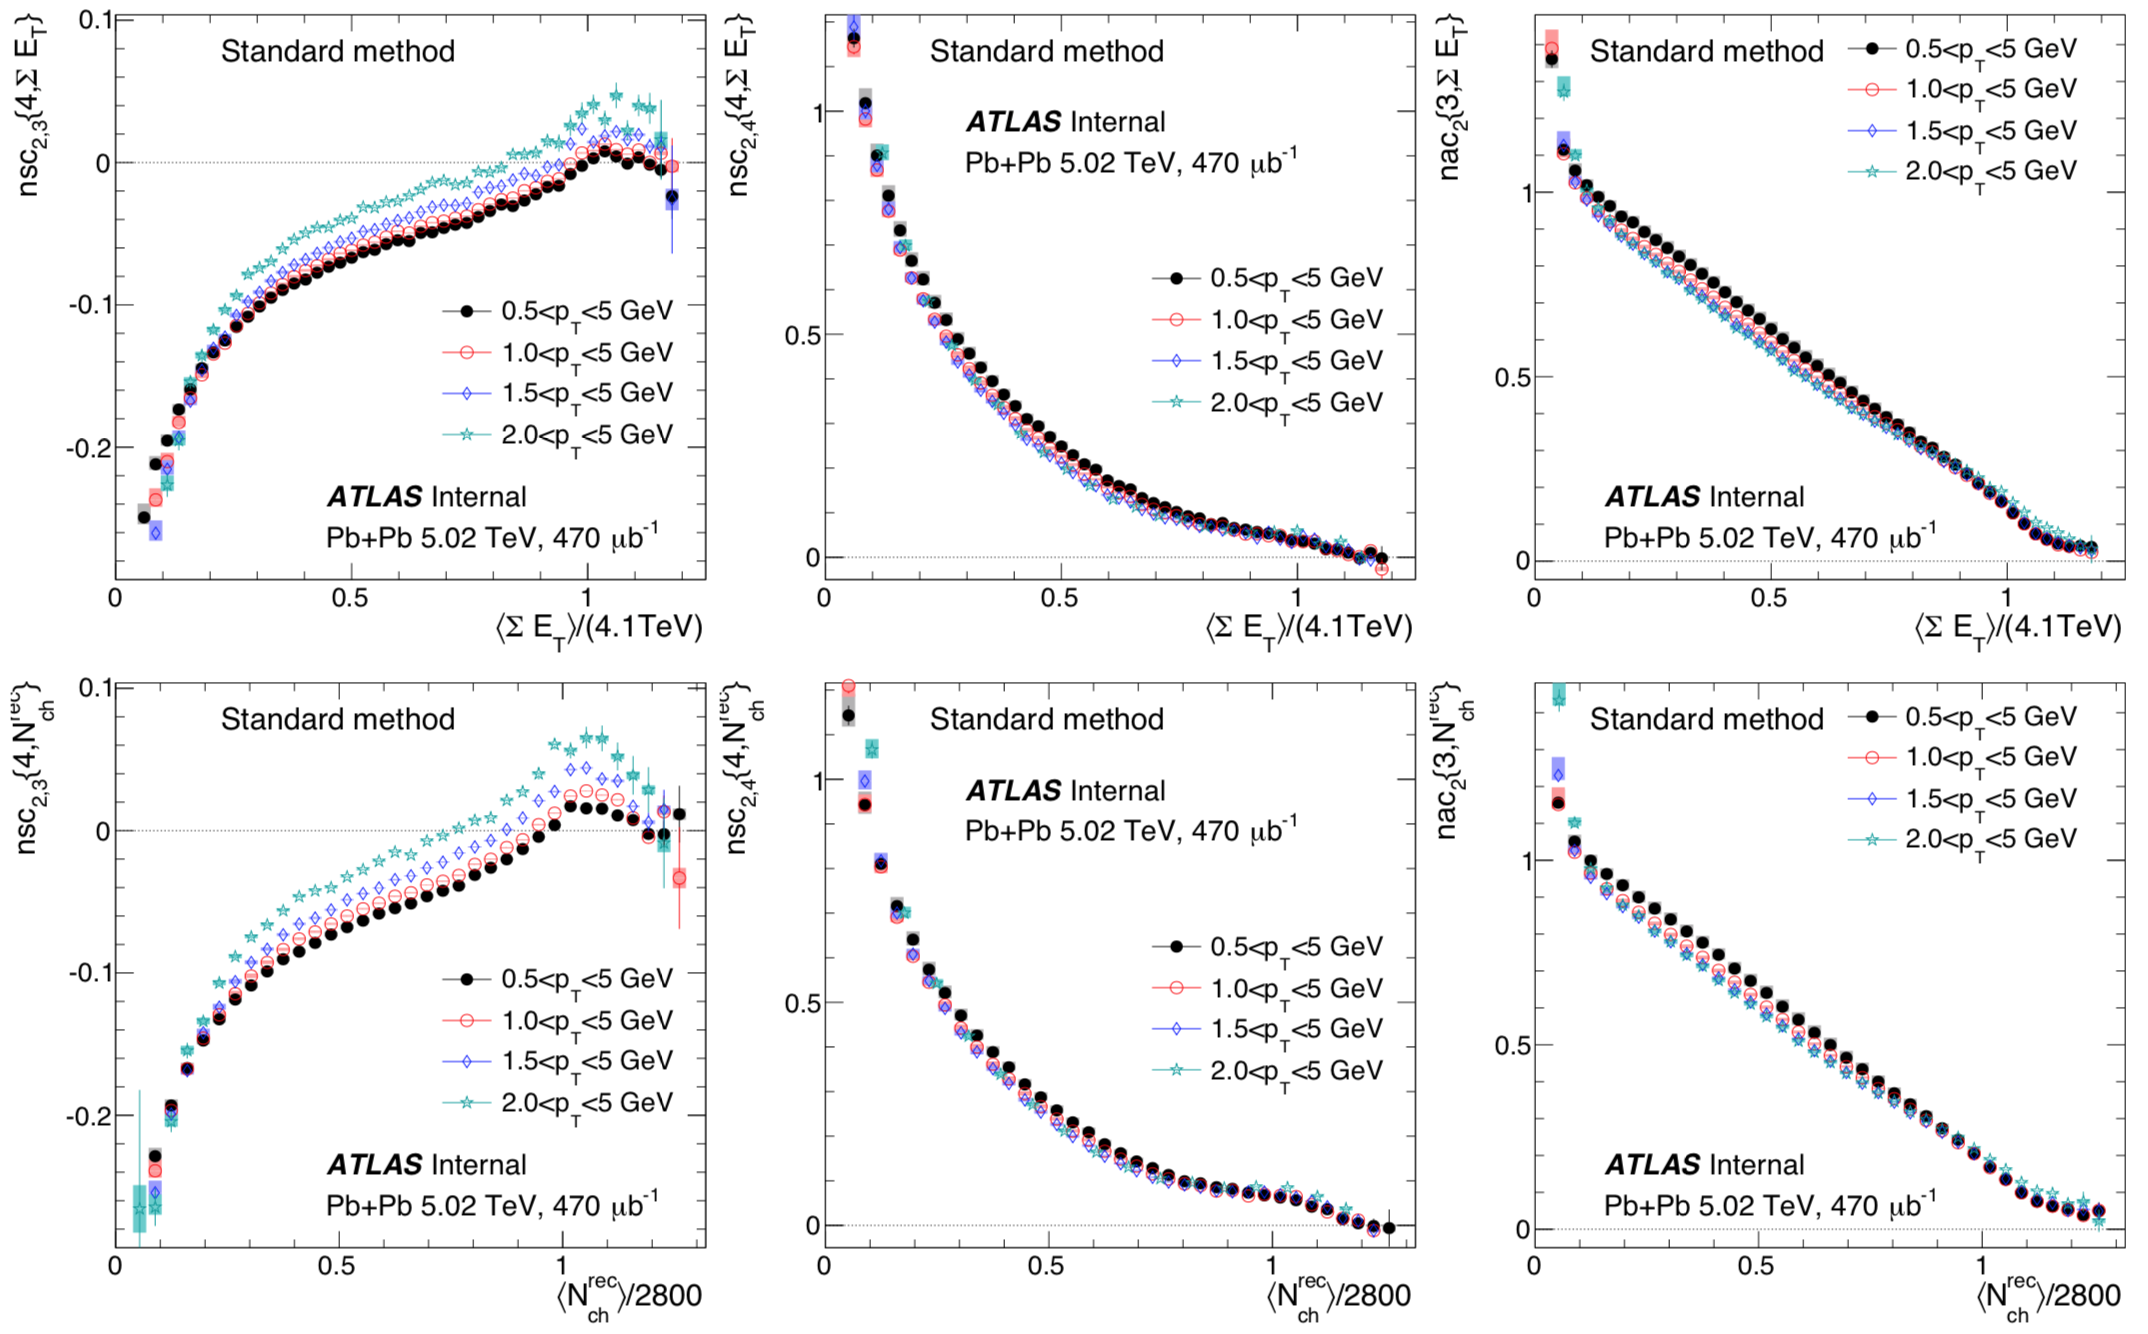
\includegraphics[width=.95\linewidth]{figs/chapter_centfluc/ATLAS_others_cf1.png}
\caption{The top row shows the $\lr{\Et}$ dependence of normalized cumulants $nsc_{2,3}\{4, \Et\}$ (left), $nsc_{2,4}\{4, \Et\}$ (middle) and $nac_2\{3, \Et\}$ (right) for four $\pT$ ranges. The top row shows the $\lr{\Nchrec}$ dependence of normalized cumulants $nsc_{2,3}\{4, \Nchrec\}$ (left), $nsc_{2,4}\{4, \Nchrec\}$ (middle) and $nac_2\{3, \Nchrec\}$ (right) for four $\pT$ ranges. The error bars and shaded boxes represent the statistical and systematic uncertainties, respectively.}
\label{fig:centfluc_ATLAS_others_cf1}
\end{figure}

The direct comparison of $nsc_{2,3}\{4\}$, $nsc_{2,4}\{4\}$ and $nac_2\{3\}$ obtained with the two reference event classes are shown in Figure~\ref{fig:centfluc_ATLAS_others_cf2} for particles with $1.5<\pT<5.0$ GeV as a function of $\lr{\Et}$. The values of $nsc_{2,3}\{4, \Nchrec\}$ are larger than those for $nsc_{2,3}\{4. \Et\}$ in central and mid-central collisions. On the other hand, the values of the other two cumulants are similar between the two reference event class.

\begin{figure}[H]
\centering
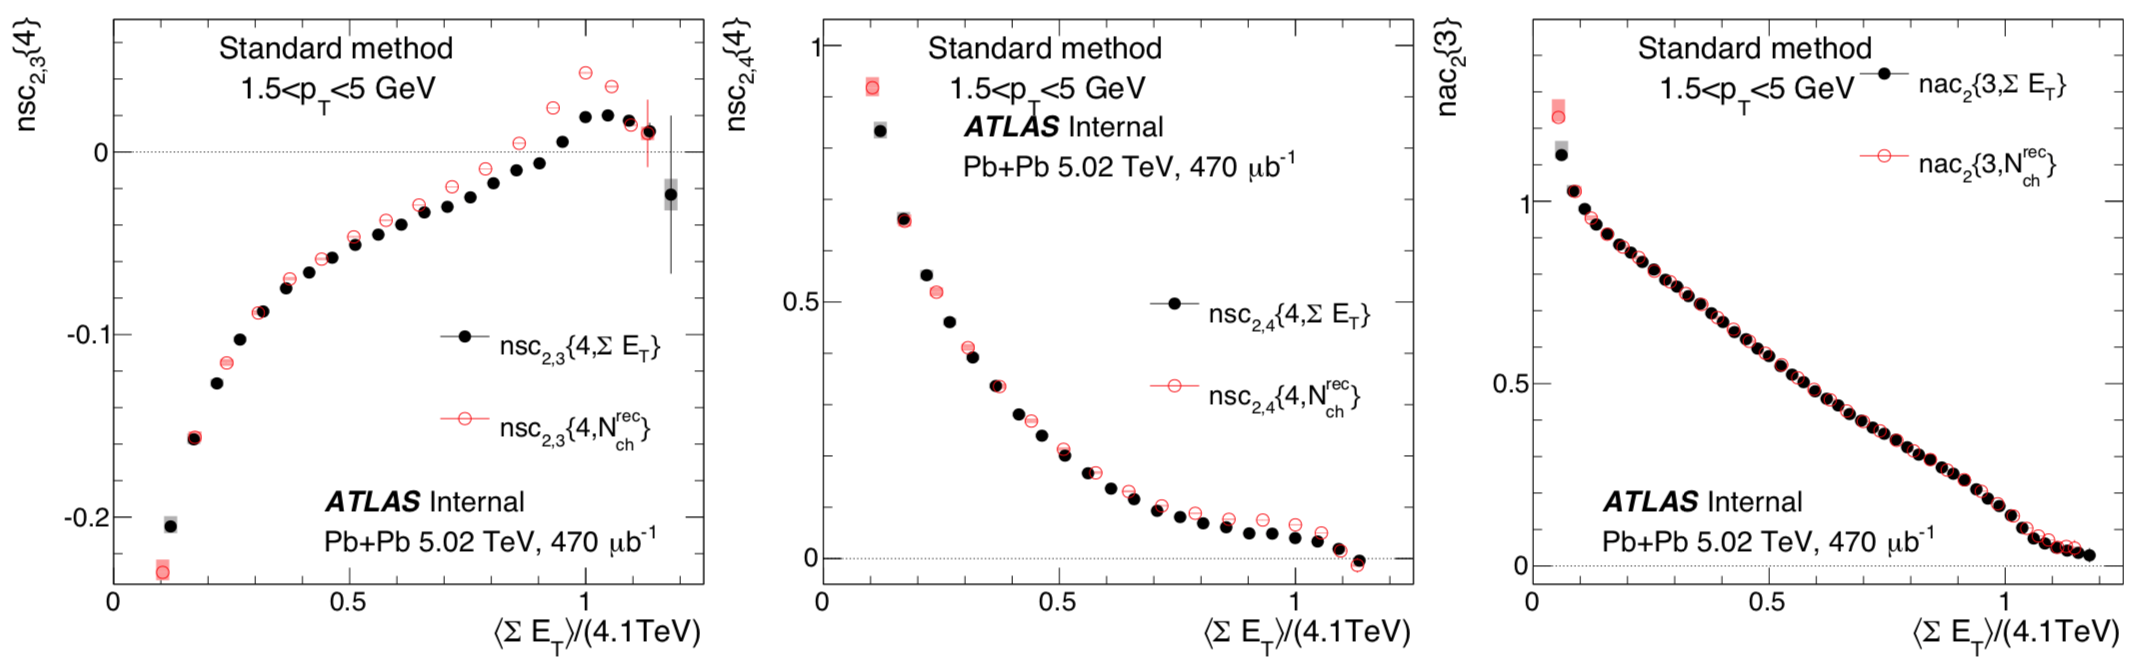
\includegraphics[width=.95\linewidth]{figs/chapter_centfluc/ATLAS_others_cf2.png}
\caption{Comparison of $nsc_{2,3}\{4, \Et\}$ and $nsc_{2,3}\{4, \Nchrec\}$ (left), $nsc_{2,4}\{4, \Et\}$ and $nsc_{2,4}\{4, \Nchrec\}$ (middle), and $nac_{2}\{3, \Et\}$ and $nac_{2}\{3, \Nchrec\}$ (right) as a function of $\lr{\Et}$. The error bars and shaded boxes represent the statistical and systematic uncertainties, respectively.}
\label{fig:centfluc_ATLAS_others_cf2}
\end{figure}



\subsection{Summary and discussion}

\subsubsection{Flow fluctuation}

Using Pb+Pb collisions at $\sqrt{s_\text{NN}} = 5.02$ TeV with the ATLAS detector, we studied the event-by-event fluctuations of one harmonic $p(v_n)$ or two different harmonics $p(v_n, v_m)$. The $p(v_n)$ is studied via $2k$-particle cumulants $c_n\{2k\}$ and normalized cumulants $nc_n\{2k\}$, which provide estimate of the flow coefficients $v_n\{2k\}$ and cumulant ratios $v_n\{4\} / v_n\{2\}$ and $v_n\{6\} / v_n\{4\}$. The $p(v_n, v_m)$ is studied using the so-called normalized symmetric cumulant $nsc_{n,m}\{4\}$ and asymmetric cumulant $nac_2\{3\}$. These normalized cumulants are directly sensitive to the fluctuations of collision geometry in the initial state.

Our studies provide a first observation of a negative $c_1\{4\}$ and therefore a positive $v_1\{4\}$, which sheds light on the nature of the dipolar eccentricity fluctuation in the initial-state geometry. The values of $c_4\{4\}$ are found to be negative in central collisions but change sign around $20-25\%$ centrality and increase quickly for more peripheral collisions. This behavior is consistent with a nonlinear contribution to $v_4$ that is proportional to $v_2^2$. This non-linear contribution increases for more peripheral collisions and has a positive contribution to $c_4\{4\}$. Over most of the centrality range, the $c_2\{4\}$ and $c_3\{4\}$ are found to be negative , but change sign towards most central collisions, suggesting that the $p(v_2)$ and $p(v_3)$ distributions deviate significantly from a Gaussian shape. The cumulant ratios $v_2\{4\} / v_2\{2\}$, $v_3\{4\} / v_3\{2\}$, $v_4\{4\} / v_4\{2\}$ and $v_2\{6\} / v_2\{4\}$ exhibit small but significant $\pT$ dependence, suggesting flow fluctuations may also arise directly in the momentum space through the initial state correlations or final state interactions.

Our study also present a detailed measurement of four-particle symmetric cumulants $nsc_{2,3}\{4\}$, $nsc_{2,4}\{4\}$ and three-particle asymmetric cumulant $nac_2\{3\}$. The symmetric cumulants probe the correlation between the magnitudes of two flow harmonics, while asymmetric cumulant is sensitive to correlation involving both the magnitude and phase of flow. Over most of the centrality range, the $nsc_{2,3}\{4\}$ is found to be negative, reflecting an anti-correlation between $v_2$ and $v_3$. The $nsc_{2,4}\{4\}$ and $nac_2\{3\}$ are found to be positive, and their dependence on centrality are consistent with non-linear mode-mixing effects between $v_2$ and $v_4$.

\subsubsection{Centrality fluctuation}

In heavy-ion collisions, due to fluctuations in the particle production process, the centrality or the volume of the fireball for events selected to have the same final-state particle multiplicity fluctuates from event to event. The so-called centrality fluctuations lead to significant uncertainties in interpreting centrality dependence of experimental observables.

With an independent source model framework, which simulates the particle multiplicity as a superposition of particles from $N_\text{s}$ uncorrelated sources in each event, we investigate the effects of centrality fluctuations on flow fluctuations. A Glauber model is used to simulate the transverse distribution of sources in each event and to calculate the eccentricity $\epsilon_n$. Following the standard experimental centrality selection procedure, the centrality fluctuations are imposed by selecting events with fixed $N$, which contribute to event-by-event fluctuations of eccentricities. The main goal of our model studies is to propose a set of cumulant observables related to these distributions and study their sensitivities to centrality fluctuations. To be specific, we studied the influence of the fluctuation of sources on the eccentricities $\epsilon_n$, which characterizes the shape of the collision zone and drives the final-state harmonic flow $v_n$. We found that the centrality fluctuations for a given centrality selection criteria influence significantly $p(\epsilon_n)$ and $p(\epsilon_n, \epsilon_m)$. This is especially true in central collisions, where eccentricity fluctuations are very sensitive to any non-Gaussian introduced by centrality fluctuations. Indeed, we found that the four-, six- and eight-particle cumulants for $\epsilon_2$ and $\epsilon_3$ exhibit rather complex sign-change patterns in central collisions, indicative of significant non-Gaussianity in $p(\epsilon_n)$. Similar sign-change patterns are also observed for four-particle symmetric cumulants between $\epsilon_2$ and $\epsilon_3$, and between $\epsilon_2$ and $\epsilon_4$, consistent with significant non-Gaussianity of $p(\epsilon_2, \epsilon_3)$ and $p(\epsilon_2, \epsilon_4)$ in central collisions. We found these eccentricity cumulants are sensitive to the underlying $p(N_\text{s})$; they are also sensitive to the $\hat{\sigma}$ of $p(n)$ but not its functional form.

In experimental measurements, the cumulants are always calculated for events with similar activity. However, for a given activity measure, fluctuations in the particle production process lead to irreducible centrality fluctuations. To study the influence of centrality of centrality fluctuations, cumulant observables are calculated for the two reference event classes with different centrality resolution: the total transverse energy in $3.2<|\eta|<4.9$, and number of reconstructed charged particles in $|\eta|<2.5$ with $0.5<\pT<5.0$ GeV. In ultra-central collisions, several cumulants $nc_2\{4\}$, $nc_3\{4\}$ and $nsc_{2,3}\{4\}$, are observed to change sign, indicating a significant influence of centrality fluctuations on the multi-particle cumulants of $p(v_2)$, $p(v_3)$ and $p(v_2, v_3)$. The sign change patterns are more pronounced for event class based on $\lr{\Nchrec}$, consistent with a larger centrality fluctuations. The differences between the two event classes are found to persist, with decreasing magnitude, to mid-central collisions, which may suggest that the centrality fluctuations influence the flow fluctuations over a broad centrality range. The sign change patterns are found to be more pronounced at higher $\pT$, which may indicate that the flow fluctuations have significant $\pT$ dependence. Such $\pT$ dependence can not be explained by considering only fluctuations in the initial geometry.

Our model and ATLAS data results provide comprehensive information on the nature of flow fluctuations and the contributions from both the initial state and the final state. They also shed light on the influence of centrality fluctuations on flow fluctuations, especially in the ultra-central collisions, which can help to clarify the meaning of centrality and provide insights on the sources for particle production in heavy-ion collisions.



\subsection{Outlook}

\subsubsection{Smaller collision system: Xe+Xe}
\label{sec:novel_collision_systems_xexe}

In October 2017, the ATLAS experiment recorded collisions of xenon nuclei for the first time. While massive compared to a proton, xenon nuclei are smaller than the lead ions typically collided in the LHC (129 nucleons compared to 208 nucleons and a nuclear radii of 5.4 fm compared to 6.6 fm). The xenon-xenon collision data, combined with previous results from the analysis of lead-lead collisions, proved the first opportunity to examine heavy ion collisions in a system that is distinctly smaller in size. This allows physicists to study in detail the role of the collision geometry for observables often associated with the QGP.

The left panel of Figure~\ref{fig:centfluc_ATLAS_Xe_cn} shows the centrality dependence of 4- and 6-particle flow cumulants $v_n\{2k\}$, using particles in $0.5<\pT<5.0$ GeV. For $v_2$, different orders of cumulants have similar centrality dependence: largest in mid-central and decreasing towards both central and peripheral. The ordering $v_2\{\text{2PC}\} > v_2\{4\} \approx v_2\{6\}$ is observed, which indicates that $v_2$ fluctuations are close to Gaussian. For $v_3$ only the 4-particle cumulant $v_3\{4\}$ is measured, and $v_3\{6\}$ is not shown since its statistical uncertainties are very large. The centrality dependence of $v_3$ is similar to $v_2$, and $v_3\{\text{2PC}\}$ is two times larger than $v_3\{4\}$, indicating strong $v_3$ flow fluctuations.

To quantify the type and strength of flow fluctuations, cumulant ratios $v_2\{4\} / v_2\{\text{2PC}\}$ and $v_2\{6\} / v_2\{4\}$ are calculated and shown in the middle and right panels of Figure~\ref{fig:centfluc_ATLAS_Xe_cn}. The results are truncated in ultra-central collisions where statistical uncertainties are too large. For a Gaussian fluctuation model, the ratio between $v_2\{4\}$ and $v_2\{\text{2PC}\}$ reflects the relative strength of flow fluctuations: a ratio that is close to one suggests that the average geometry dominates, while a ratio close to zero implies that flow fluctuations dominate. The results for $v_2\{4\} / v_2\{\text{2PC}\}$ indicate that flow fluctuations are larger in central collisions. Using the same model, the ratio $v_2\{6\} / v_2\{4\}$ is expected to be unity; therefor, the slight deviation from one suggests non-Gaussian fluctuations over a broad centrality range. For the system comparisons, $v_2\{6\} / v_2\{4\}$ in both systems are very close to unity, suggesting the underlying flow fluctuations are close to Gaussian. Compared with Pb+Pb, the non-Gaussian component in Xe+Xe is slight larger in mid-central collisions.

\begin{figure}[H]
\centering
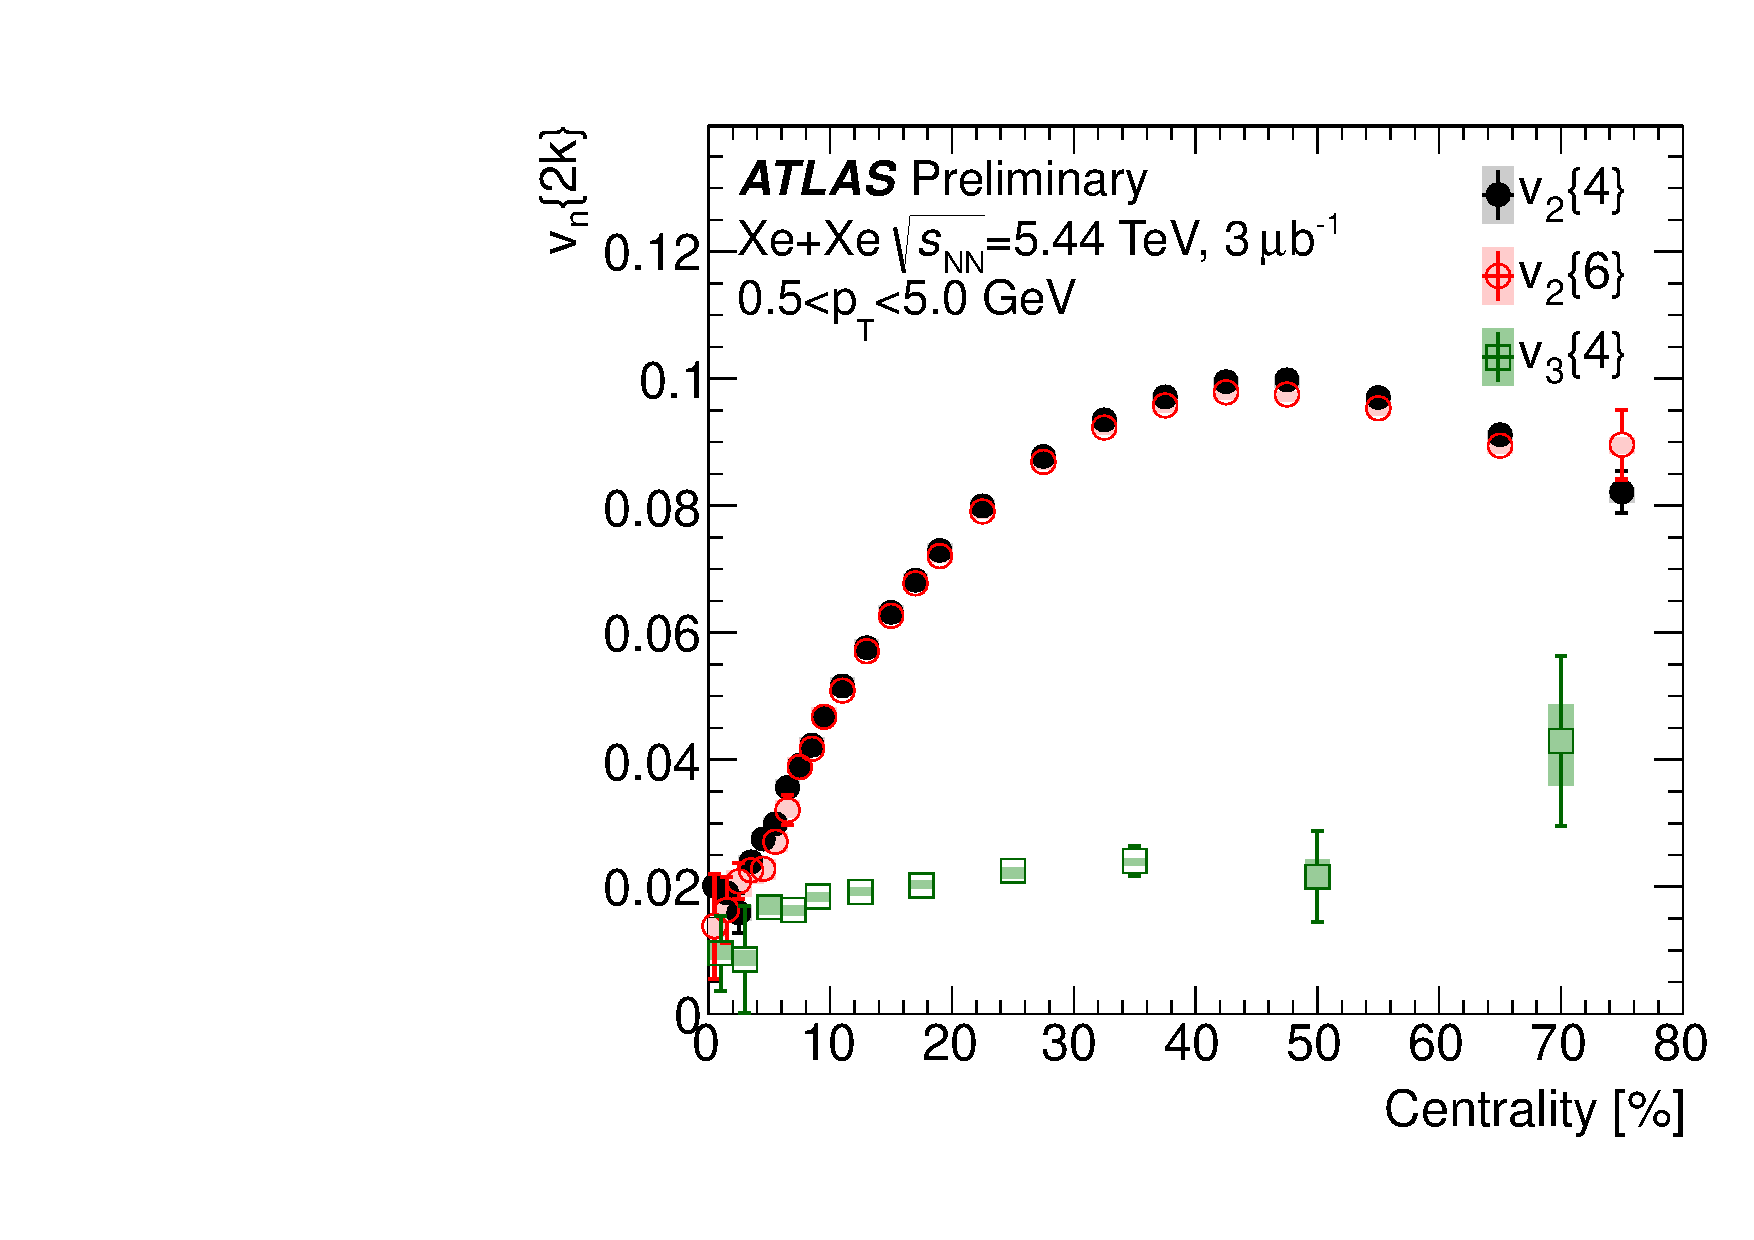
\includegraphics[width=.32\linewidth]{figs/chapter_centfluc/ATLAS_Xe_cn.pdf}
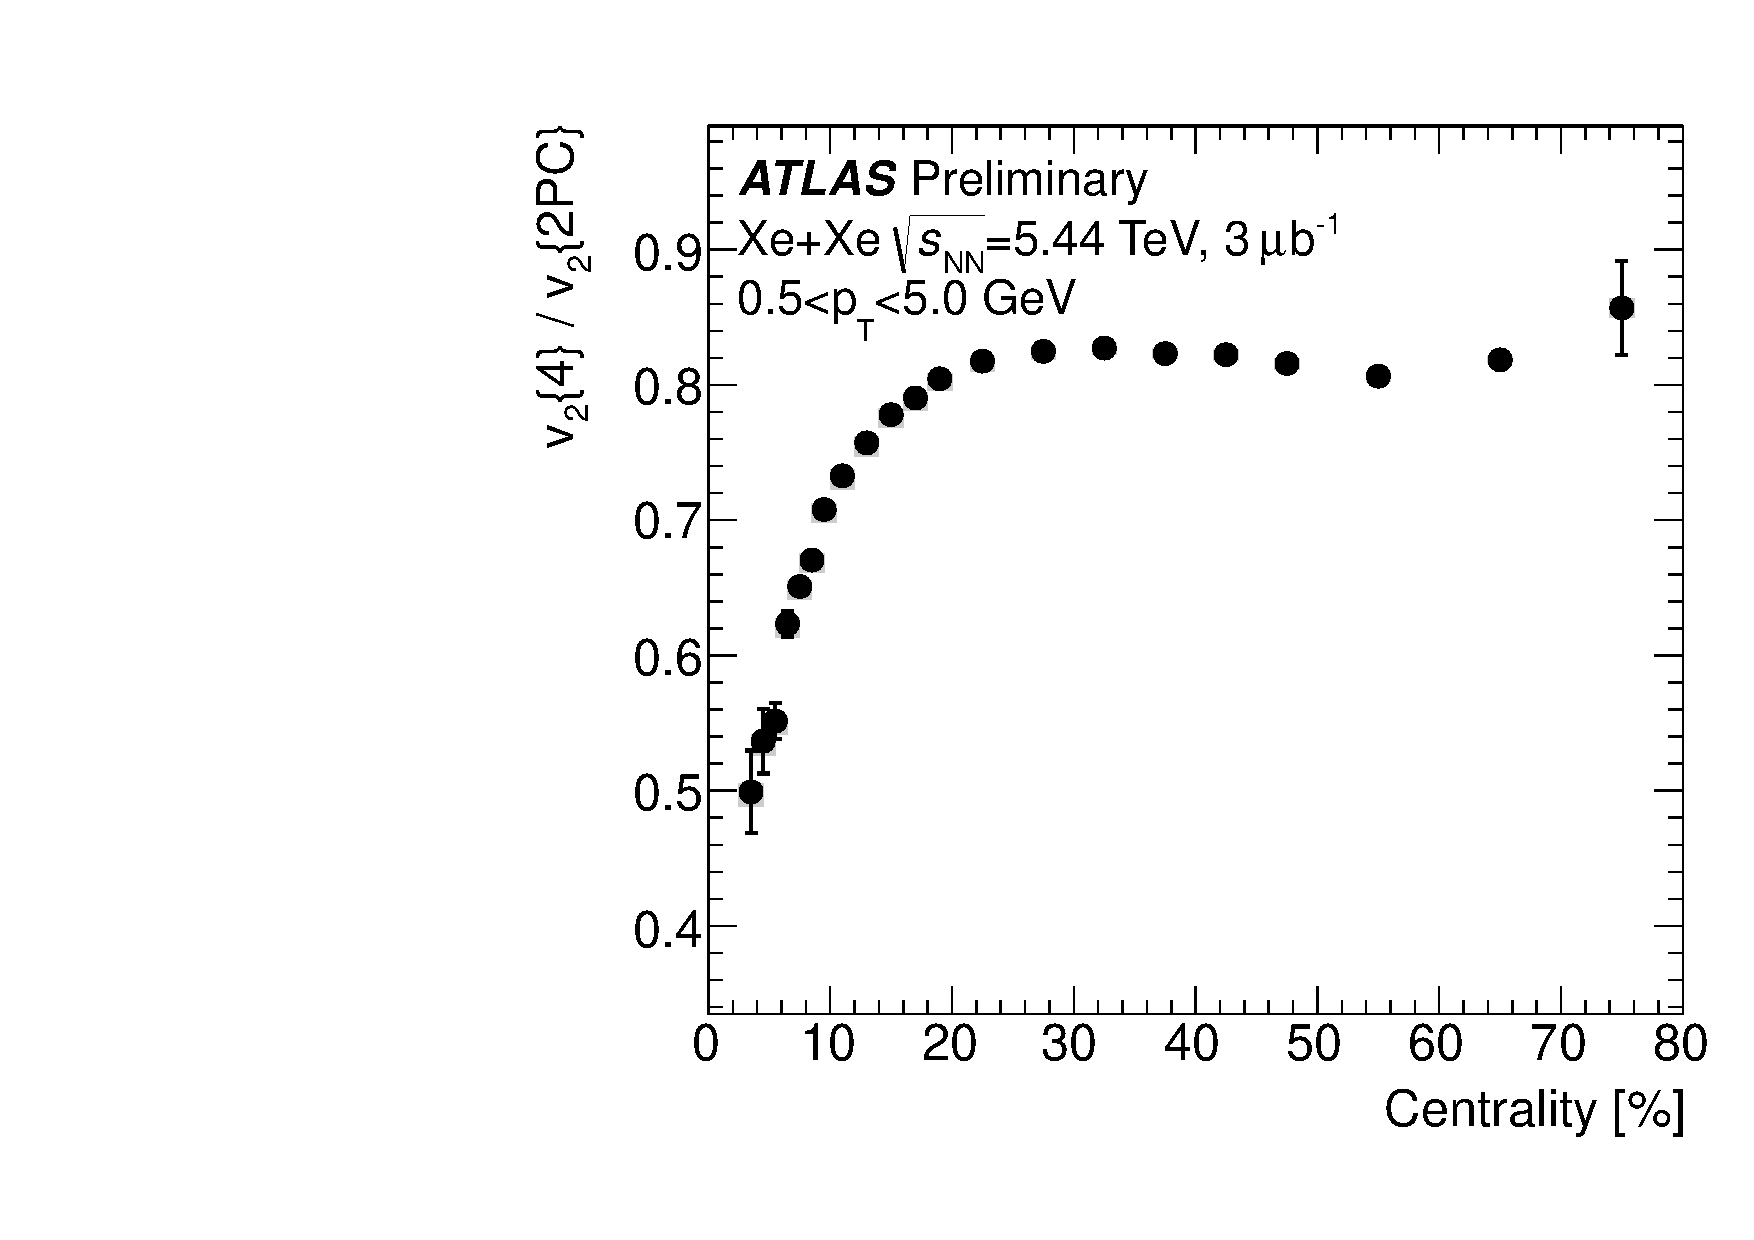
\includegraphics[width=.32\linewidth]{figs/chapter_centfluc/ATLAS_Xe_v42_ratio.pdf}
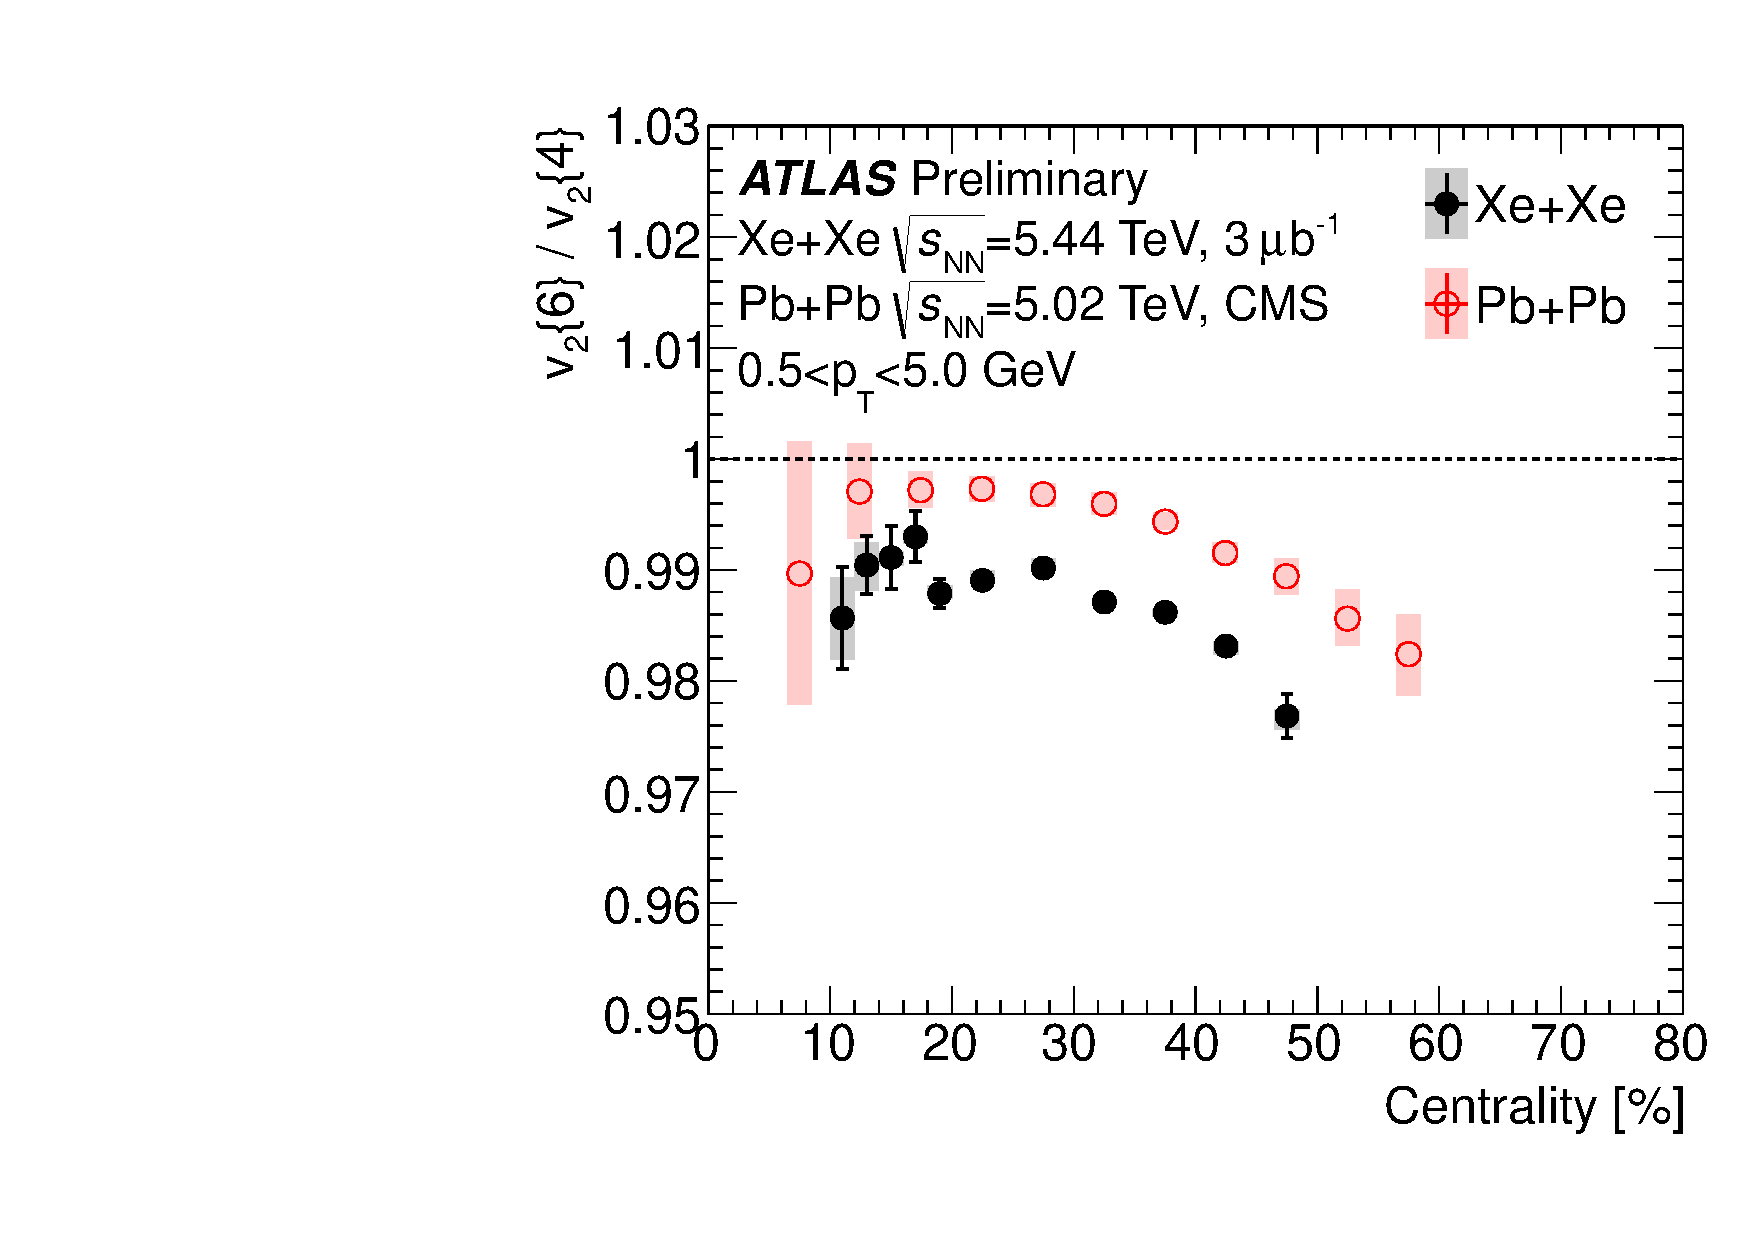
\includegraphics[width=.32\linewidth]{figs/chapter_centfluc/ATLAS_Xe_v64_ratio.pdf}
\caption{Left panel: 4- and 6-particle flow cumulants $v_n\{2k\}$ as a function of centrality, with particles in $0.5<\pT<5.0$ GeV. Middle panel: cumulant ratio $v_2\{4\} / v_2\{\text{2PC}\}$ as a function of centrality, where $v_2\{\text{2PC}\}$ is measured using the 2PC method. Right panel: cumulant ratio $v_2\{6\} / v_2\{4\}$ from Xe+Xe compared with Pb+Pb results, obtained using an unfolding technique from the CMS collaboration~\cite{Sirunyan:2017fts}. The shaded box represent the quadrature sum of statistical and systematic uncertainties.}
\label{fig:centfluc_ATLAS_Xe_cn}
\end{figure}

Figure~\ref{fig:centfluc_ATLAS_Xe_Pb_vn} shows the comparisons of multi-particle cumulants $c_n\{4\}$ in Xe+Xe with corresponding Pb+Pb measurements at $\sqrt{s_\text{NN}}=5.02$ TeV, as a function centrality or of the mean number of participants $\lr{N_\text{part}}$. In both cases, $c_2\{4\}$ in Xe+Xe is smaller than that in Pb+Pb except for peripheral collisions, which suggests that $v_2\{4\}$ is mainly driven by the average geometry of the initial stage. For $c_3\{4\}$ the Xe+Xe and Pb+Pb values scale better with $\lr{N_\text{part}}$ than centrality, which implies that $c_3\{4\}$ is mostly driven by the fluctuation of initial eccentricity. For $c_4\{4\}$, in mid-central and peripheral, the magnitudes are also comparable between Xe+Xe and Pb+Pb when shows as a function of $\lr{N_\text{part}}$. Furthermore, $c_4\{4\}$ is found to be larger than zero from mid-central to peripheral collisions, consistent with a non-linear mode-mixing between $v_2$ and $v_4$~\cite{Giacalone:2016mdr}.

\begin{figure}[H]
\centering
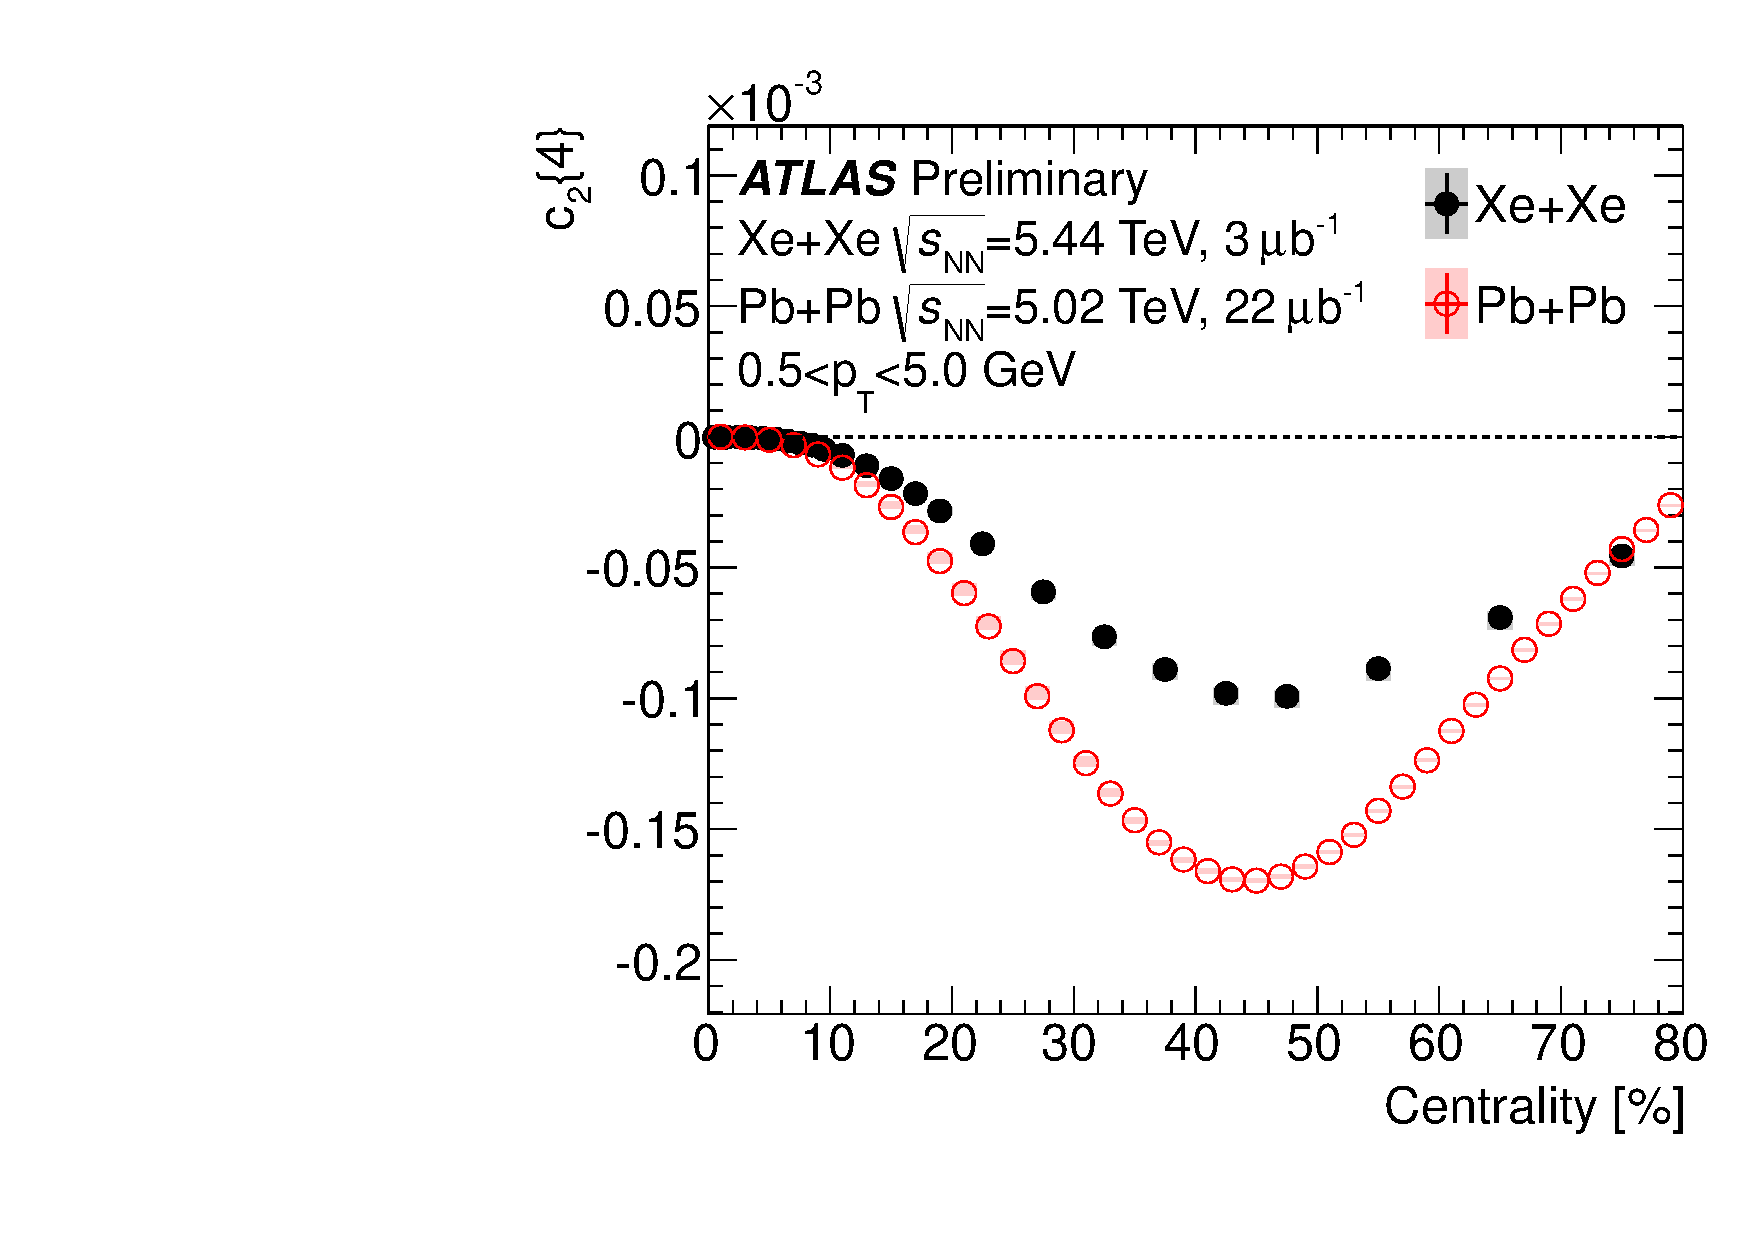
\includegraphics[width=.32\linewidth]{figs/chapter_centfluc/ATLAS_Xe_Pb_v2_cent1.pdf}
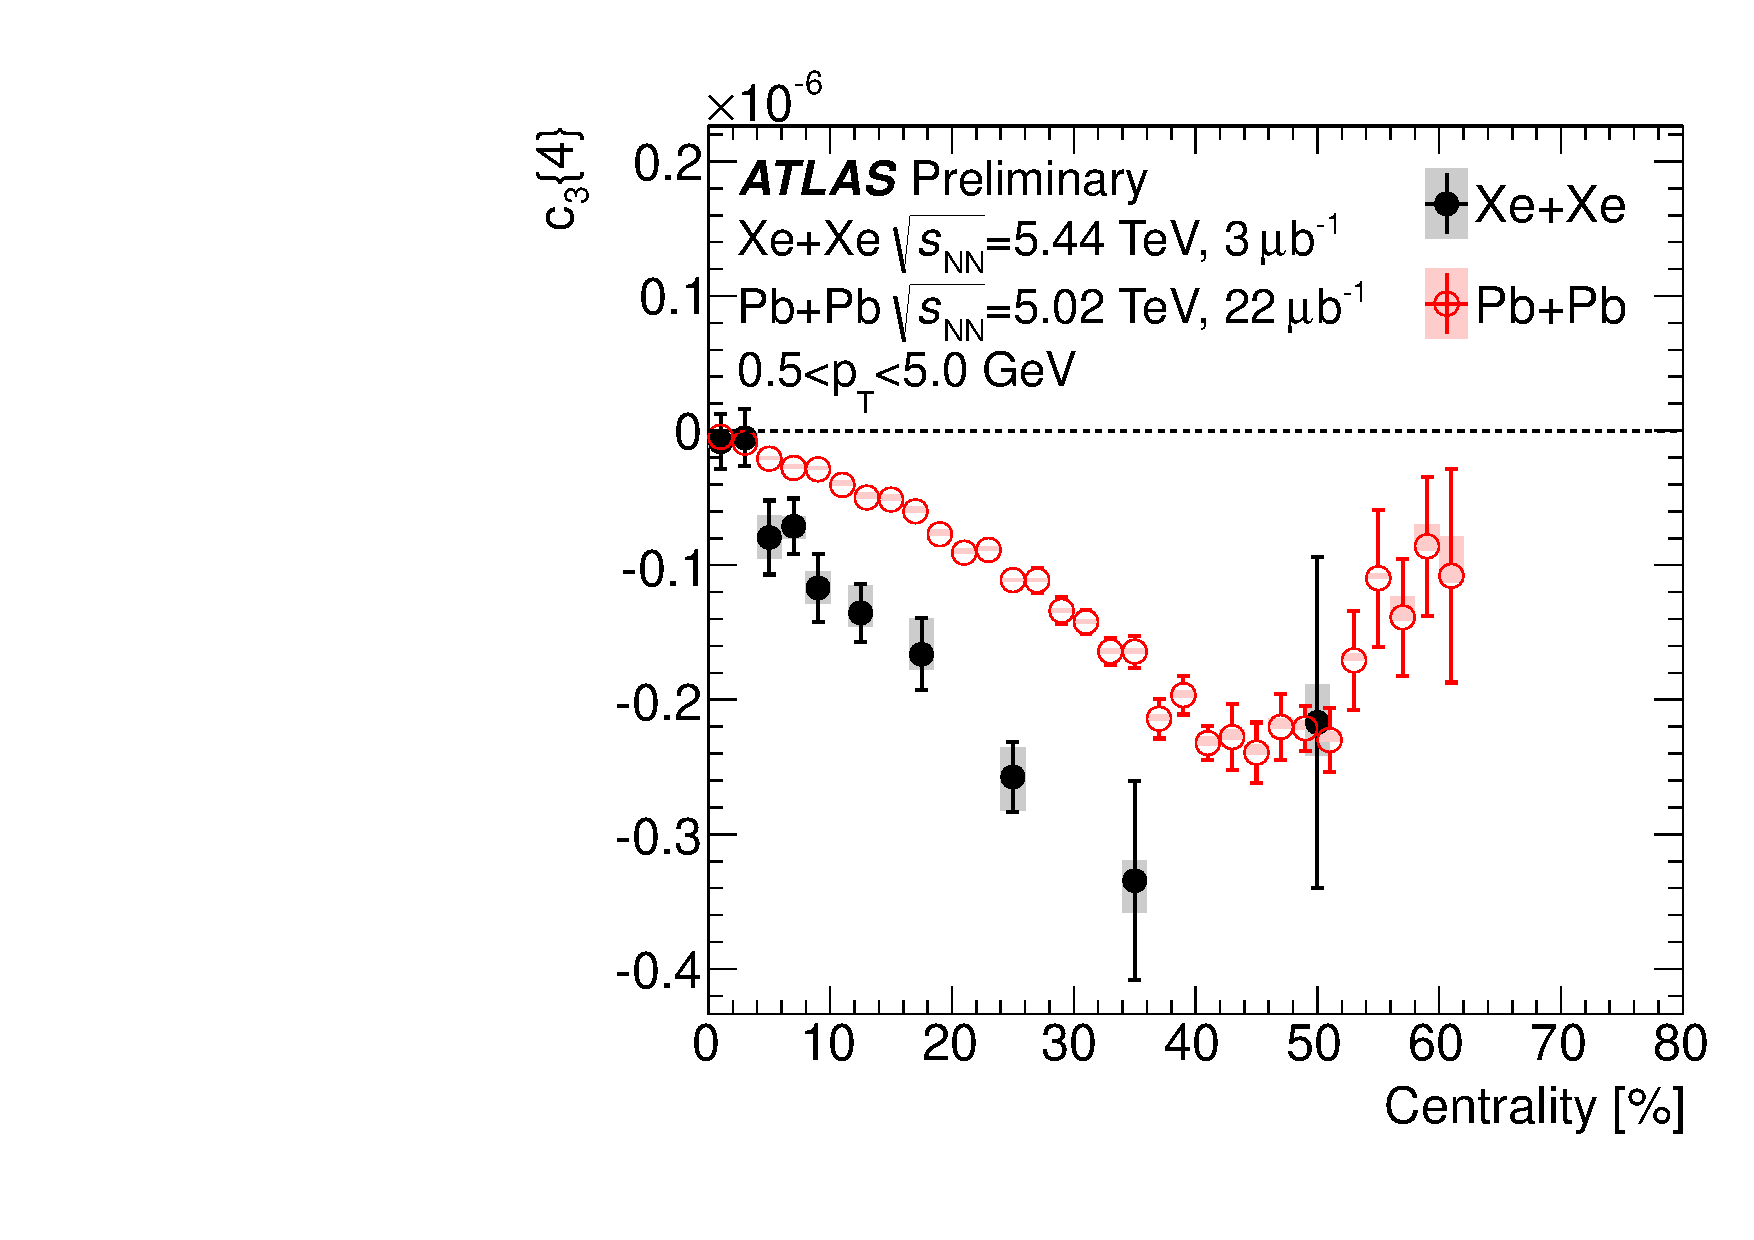
\includegraphics[width=.32\linewidth]{figs/chapter_centfluc/ATLAS_Xe_Pb_v3_cent1.pdf}
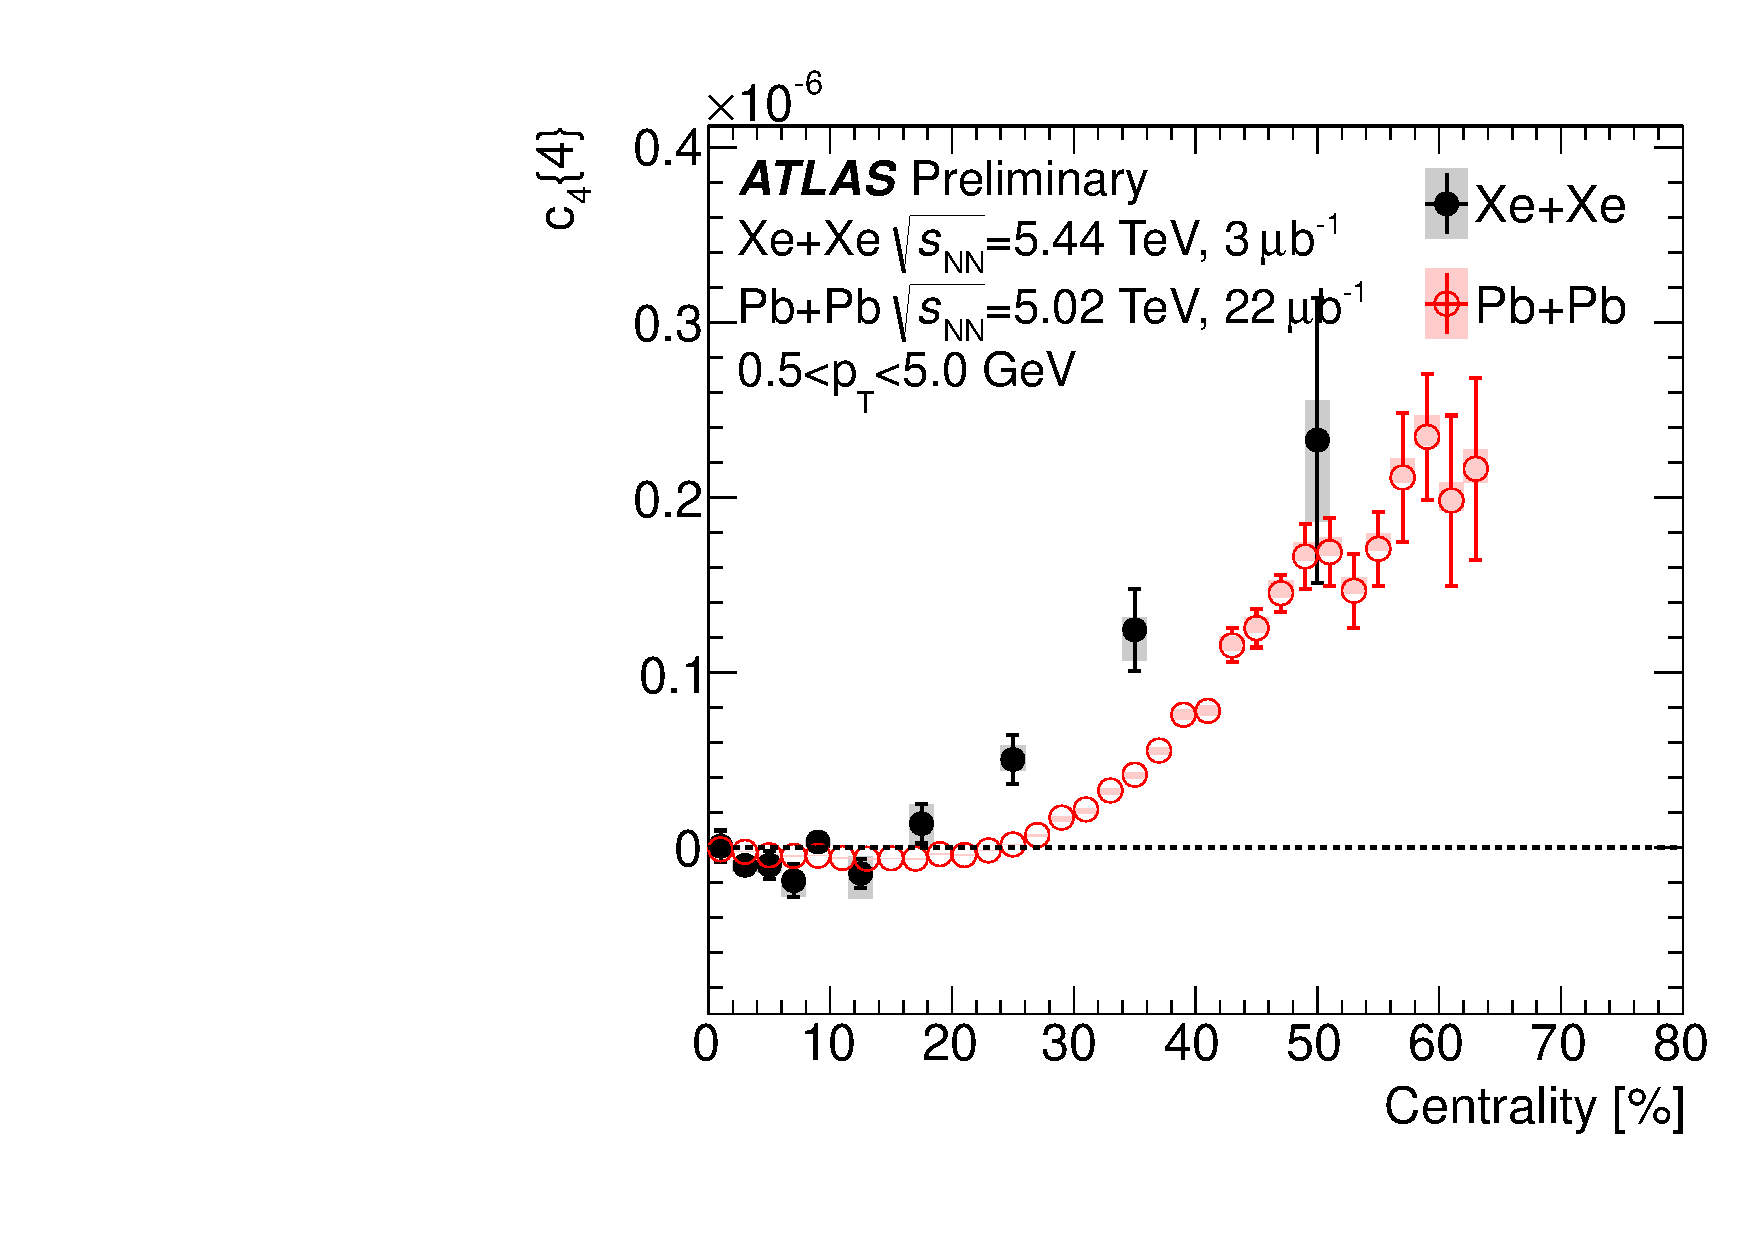
\includegraphics[width=.32\linewidth]{figs/chapter_centfluc/ATLAS_Xe_Pb_v4_cent1.pdf}
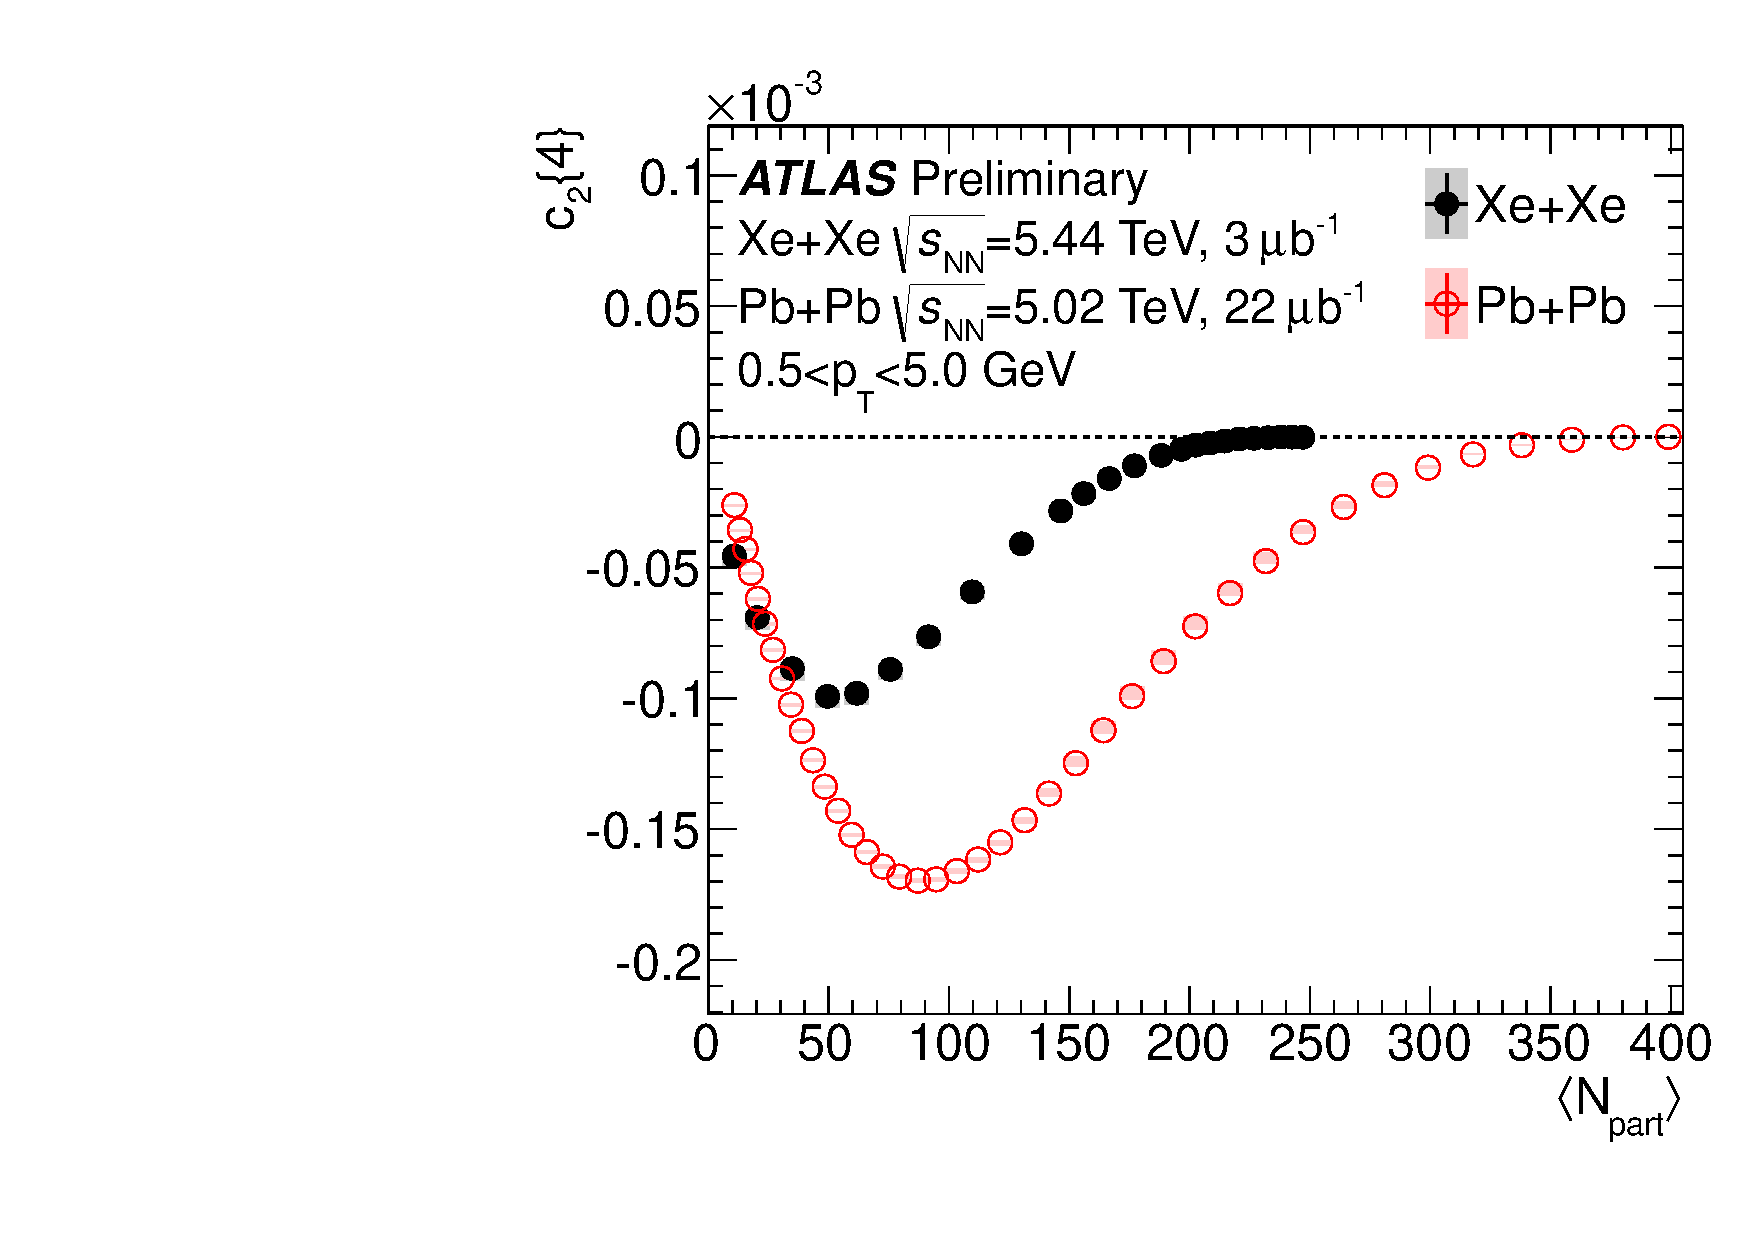
\includegraphics[width=.32\linewidth]{figs/chapter_centfluc/ATLAS_Xe_Pb_v2_cent2.pdf}
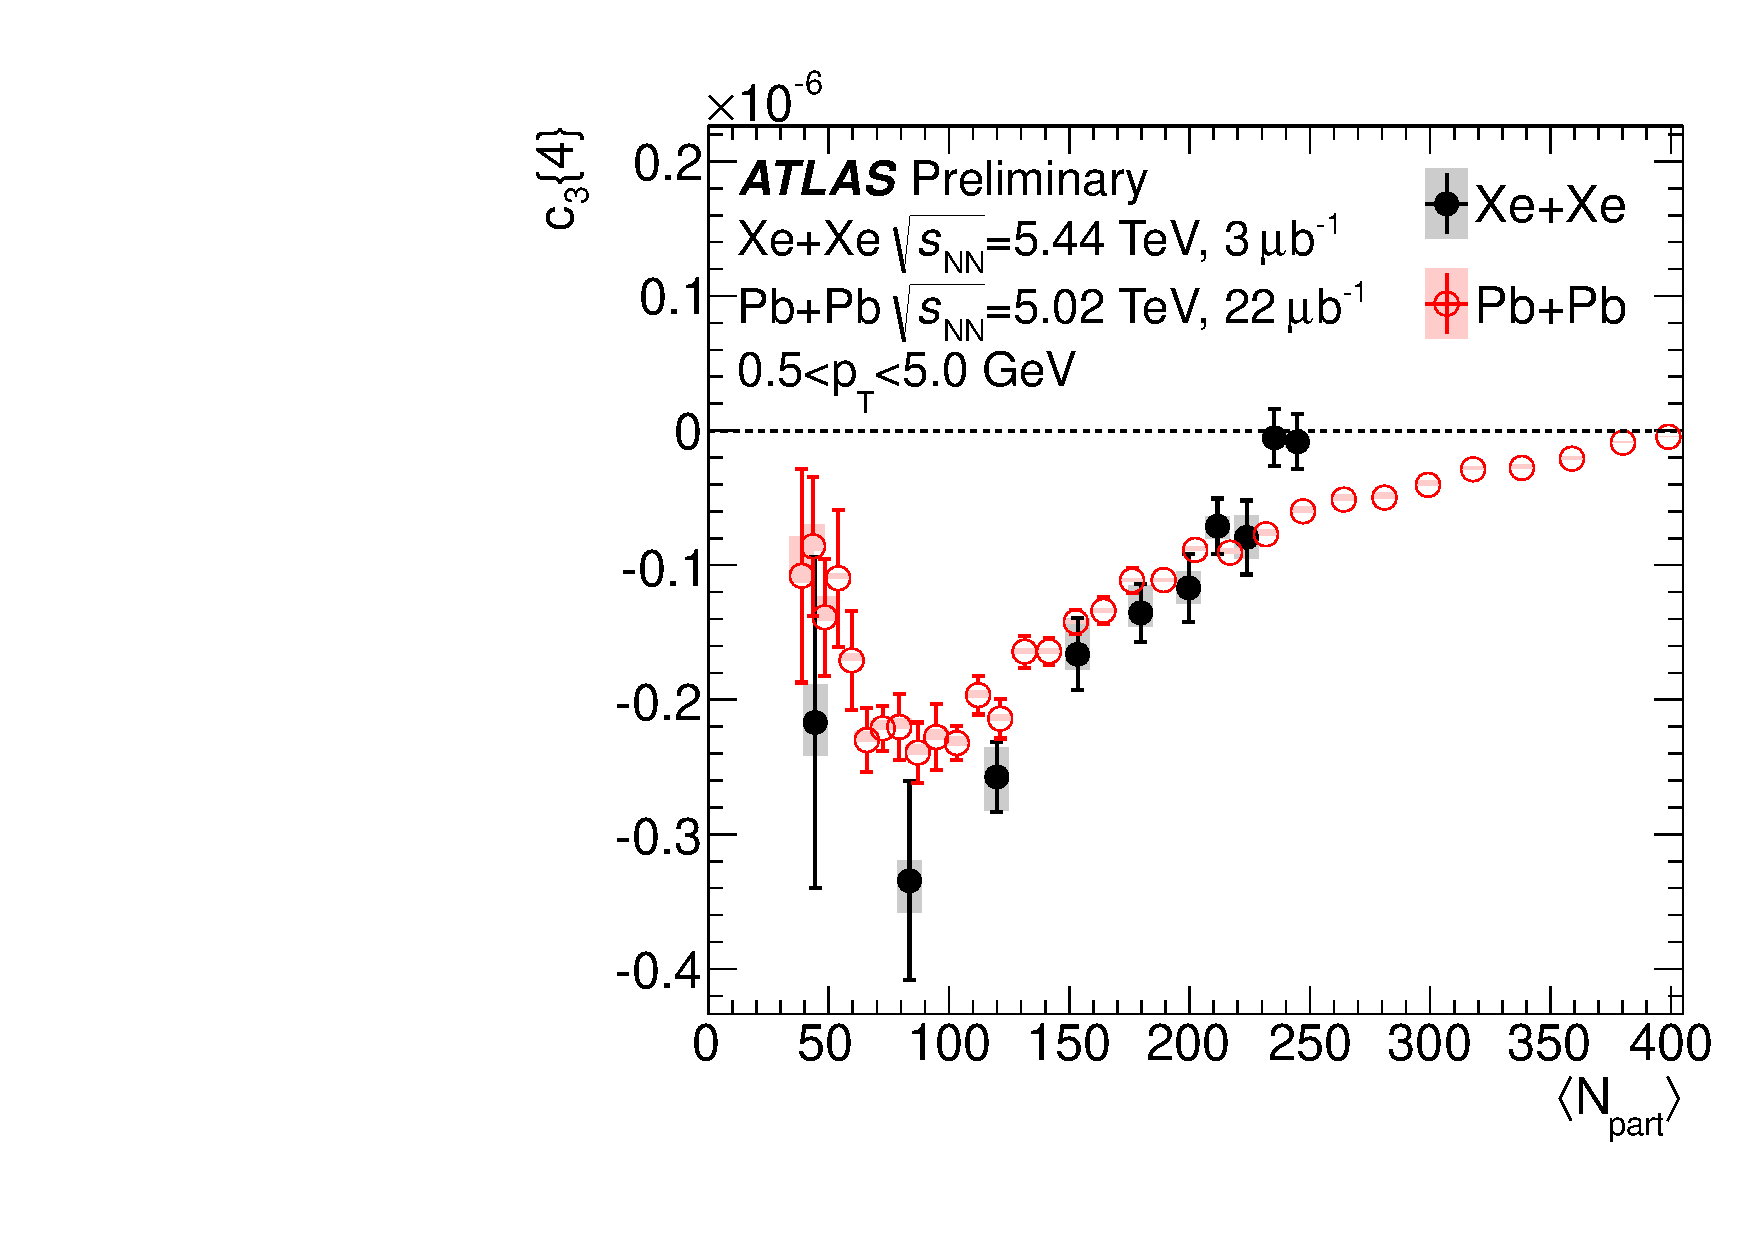
\includegraphics[width=.32\linewidth]{figs/chapter_centfluc/ATLAS_Xe_Pb_v3_cent2.pdf}
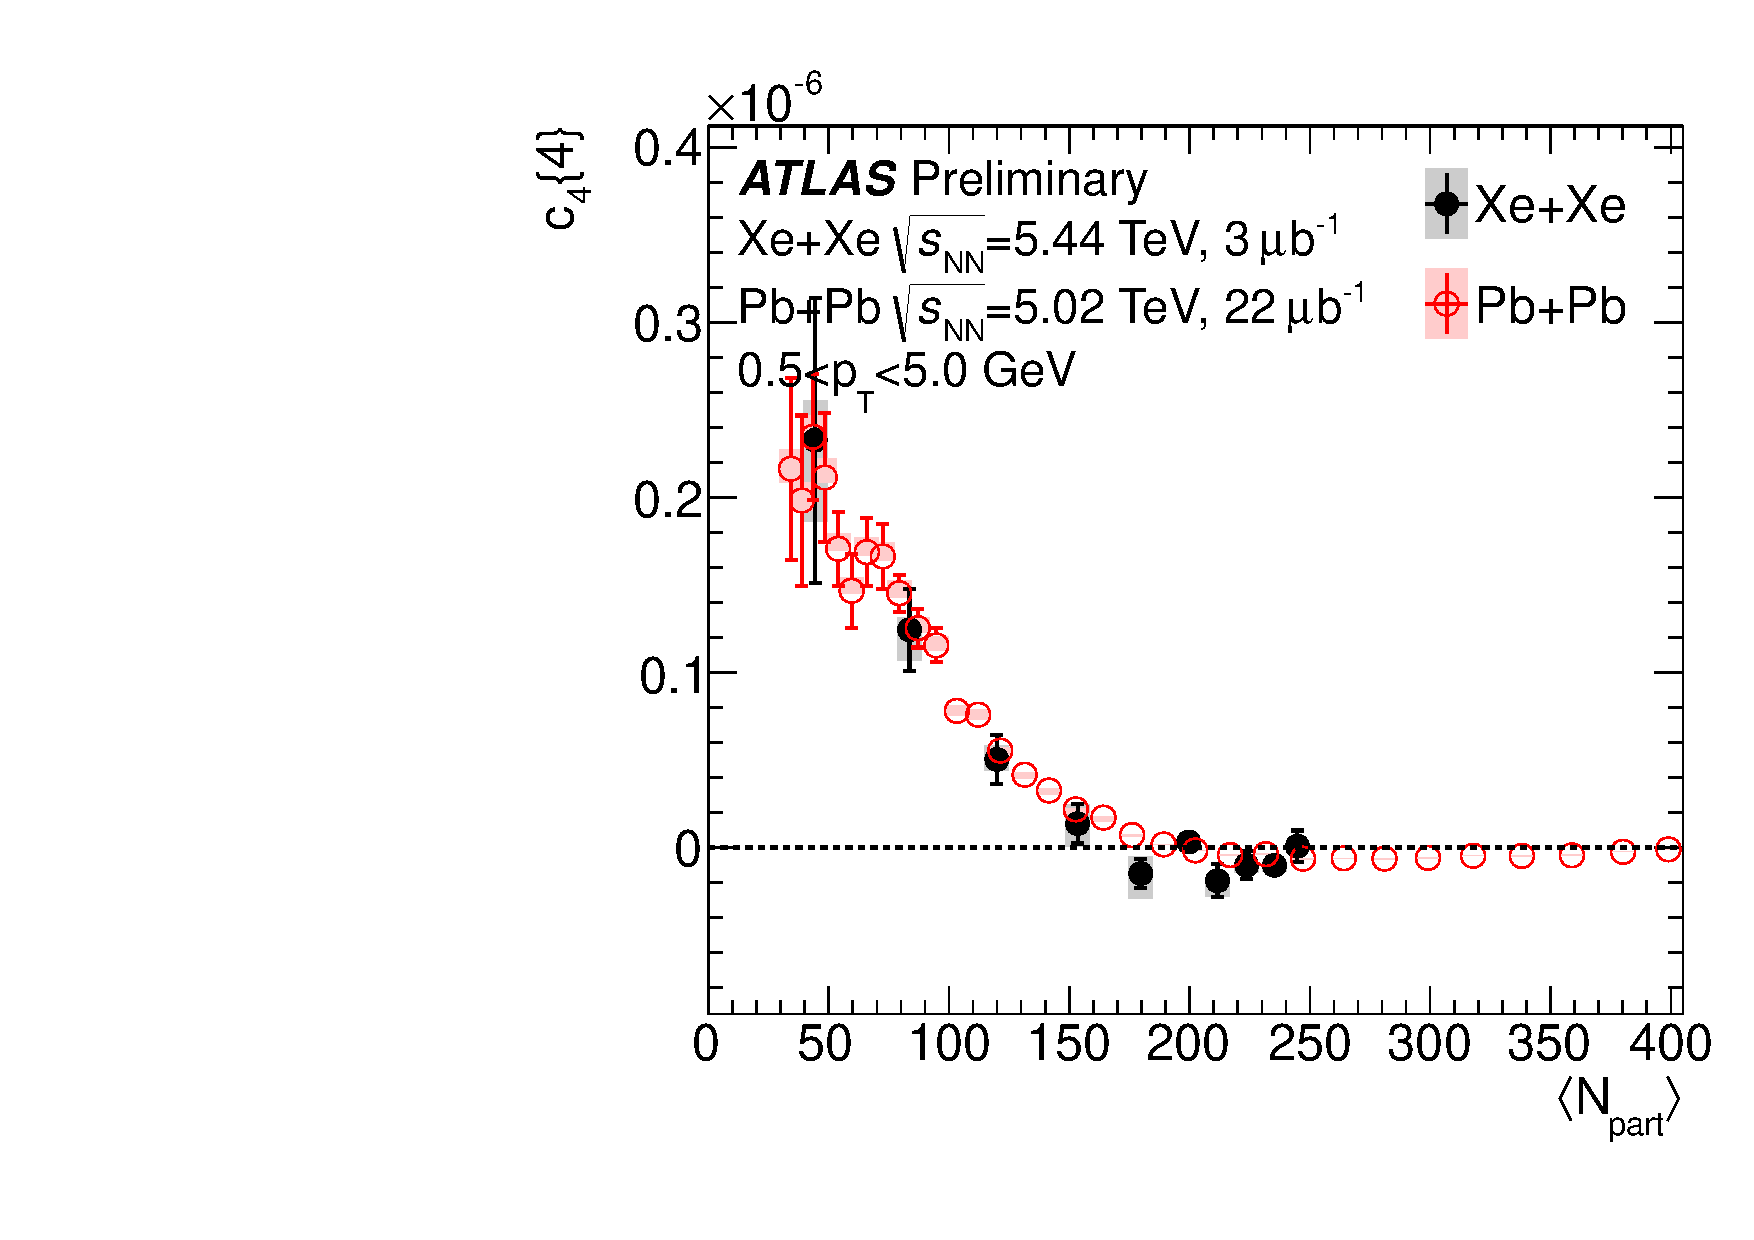
\includegraphics[width=.32\linewidth]{figs/chapter_centfluc/ATLAS_Xe_Pb_v4_cent2.pdf}
\caption{Comparisons of centrality (top) and $\lr{N_\text{part}}$ (bottom) dependence of the $c_n\{4\}$ measured in Pb+Pb collisions~\cite{ATLAS-CONF-2017-066} at $\sqrt{s_\text{NN}}=5.02$ TeV to present Xe+Xe measurements, for particles in $0.5<\pT<5.0$ GeV. Three columns are $c_2\{4\}$, $c_3\{4\}$ and $c_4\{4\}$ respectively.}
\label{fig:centfluc_ATLAS_Xe_Pb_vn}
\end{figure}

Figure~\ref{fig:centfluc_ATLAS_Xe_vn_diff} shows the $\pT$ dependence of the 4-particle differential flow cumulant $v_n\{4\}$. Each panel is a different centrality interval, and the results cover the $0-60\%$ centrality range. For all centralities, both $v_2\{4\}$ and $v_3\{4\}$ show similar $\pT$ dependence: they increase at low $\pT$ and reach a maximum between $2-4$ GeV and then decrease. In the high$-\pT$ region the decrease seems to stop. Overall the magnitude of $v_3$ is smaller than the magnitude of $v_2$ for all $\pT$ ranges.

\begin{figure}[H]
\centering
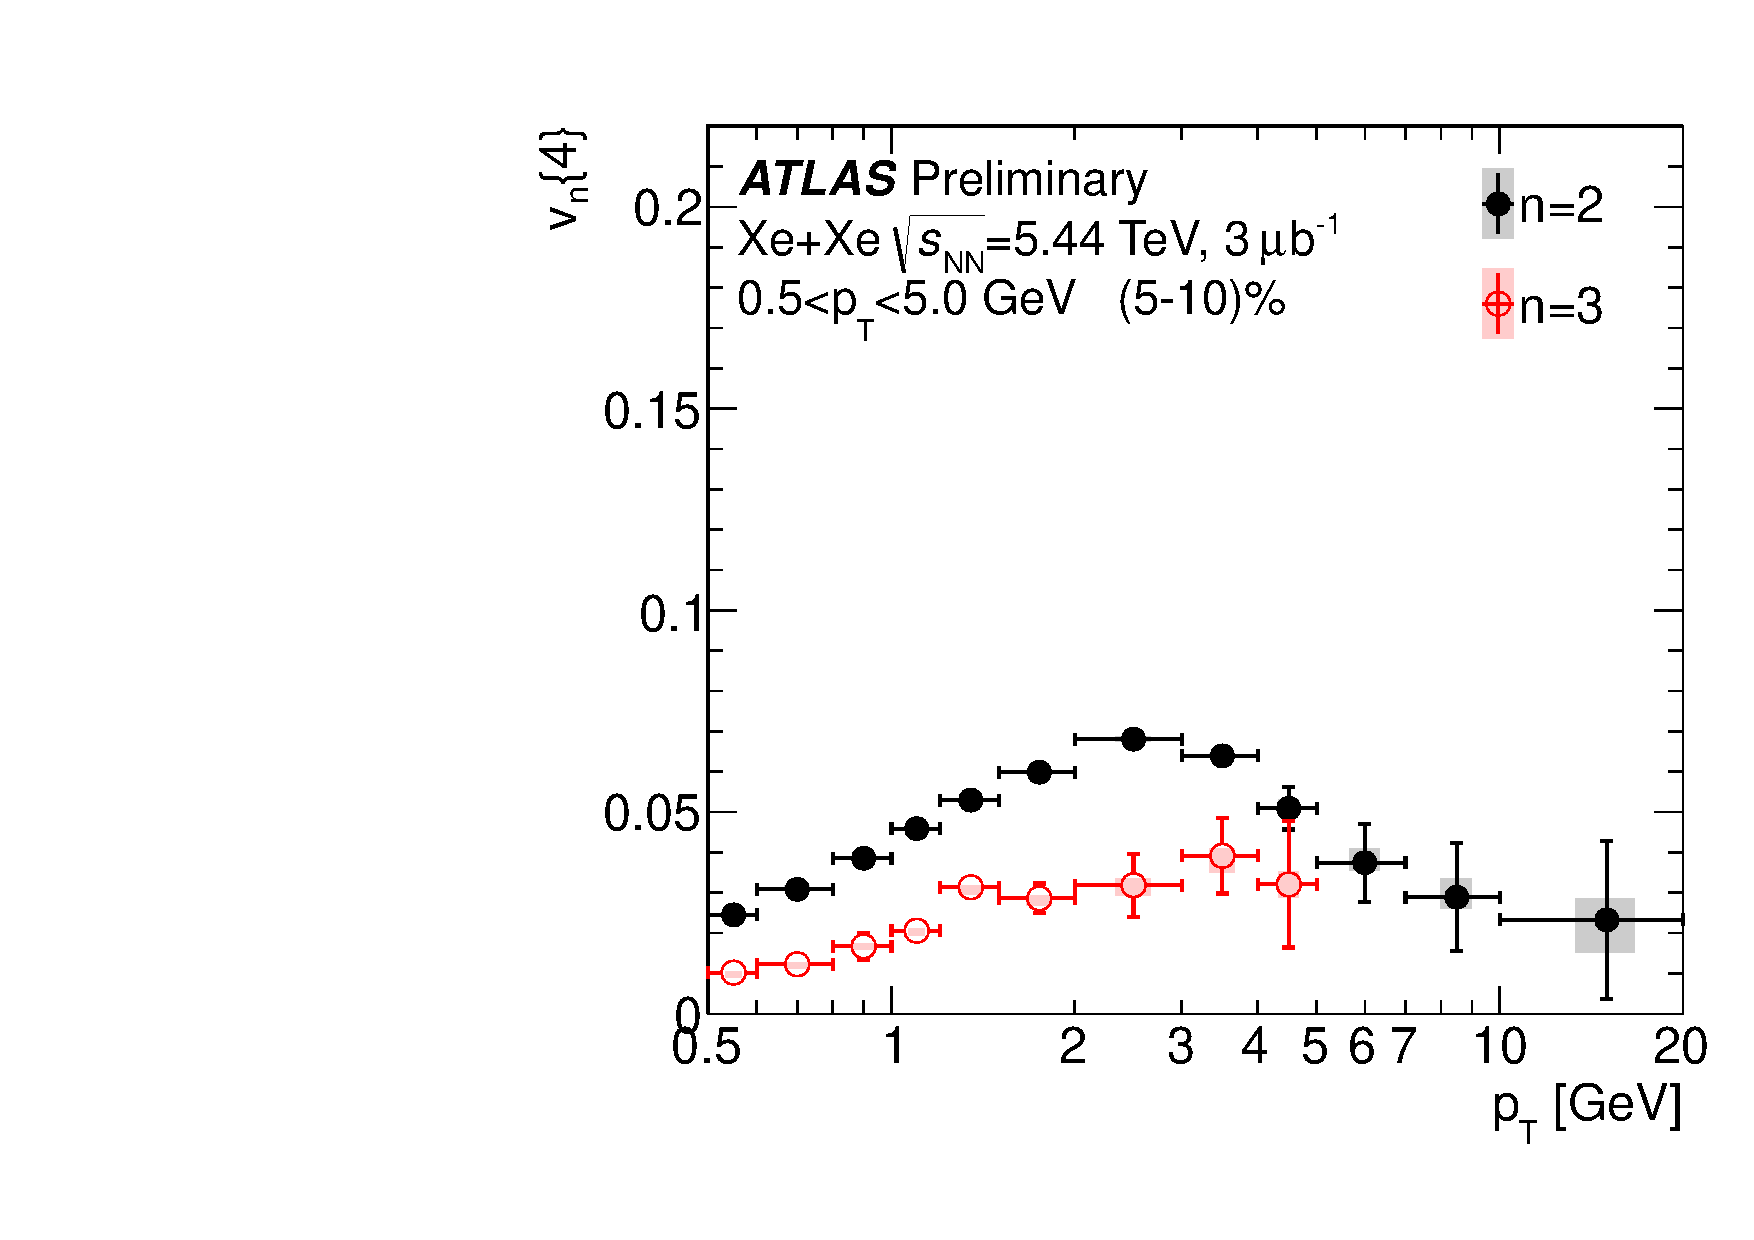
\includegraphics[width=.32\linewidth]{figs/chapter_centfluc/ATLAS_Xe_vn_diff_cent1.pdf}
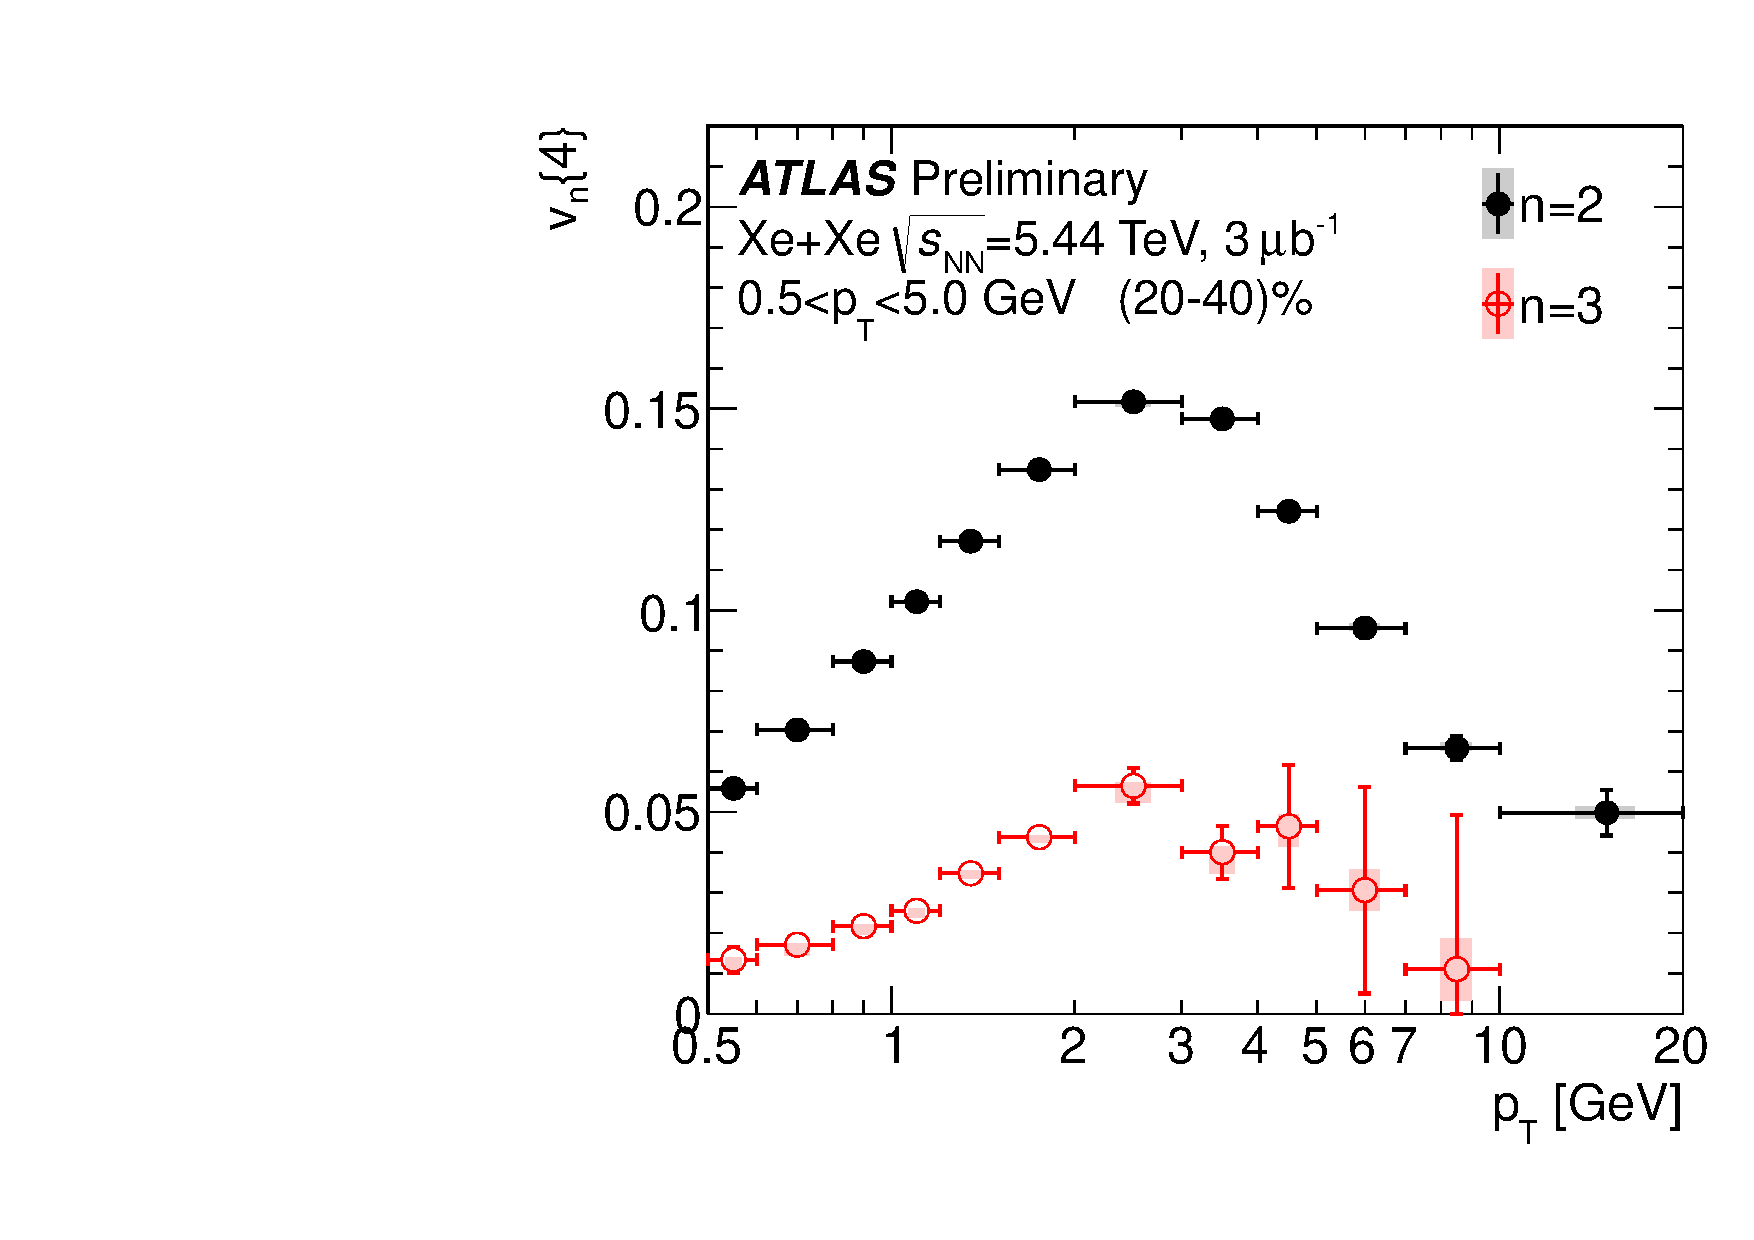
\includegraphics[width=.32\linewidth]{figs/chapter_centfluc/ATLAS_Xe_vn_diff_cent2.pdf}
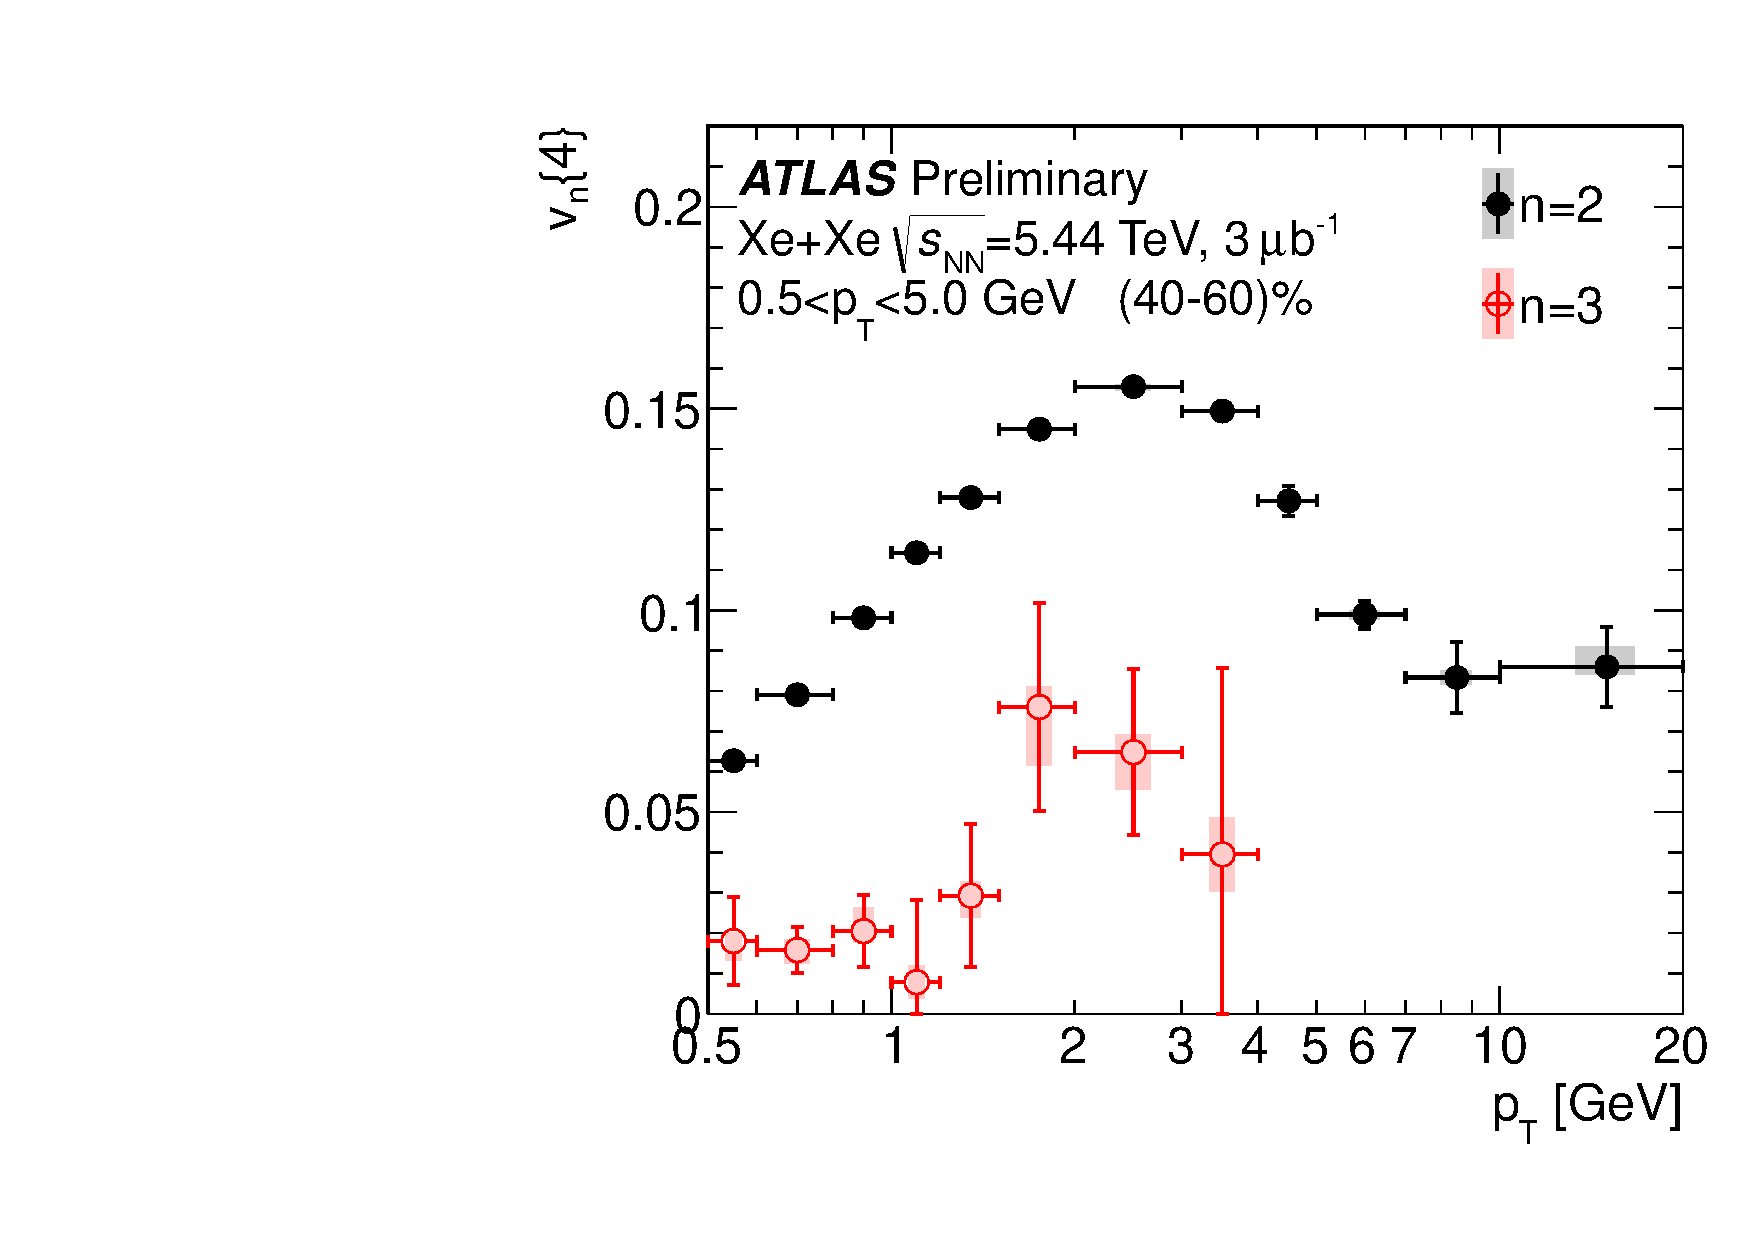
\includegraphics[width=.32\linewidth]{figs/chapter_centfluc/ATLAS_Xe_vn_diff_cent3.pdf}
\caption{The $\pT$ dependence of 4-particle differential flow cumulant $v_n\{4\}$. Each panel is a different centrality interval.}
\label{fig:centfluc_ATLAS_Xe_vn_diff}
\end{figure}

The left panel of Figure~\ref{fig:centfluc_ATLAS_Xe_sc} shows the centrality dependence of symmetric and asymmetric cumulants, using particles with $0.5<\pT<5.0$ GeV. A negative $sc_{2,3}\{4\}$ is observed over the entire centrality range, indicating that $v_2$ and $v_3$ are anti-correlated. The positive $sc_{2,4}\{4\}$ reflects the correlation between non-linear hydrodynamic response of $v_2$ and the linear component of $v_4$. The asymmetric cumulant $ac_{2}\{3\}$ shows a similar centrality dependence as $sc_{2,4}\{4\}$, but with a larger magnitude. The right panel shows the normalized symmetric and asymmetric cumulants. The magnitudes of all three correlators keep increasing towards peripheral, suggesting that the centrality dependence of $sc_{n,m}\{4\}$ and $ac_2\{3\}$ originates mainly from the $\lr{v_n^2}$. The correlations are very weak in central collisions, but increase rapidly towards peripheral collisions.

\begin{figure}[H]
\centering
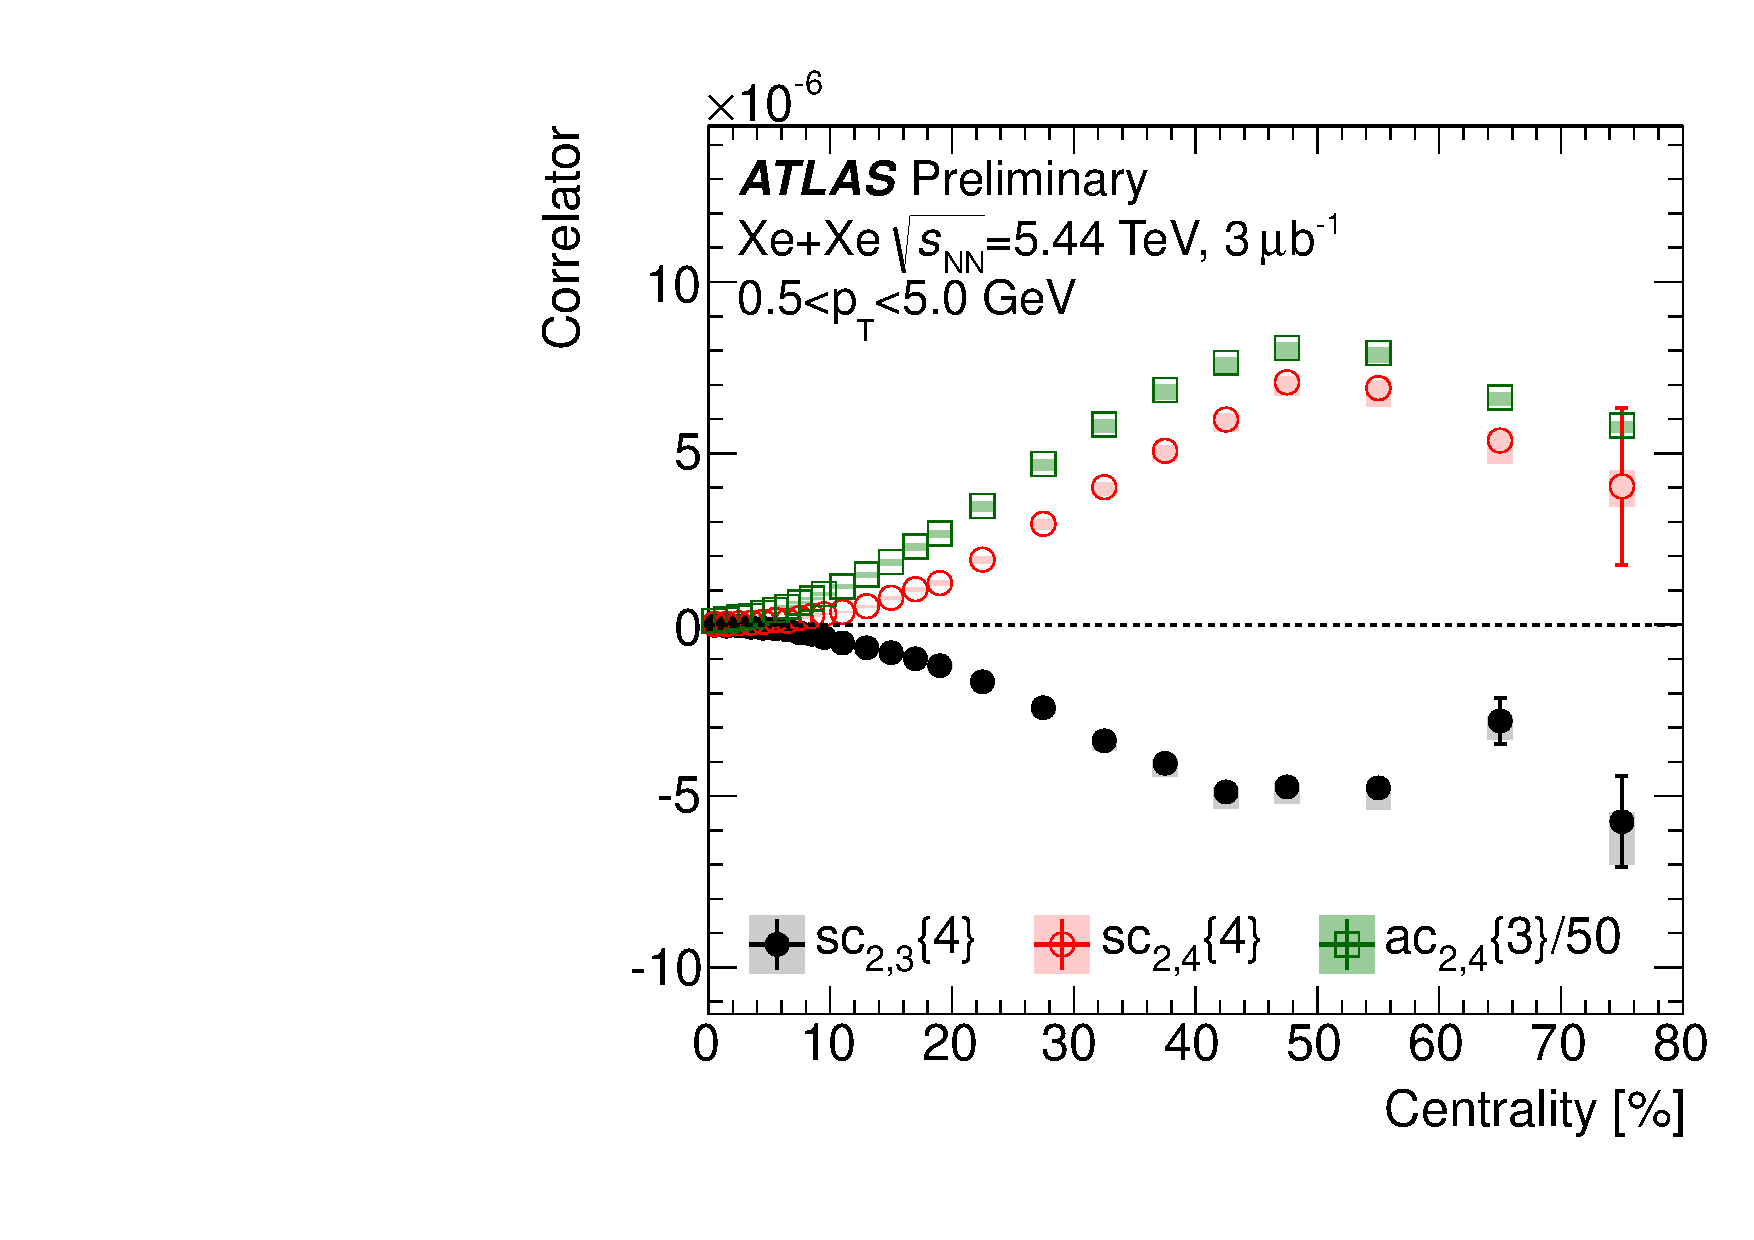
\includegraphics[width=.475\linewidth]{figs/chapter_centfluc/ATLAS_Xe_sc.pdf}
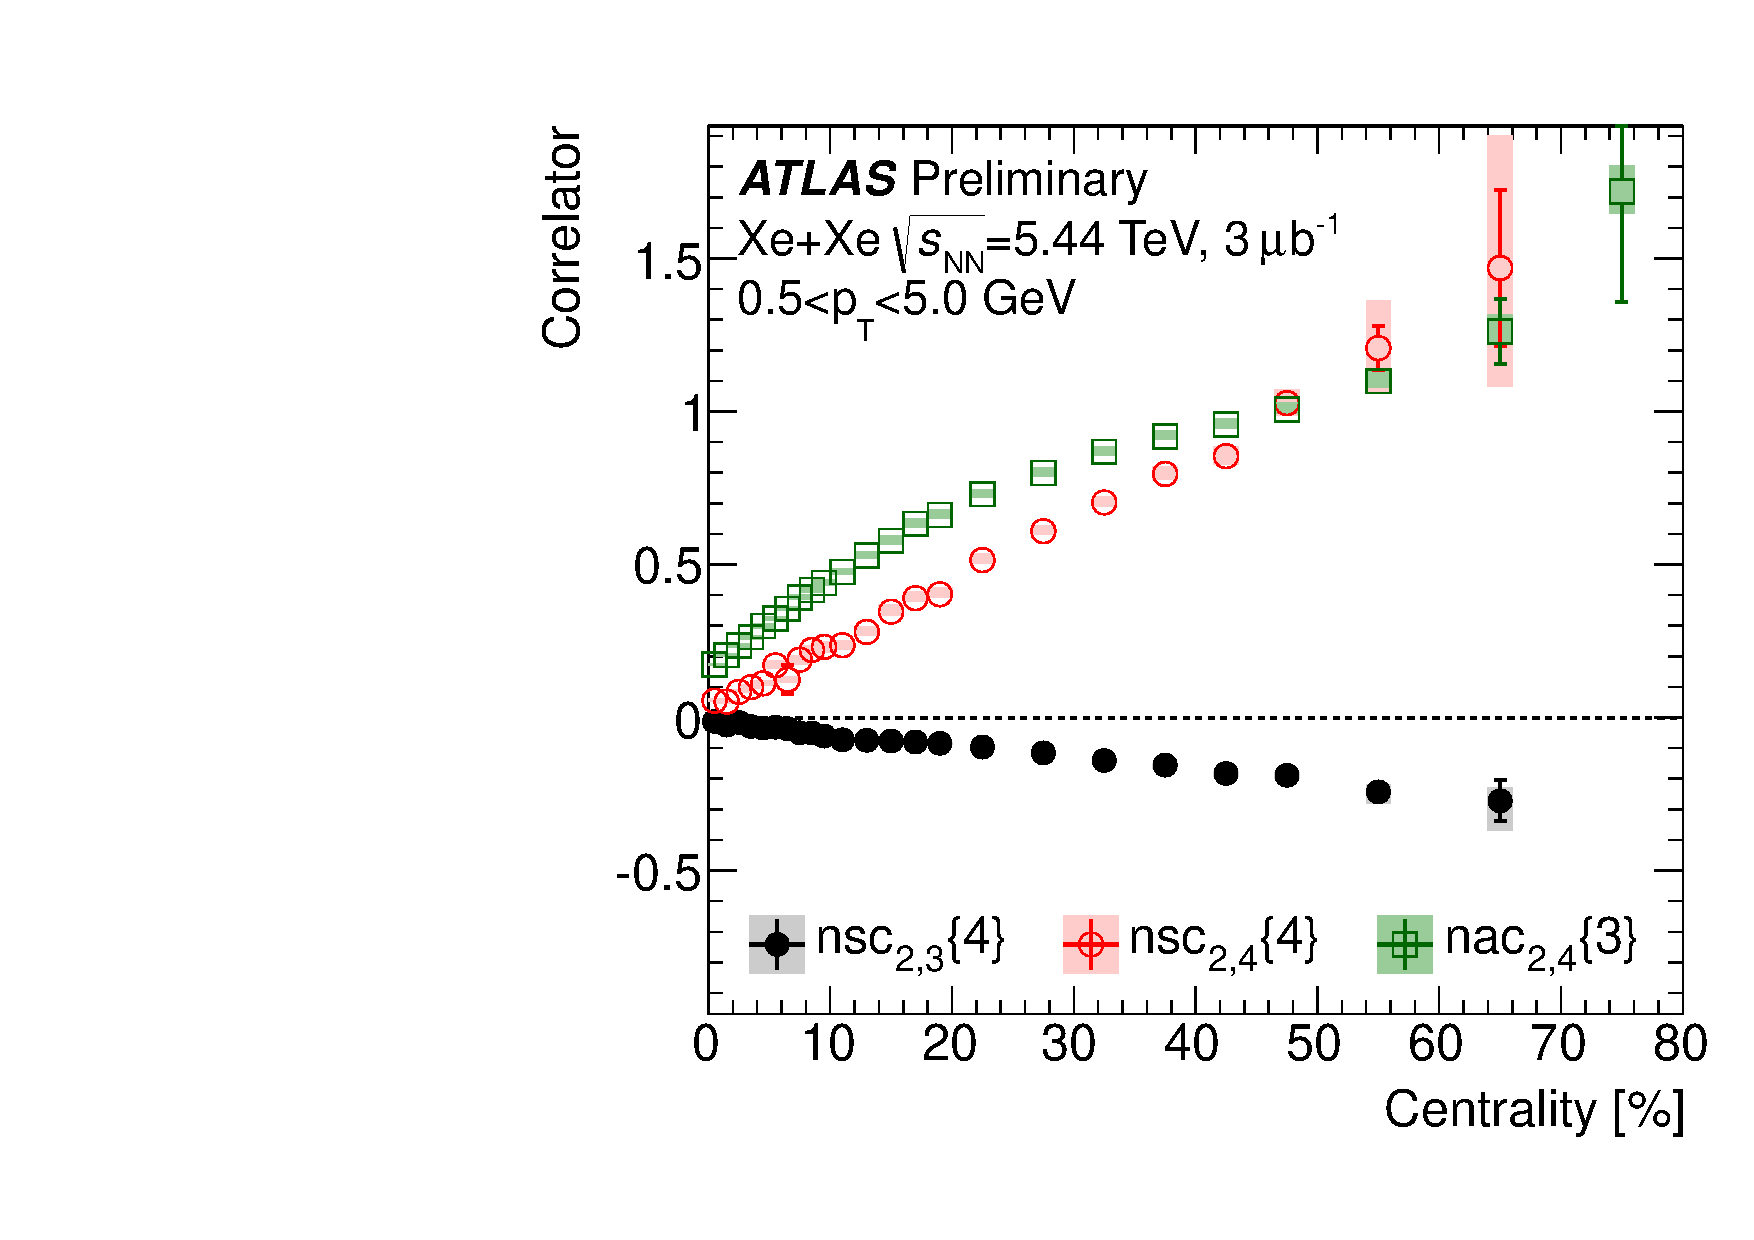
\includegraphics[width=.475\linewidth]{figs/chapter_centfluc/ATLAS_Xe_nsc.pdf}
\caption{Symmetric and asymmetric cumulants (left), normalized symmetric and asymmetric cumulants (right). Cumulants are evaluated as a function of centrality, with particles in $0.5<\pT<5.0$ GeV.}
\label{fig:centfluc_ATLAS_Xe_sc}
\end{figure}



\subsubsection{More realistic models}

Obviously, the independent source model based on Glauber and NBD has certain limitations on its predictive power. It does not model the interaction between different sources, which clearly is important in the final state. These interactions may modify the particle correlations in each source or create new sources of fluctuations.

Furthermore, our present study assumes that the sources are boost invariant in the longitudinal direction. In reality, the number of sources $N_\text{s}$ as well as their distributions in the transverse plane may fluctuation in rapidity:
\begin{itemize}
\item In models based on string picture~\cite{Bozek:2015bna, Pang:2015zrq, Shen:2017bsr}, the number of strings, their lengths, and their endpoints in rapidity fluctuate.
\item The sub-nucleonic degrees of freedom are expected to evolve with rapidity~\cite{Schenke:2016ksl}: In the forward rapidity, the projectile nucleons are dominated by a few large-$x$ partons, while the target nucleons are expected to contribute mainly low-$x$ soft gluons.
\item The number of forward-going and backward-going participating nucleons, $N_\text{part}^\text{F}$ and $N_\text{part}^\text{B}$, are not the same in a given event~\cite{Jia:2015jga, Jia:2014ysa}.
\end{itemize}
For these reasons, the $N_\text{s}$ in general should be a function of $\eta$ even in a single event, which tends to weaken the centrality correlation between different rapidities. This also means that a simple combination of particles from two very different rapidity regions may not improve the centrality resolution if the longitudinal fluctuations are large. This simple independent source model can be extended in this direction in the future.

We believe that the study of the inter-event longitudinal fluctuations as a way to infer the bulk characteristic of the entire A+A event will be an important direction of heavy-ion research. Subevent correlation or subevent cumulant method is a valuable tool to disentangle physics happening at different timescales. Initial studies on flow and multiplicity fluctuations have been performed at RHIC and the LHC but with rather limited $\eta$ range, comparing to their respective beam rapidities. At RHIC, the STAR experiment has embarked on a very significant forward upgraded program, which extends the rapidity coverage for particle identification from $|\eta|<0.9$ to $|\eta|<1.5$~\cite{LinkSTAR:2015tdr}, as well as instrumenting the forward region $2.5<\eta<4.0$ with tracking detector and calorimeter~\cite{LinkSTAR:2016fcs}. A forward upgrade has also been planned for the PHENIX experiment~\cite{Adare:2015kwa}. Experiments at LHC also proposed forward upgrades~\cite{LinkLHC:2017whl}, mostly notably the upgrades from ATLAS and CMS to extend rapidity coverage of tracking from $|\eta|<2.5$ to $|\eta|<4$. Another interesting possibility is to directly measure $N_\text{part}$ in each event, therefore the $p(N_\text{part})$, by detecting all spectator fragments using a dedicated ``centrality detector''~\cite{Tarafdar:2014oua}, which should provide strong model-independent constraints on the centrality fluctuations. (This is an extension to the commonly used zero-degree calorimeter at RHIC and LHC, which detects only a small fraction of all spectators.) These upgrades will allow us to work toward a complete picture of the bulk characteristic of the entire event in the coming years.





